% !TeX program = pdflatex
% OVERLEAF FREE-PLAN / TIMEOUT-SAFE ENTRY POINT
% This project intentionally provides only one active root document: main.tex.
% It compiles in one pdfLaTeX pass using cached citations, labels, lists, and a
% static bibliography. Full local-build sources are stored as *.disabled under
% local_build_sources/ so Overleaf cannot select them accidentally.
\documentclass[
  12pt,
  a4paper,
  oneside,
  open=right,
  headings=big,
  bibliography=totoc,
  listof=totoc,
  numbers=enddot
]{scrreprt}

% Submission metadata. Confirm the exact submission day before the final upload.
\newcommand{\ThesisTitle}{Chatbot for Anatomy}
\newcommand{\ThesisShortTitle}{Chatbot for Anatomy}
\newcommand{\ThesisAuthor}{Adarsh Raj}
\newcommand{\MatriculationNumber}{287083}
\newcommand{\DegreeProgramme}{Artificial Intelligence and Machine Learning}
\newcommand{\UniversityName}{Hochschule Furtwangen University}
\newcommand{\FacultyName}{Faculty I: Computer Science \& Applications}
\newcommand{\FirstSupervisor}{Prof.\ Dr.\ Holger Ziekow}
\newcommand{\SecondSupervisor}{Prof.\ Dr.\ med.\ habil.\ Stephan Heermann}
\newcommand{\SubmissionPlace}{Furtwangen}
\newcommand{\SubmissionDate}{August 2026}
\newcommand{\RepositoryCommit}{d3a544d0b2202b1e068b648968a2ae17f871bfa8}

% -----------------------------------------------------------------------------
% FAST OVERLEAF PREAMBLE
% This version avoids TikZ/tcolorbox/Biber on every cloud compile.
% Diagrams are pre-rendered PDFs in figures/rendered/.
% Bibliography uses natbib + BibTeX for faster compilation.
% -----------------------------------------------------------------------------

% Encoding, language and typography
\usepackage[utf8]{inputenc}
\usepackage[T1]{fontenc}
\usepackage[main=english,ngerman]{babel}
\usepackage{lmodern}
\usepackage{csquotes}
\usepackage{setspace}
\usepackage{geometry}
\usepackage{scrlayer-scrpage}
\usepackage{etoolbox}

\geometry{
  left=3.2cm,
  right=2.6cm,
  top=2.6cm,
  bottom=2.8cm,
  headsep=0.8cm
}
\onehalfspacing
\KOMAoptions{parskip=half}
\setlength{\emergencystretch}{3em}

% Tables, figures, mathematics and code
\usepackage{graphicx}
\usepackage{booktabs}
\usepackage{longtable}
\usepackage{tabularx}
\usepackage{array}
\usepackage{amsmath,amssymb}
\usepackage{enumitem}
\usepackage{caption}
\usepackage{pdflscape}
\usepackage{listings}
\usepackage{xcolor}

% Fast author-year bibliography: BibTeX instead of Biber
\usepackage[round,authoryear]{natbib}
\renewcommand{\bibname}{References}
% Compatibility aliases so existing chapter files do not need rewriting.
\newcommand{\parencite}[1]{\citep{#1}}
\newcommand{\textcite}[1]{\citet{#1}}

% Links and references
\usepackage{xurl}
\usepackage[hidelinks]{hyperref}
\usepackage{bookmark}
\makeatletter
\renewcommand*{\@pnumwidth}{2.6em}
\makeatother
\usepackage[nameinlink,noabbrev,capitalise]{cleveref}
\hypersetup{
  pdftitle={\ThesisTitle},
  pdfauthor={\ThesisAuthor},
  pdfsubject={Master's thesis},
  pdfkeywords={retrieval-augmented generation, multimodal retrieval, anatomy education, Model Context Protocol, Blender, Z-Anatomy, Multimodal Anatomy Learning Assistant}
}

% Header and footer
\clearpairofpagestyles
\ihead{\headmark}
\ohead{\pagemark}
\automark[section]{chapter}
\setkomafont{pageheadfoot}{\small}
\pagestyle{scrheadings}

% Colours and reusable styles
\definecolor{RAGBlue}{HTML}{2563EB}
\definecolor{RAGBlueLight}{HTML}{EAF2FF}
\definecolor{MCPGreen}{HTML}{059669}
\definecolor{MCPGreenLight}{HTML}{EAF8F2}
\definecolor{NoteGray}{HTML}{F3F4F6}
\definecolor{WarningOrange}{HTML}{B45309}
\definecolor{WarningLight}{HTML}{FFF7ED}
\definecolor{EvidenceRed}{HTML}{B91C1C}

\newcolumntype{Y}{>{\raggedright\arraybackslash}X}
\newcolumntype{C}{>{\centering\arraybackslash}X}
\newcolumntype{L}[1]{>{\raggedright\arraybackslash}p{#1}}

\lstdefinestyle{thesiscode}{
  basicstyle=\ttfamily\small,
  breaklines=true,
  frame=single,
  backgroundcolor=\color{NoteGray},
  rulecolor=\color{black!15},
  showstringspaces=false,
  columns=fullflexible,
  keepspaces=true,
  upquote=true
}
\lstset{style=thesiscode}

% -----------------------------------------------------------------------------
% Drafting controls
% false = fastest and cleanest Overleaf compile.
% true  = show lightweight evidence reminders and chapter plans.
% -----------------------------------------------------------------------------
\newif\ifdraftnotes
\draftnotesfalse

\newcommand{\codepath}[1]{\texttt{\nolinkurl{#1}}}
\newcommand{\RAG}{RAG}
\newcommand{\MCP}{MCP}
\newcommand{\CLIP}{CLIP}
\newcommand{\systemname}{Multimodal Anatomy Learning Assistant}


\newcommand{\evidencerequired}[1]{%
  \ifdraftnotes
    \par\smallskip\noindent
    \fcolorbox{WarningOrange}{WarningLight}{%
      \begin{minipage}{0.93\linewidth}\small
      \textbf{Evidence required.} #1
      \end{minipage}}
    \par\smallskip
  \fi
}

\newcommand{\finalvaluerequired}[1]{%
  \ifdraftnotes\textcolor{EvidenceRed}{\textbf{[FINAL VALUE REQUIRED: #1]}}\else---\fi
}
\newcommand{\TBD}{\ifdraftnotes\textcolor{EvidenceRed}{\textbf{TBD}}\else---\fi}
\newcommand{\verifyruntime}[1]{%
  \ifdraftnotes\textcolor{WarningOrange}{\textbf{[VERIFY RUNTIME WIRING: #1]}}\fi
}

\NewDocumentEnvironment{chapterplan}{m m +b}{%
  \ifdraftnotes
    \par\medskip\noindent\begin{minipage}{\textwidth}\small
    \textbf{Drafting plan --- target length: #1.}\par
    \textbf{What this chapter must establish.} #2\par\medskip
    #3
    \end{minipage}\par\medskip
  \fi
}{}

\newenvironment{decisionbox}[1]{%
  \par\medskip\noindent\begin{minipage}{\textwidth}
  \color{RAGBlue}\textbf{#1}\color{black}\par\smallskip
}{%
  \end{minipage}\par\medskip
}

\newenvironment{mcpsidebar}[1]{%
  \par\medskip\noindent\begin{minipage}{\textwidth}
  \color{MCPGreen}\textbf{#1}\color{black}\par\smallskip
}{%
  \end{minipage}\par\medskip
}

\AtBeginEnvironment{longtable}{\small}


% Prevent creation of .aux/.toc/.lof/.lot/.out files. This is essential for a
% reliable single-pass Overleaf free-plan build because latexmk otherwise sees
% changed auxiliary files and launches additional passes.
\nofiles

% Load the frozen citation and cross-reference definitions on every build.
\makeatletter
% Auto-generated label and citation snapshot for the one-pass Overleaf build.
\bibcite{asai2024selfrag}{{1}{2024}{{Asai et~al.}}{{Asai, Wu, Wang, Sil, and Hajishirzi}}}
\bibcite{blenderGltf}{{2}{2026}{{Blender Foundation}}{{}}}
\bibcite{cormack2009}{{3}{2009}{{Cormack et~al.}}{{Cormack, Clarke, and Buettcher}}}
\bibcite{es2024ragas}{{4}{2024}{{Es et~al.}}{{Es, James, Espinosa-Anke, and Schockaert}}}
\bibcite{eu2001infosoc}{{5}{2001}{{European Parliament and Council of the European Union}}{{}}}
\bibcite{eu2016gdpr}{{6}{2016}{{European Parliament and Council of the European Union}}{{}}}
\bibcite{gao2023alce}{{7}{2023}{{Gao et~al.}}{{Gao, Yen, Yu, and Chen}}}
\bibcite{garciarobles2024}{{8}{2024}{{Garc\'ia-Robles et~al.}}{{Garc\'ia-Robles, Cort\'es-P\'erez, Nieto-Esc\'amez, Garc\'ia-L\'opez, Obrero-Gait\'an, and Osuna-P\'erez}}}
\bibcite{hevner2004}{{9}{2004}{{Hevner et~al.}}{{Hevner, March, Park, and Ram}}}
\bibcite{iso29148}{{10}{2018}{{International Organization for Standardization}}{{}}}
\bibcite{iso25010}{{11}{2023}{{International Organization for Standardization}}{{}}}
\bibcite{jarvelin2002}{{12}{2002}{{Jaervelin and Kekaelaeinen}}{{}}}
\bibcite{ji2023}{{13}{2023}{{Ji et~al.}}{{Ji, Lee, Frieske, Yu, Su, Xu, Ishii, Bang, Madotto, and Fung}}}
\bibcite{karpukhin2020}{{14}{2020}{{Karpukhin et~al.}}{{Karpukhin, Oguz, Min, Lewis, Wu, Edunov, Chen, and Yih}}}
\bibcite{kasneci2023}{{15}{2023}{{Kasneci et~al.}}{{Kasneci, Sessler, Kuechemann, Bannert, Dementieva, Fischer, Gasser, Groh, Guennemann, Huellermeier, Krusche, Kutyniok, Michaeli, Nerdel, Pfeffer, Poquet, Sailer, Schmidt, Seidel, Stadler, Weller, Kuhn, and Kasneci}}}
\bibcite{khronosGltf}{{16}{2026}{{Khronos Group}}{{}}}
\bibcite{lewis2020}{{17}{2020}{{Lewis et~al.}}{{Lewis, Perez, Piktus, Petroni, Karpukhin, Goyal, Kuettler, Lewis, Yih, Rocktaeschel, Riedel, and Kiela}}}
\bibcite{lucas2024medicaleducation}{{18}{2024}{{Lucas et~al.}}{{Lucas, Upperman, and Robinson}}}
\bibcite{mcp20250618}{{19}{2025{a}}{{Model Context Protocol Contributors}}{{}}}
\bibcite{mcp20251125}{{20}{2025{b}}{{Model Context Protocol Contributors}}{{}}}
\bibcite{moro2017}{{21}{2017}{{Moro et~al.}}{{Moro, Stromberga, Raikos, and Stirling}}}
\bibcite{niu2024ragtruth}{{22}{2024}{{Niu et~al.}}{{Niu, Wu, Zhu, Xu, Shum, Zhong, Song, and Zhang}}}
\bibcite{peffers2007}{{23}{2007}{{Peffers et~al.}}{{Peffers, Tuunanen, Rothenberger, and Chatterjee}}}
\bibcite{petersson2009}{{24}{2009}{{Petersson et~al.}}{{Petersson, Sinkvist, Wang, and Smedby}}}
\bibcite{pineau2021}{{25}{2021}{{Pineau et~al.}}{{Pineau, Vincent-Lamarre, Sinha, Lariviere, Beygelzimer, d'Alche Buc, Fox, and Larochelle}}}
\bibcite{purves2001extraocular}{{26}{2001}{{Purves et~al.}}{{Purves, Augustine, Fitzpatrick, Katz, LaMantia, McNamara, and Williams}}}
\bibcite{qin2024toolllm}{{27}{2024}{{Qin et~al.}}{{Qin, Liang, Ye, Zhu, Yan, Lu, Lin, Cong, Tang, Qian, Zhao, Hong, Tian, Xie, Zhou, Gerstein, Li, Liu, and Sun}}}
\bibcite{radford2021}{{28}{2021}{{Radford et~al.}}{{Radford, Kim, Hallacy, Ramesh, Goh, Agarwal, Sastry, Askell, Mishkin, Clark, Krueger, and Sutskever}}}
\bibcite{reimers2019}{{29}{2019}{{Reimers and Gurevych}}{{}}}
\bibcite{robertson2009}{{30}{2009}{{Robertson and Zaragoza}}{{}}}
\bibcite{ru2024ragchecker}{{31}{2024}{{Ru et~al.}}{{Ru, Qiu, Hu, Zhang, Shi, Chang, Cheng, Wang, Sun, Li, Zhang, Wang, Jiang, He, Wang, Liu, Zhang, and Zhang}}}
\bibcite{saadfalcon2024ares}{{32}{2024}{{Saad-Falcon et~al.}}{{Saad-Falcon, Khattab, Potts, and Zaharia}}}
\bibcite{schick2023toolformer}{{33}{2023}{{Schick et~al.}}{{Schick, Dwivedi-Yu, Dessi, Raileanu, Lomeli, Zettlemoyer, Cancedda, and Scialom}}}
\bibcite{minilmModelCard}{{34}{2026}{{Sentence Transformers}}{{}}}
\bibcite{thakur2021beir}{{35}{2021}{{Thakur et~al.}}{{Thakur, Reimers, R\"uckl\'e, Srivastava, and Gurevych}}}
\bibcite{voorhees1999}{{36}{1999}{{Voorhees and Tice}}{{}}}
\bibcite{wang2020}{{37}{2020}{{Wang et~al.}}{{Wang, Wei, Dong, Bao, Yang, and Zhou}}}
\bibcite{wang2024factuality}{{38}{2024}{{Wang et~al.}}{{Wang, Wang, Manzoor, Liu, Georgiev, Das, and Nakov}}}
\bibcite{wang2022medclip}{{39}{2022}{{Wang et~al.}}{{Wang, Wu, Agarwal, and Sun}}}
\bibcite{wieringa2014}{{40}{2014}{{Wieringa}}{{}}}
\bibcite{xiong2024medrag}{{41}{2024}{{Xiong et~al.}}{{Xiong, Jin, Lu, and Zhang}}}
\bibcite{yammine2015}{{42}{2015}{{Yammine and Violato}}{{}}}
\bibcite{yao2023react}{{43}{2023}{{Yao et~al.}}{{Yao, Zhao, Yu, Du, Shafran, Narasimhan, and Cao}}}
\bibcite{zanatomy}{{44}{2026}{{Z-Anatomy Project}}{{}}}
\newlabel{chap:introduction}{{1}{1}{Introduction}{chapter.1}{}}
\newlabel{chap:introduction@cref}{{[chapter][1][]1}{[1][1][]1}{}{}{}}
\newlabel{sec:introduction-motivation}{{1.1}{2}{Motivation}{section.1.1}{}}
\newlabel{sec:introduction-motivation@cref}{{[section][1][1]1.1}{[1][1][]2}{}{}{}}
\newlabel{sec:introduction-problem}{{1.2}{3}{Problem Statement}{section.1.2}{}}
\newlabel{sec:introduction-problem@cref}{{[section][2][1]1.2}{[1][2][]3}{}{}{}}
\newlabel{sec:introduction-gap}{{1.3}{4}{Research Positioning and Gap}{section.1.3}{}}
\newlabel{sec:introduction-gap@cref}{{[section][3][1]1.3}{[1][4][]4}{}{}{}}
\newlabel{sec:introduction-aim-objectives}{{1.4}{4}{Aim and Objectives}{section.1.4}{}}
\newlabel{sec:introduction-aim-objectives@cref}{{[section][4][1]1.4}{[1][4][]4}{}{}{}}
\newlabel{sec:introduction-research-questions}{{1.5}{5}{Research Questions}{section.1.5}{}}
\newlabel{sec:introduction-research-questions@cref}{{[section][5][1]1.5}{[1][5][]5}{}{}{}}
\newlabel{sec:introduction-contributions}{{1.6}{6}{Contributions}{section.1.6}{}}
\newlabel{sec:introduction-contributions@cref}{{[section][6][1]1.6}{[1][6][]6}{}{}{}}
\newlabel{sec:introduction-scope}{{1.7}{7}{Scope and Non-Goals}{section.1.7}{}}
\newlabel{sec:introduction-scope@cref}{{[section][7][1]1.7}{[1][7][]7}{}{}{}}
\newlabel{sec:introduction-concept}{{1.8}{8}{High-Level Thesis Concept}{section.1.8}{}}
\newlabel{sec:introduction-concept@cref}{{[section][8][1]1.8}{[1][7][]8}{}{}{}}
\newlabel{fig:dual-pipeline-intro}{{1.1}{8}{High-level dual-pipeline architecture of the anatomy learning assistant. The document path uses uploaded PDFs with hybrid-preferred retrieval and returns an answer with question-type-capped evidence context and optional figures. The three-dimensional path uses a validated anatomy catalogue and controlled export tools to return an inspectable model artefact}{figure.caption.10}{}}
\newlabel{fig:dual-pipeline-intro@cref}{{[figure][1][1]1.1}{[1][7][]8}{}{}{}}
\newlabel{sec:introduction-structure}{{1.9}{8}{Thesis Structure}{section.1.9}{}}
\newlabel{sec:introduction-structure@cref}{{[section][9][1]1.9}{[1][8][]8}{}{}{}}
\newlabel{chap:background}{{2}{9}{Background and Related Work}{chapter.2}{}}
\newlabel{chap:background@cref}{{[chapter][2][]2}{[1][9][]9}{}{}{}}
\newlabel{sec:llms-education}{{2.1}{9}{Large Language Models in Education}{section.2.1}{}}
\newlabel{sec:llms-education@cref}{{[section][1][2]2.1}{[1][9][]9}{}{}{}}
\newlabel{sec:hallucination-grounding}{{2.2}{10}{Hallucination, Factuality, Grounding, and Provenance}{section.2.2}{}}
\newlabel{sec:hallucination-grounding@cref}{{[section][2][2]2.2}{[1][10][]10}{}{}{}}
\newlabel{sec:rag-background}{{2.3}{11}{Retrieval-Augmented Generation}{section.2.3}{}}
\newlabel{sec:rag-background@cref}{{[section][3][2]2.3}{[1][11][]11}{}{}{}}
\newlabel{sec:dense-retrieval-background}{{2.4}{12}{Sentence Embeddings, MiniLM, and Dense Retrieval}{section.2.4}{}}
\newlabel{sec:dense-retrieval-background@cref}{{[section][4][2]2.4}{[1][12][]12}{}{}{}}
\newlabel{sec:hybrid-retrieval-background}{{2.5}{13}{BM25, Sparse Retrieval, Hybrid Retrieval, and Reciprocal Rank Fusion}{section.2.5}{}}
\newlabel{sec:hybrid-retrieval-background@cref}{{[section][5][2]2.5}{[1][13][]13}{}{}{}}
\newlabel{eq:bm25}{{2.1}{13}{BM25, Sparse Retrieval, Hybrid Retrieval, and Reciprocal Rank Fusion}{equation.2.1}{}}
\newlabel{eq:bm25@cref}{{[equation][1][2]2.1}{[1][13][]13}{}{}{}}
\newlabel{eq:rrf}{{2.2}{13}{BM25, Sparse Retrieval, Hybrid Retrieval, and Reciprocal Rank Fusion}{equation.2.2}{}}
\newlabel{eq:rrf@cref}{{[equation][2][2]2.2}{[1][13][]13}{}{}{}}
\newlabel{sec:clip-multimodal}{{2.6}{14}{CLIP and Multimodal Retrieval}{section.2.6}{}}
\newlabel{sec:clip-multimodal@cref}{{[section][6][2]2.6}{[1][14][]14}{}{}{}}
\newlabel{sec:rag-evaluation-background}{{2.7}{15}{Evaluation of Retrieval-Augmented Generation}{section.2.7}{}}
\newlabel{sec:rag-evaluation-background@cref}{{[section][7][2]2.7}{[1][15][]15}{}{}{}}
\newlabel{eq:precision-recall-k}{{2.3}{15}{Retrieval effectiveness}{equation.2.3}{}}
\newlabel{eq:precision-recall-k@cref}{{[equation][3][2]2.3}{[1][15][]15}{}{}{}}
\newlabel{eq:mrr}{{2.4}{15}{Retrieval effectiveness}{equation.2.4}{}}
\newlabel{eq:mrr@cref}{{[equation][4][2]2.4}{[1][15][]15}{}{}{}}
\newlabel{eq:ndcg}{{2.5}{16}{Retrieval effectiveness}{equation.2.5}{}}
\newlabel{eq:ndcg@cref}{{[equation][5][2]2.5}{[1][16][]16}{}{}{}}
\newlabel{eq:hallucination-rate}{{2.6}{16}{Answer quality, faithfulness, and citations}{equation.2.6}{}}
\newlabel{eq:hallucination-rate@cref}{{[equation][6][2]2.6}{[1][16][]16}{}{}{}}
\newlabel{sec:3d-anatomy-education}{{2.8}{17}{Three-Dimensional Anatomy Education and Browser-Based Visualisation}{section.2.8}{}}
\newlabel{sec:3d-anatomy-education@cref}{{[section][8][2]2.8}{[1][17][]17}{}{}{}}
\newlabel{sec:tool-using-llms}{{2.9}{18}{Tool-Using Large Language Models}{section.2.9}{}}
\newlabel{sec:tool-using-llms@cref}{{[section][9][2]2.9}{[1][18][]18}{}{}{}}
\newlabel{sec:mcp-background}{{2.10}{19}{Model Context Protocol as a Technical Protocol}{section.2.10}{}}
\newlabel{sec:mcp-background@cref}{{[section][10][2]2.10}{[1][18][]19}{}{}{}}
\newlabel{sec:positioning-thesis}{{2.11}{19}{Positioning of This Thesis}{section.2.11}{}}
\newlabel{sec:positioning-thesis@cref}{{[section][11][2]2.11}{[1][19][]19}{}{}{}}
\newlabel{tab:related-work-comparison}{{2.1}{20}{Comparison of representative related work and the scope of this thesis}{table.2.1}{}}
\newlabel{tab:related-work-comparison@cref}{{[table][1][2]2.1}{[1][20][]20}{}{}{}}
\newlabel{chap:methodology}{{3}{22}{Research Methodology and Requirements}{chapter.3}{}}
\newlabel{chap:methodology@cref}{{[chapter][3][]3}{[1][22][]22}{}{}{}}
\newlabel{sec:methodology-introduction}{{3.1}{22}{Introduction}{section.3.1}{}}
\newlabel{sec:methodology-introduction@cref}{{[section][1][3]3.1}{[1][22][]22}{}{}{}}
\newlabel{sec:research-approach}{{3.2}{23}{Research Approach and Justification}{section.3.2}{}}
\newlabel{sec:research-approach@cref}{{[section][2][3]3.2}{[1][22][]23}{}{}{}}
\newlabel{subsec:design-science-orientation}{{3.2.1}{23}{Design-Science Orientation}{subsection.3.2.1}{}}
\newlabel{subsec:design-science-orientation@cref}{{[subsection][1][3,2]3.2.1}{[1][22][]23}{}{}{}}
\newlabel{fig:research-cycle}{{3.1}{23}{Iterative design-science process used in the project. Formative observations generated revised requirements before final evaluation}{figure.caption.11}{}}
\newlabel{fig:research-cycle@cref}{{[figure][1][3]3.1}{[1][23][]23}{}{}{}}
\newlabel{subsec:artifact-evaluation-boundaries}{{3.2.2}{23}{Artefact, Evaluation Object, and Boundaries}{subsection.3.2.2}{}}
\newlabel{subsec:artifact-evaluation-boundaries@cref}{{[subsection][2][3,2]3.2.2}{[1][23][]23}{}{}{}}
\newlabel{sec:research-process}{{3.3}{24}{Actual Iterative Research Process}{section.3.3}{}}
\newlabel{sec:research-process@cref}{{[section][3][3]3.3}{[1][24][]24}{}{}{}}
\newlabel{subsec:verified-production-route}{{3.3.1}{25}{Verified production document route}{subsection.3.3.1}{}}
\newlabel{subsec:verified-production-route@cref}{{[subsection][1][3,3]3.3.1}{[1][25][]25}{}{}{}}
\newlabel{sec:requirements-derivation}{{3.4}{26}{Requirements Derivation and Evidence}{section.3.4}{}}
\newlabel{sec:requirements-derivation@cref}{{[section][4][3]3.4}{[1][26][]26}{}{}{}}
\newlabel{sec:functional-requirements}{{3.5}{26}{Functional Requirements}{section.3.5}{}}
\newlabel{sec:functional-requirements@cref}{{[section][5][3]3.5}{[1][26][]26}{}{}{}}
\newlabel{tab:functional-requirements}{{3.1}{27}{Functional requirements and verification criteria}{table.caption.12}{}}
\newlabel{tab:functional-requirements@cref}{{[table][1][3]3.1}{[1][26][]27}{}{}{}}
\newlabel{sec:nonfunctional-requirements}{{3.6}{28}{Non-Functional Requirements}{section.3.6}{}}
\newlabel{sec:nonfunctional-requirements@cref}{{[section][6][3]3.6}{[1][26][]28}{}{}{}}
\newlabel{tab:nonfunctional-requirements}{{3.2}{28}{Non-functional requirements and verification criteria}{table.caption.13}{}}
\newlabel{tab:nonfunctional-requirements@cref}{{[table][2][3]3.2}{[1][28][]28}{}{}{}}
\newlabel{sec:constraints}{{3.7}{28}{Local-First, Privacy, Copyright, and Deployment Constraints}{section.3.7}{}}
\newlabel{sec:constraints@cref}{{[section][7][3]3.7}{[1][28][]28}{}{}{}}
\newlabel{sec:assumptions-nongoals}{{3.8}{29}{Assumptions and Non-Goals}{section.3.8}{}}
\newlabel{sec:assumptions-nongoals@cref}{{[section][8][3]3.8}{[1][29][]29}{}{}{}}
\newlabel{sec:rq-traceability}{{3.9}{30}{Research-Question Traceability and Evaluation Separation}{section.3.9}{}}
\newlabel{sec:rq-traceability@cref}{{[section][9][3]3.9}{[1][30][]30}{}{}{}}
\newlabel{sec:ethics-reproducibility}{{3.10}{30}{Ethical and Reproducibility Considerations}{section.3.10}{}}
\newlabel{sec:ethics-reproducibility@cref}{{[section][10][3]3.10}{[1][30][]30}{}{}{}}
\newlabel{tab:rq-traceability}{{3.3}{31}{RQ--artefact--experiment--evidence traceability matrix}{table.caption.14}{}}
\newlabel{tab:rq-traceability@cref}{{[table][3][3]3.3}{[1][30][]31}{}{}{}}
\newlabel{sec:methodology-summary}{{3.11}{32}{Chapter Summary}{section.3.11}{}}
\newlabel{sec:methodology-summary@cref}{{[section][11][3]3.11}{[1][31][]32}{}{}{}}
\newlabel{chap:evolution}{{4}{33}{System Evolution and Design Decisions}{chapter.4}{}}
\newlabel{chap:evolution@cref}{{[chapter][4][]4}{[1][33][]33}{}{}{}}
\newlabel{sec:evolution-purpose}{{4.1}{33}{Purpose, Scope, and Evidence Standard}{section.4.1}{}}
\newlabel{sec:evolution-purpose@cref}{{[section][1][4]4.1}{[1][33][]33}{}{}{}}
\newlabel{fig:evolution-timeline}{{4.1}{34}{High-level evolution from the dense-only prototype to the separated RAG and MCP architecture. The sequence represents design development, not measured performance}{figure.caption.15}{}}
\newlabel{fig:evolution-timeline@cref}{{[figure][1][4]4.1}{[1][33][]34}{}{}{}}
\newlabel{sec:evolution-rag}{{4.2}{34}{Evolution of the Document-Grounded RAG Pipeline}{section.4.2}{}}
\newlabel{sec:evolution-rag@cref}{{[section][2][4]4.2}{[1][33][]34}{}{}{}}
\newlabel{sec:evolution-dense-baseline}{{4.2.1}{34}{Initial Monolithic Dense-Only RAG}{subsection.4.2.1}{}}
\newlabel{sec:evolution-dense-baseline@cref}{{[subsection][1][4,2]4.2.1}{[1][33][]34}{}{}{}}
\newlabel{sec:evolution-hybrid-retrieval}{{4.2.2}{35}{Dense Retrieval to BM25, Dense Search, and RRF}{subsection.4.2.2}{}}
\newlabel{sec:evolution-hybrid-retrieval@cref}{{[subsection][2][4,2]4.2.2}{[1][34][]35}{}{}{}}
\newlabel{sec:evolution-deduplication}{{4.2.3}{35}{Duplicate Passages, the Early Three-Source Rule, and Later Type-Dependent Caps}{subsection.4.2.3}{}}
\newlabel{sec:evolution-deduplication@cref}{{[subsection][3][4,2]4.2.3}{[1][35][]35}{}{}{}}
\newlabel{sec:evolution-grounding-controls}{{4.2.4}{36}{Weak Evidence, Evidence Grading, and Abstention}{subsection.4.2.4}{}}
\newlabel{sec:evolution-grounding-controls@cref}{{[subsection][4][4,2]4.2.4}{[1][36][]36}{}{}{}}
\newlabel{sec:evolution-clip}{{4.2.5}{37}{Figure Blindness and CLIP}{subsection.4.2.5}{}}
\newlabel{sec:evolution-clip@cref}{{[subsection][5][4,2]4.2.5}{[1][36][]37}{}{}{}}
\newlabel{sec:evolution-storage}{{4.2.6}{37}{Local Paths and Storage Abstraction}{subsection.4.2.6}{}}
\newlabel{sec:evolution-storage@cref}{{[subsection][6][4,2]4.2.6}{[1][37][]37}{}{}{}}
\newlabel{sec:evolution-3d}{{4.3}{38}{Evolution of the 3D Anatomy Pipeline}{section.4.3}{}}
\newlabel{sec:evolution-3d@cref}{{[section][3][4]4.3}{[1][37][]38}{}{}{}}
\newlabel{sec:evolution-procedural-blender}{{4.3.1}{38}{Procedural Blender and Synthetic Geometry}{subsection.4.3.1}{}}
\newlabel{sec:evolution-procedural-blender@cref}{{[subsection][1][4,3]4.3.1}{[1][37][]38}{}{}{}}
\newlabel{sec:evolution-preview-worker}{{4.3.2}{38}{Remote Preview Worker Limitations}{subsection.4.3.2}{}}
\newlabel{sec:evolution-preview-worker@cref}{{[subsection][2][4,3]4.3.2}{[1][38][]38}{}{}{}}
\newlabel{sec:evolution-zanatomy}{{4.3.3}{39}{Adoption of Z-Anatomy}{subsection.4.3.3}{}}
\newlabel{sec:evolution-zanatomy@cref}{{[subsection][3][4,3]4.3.3}{[1][38][]39}{}{}{}}
\newlabel{sec:evolution-exportable-catalog}{{4.3.4}{39}{Raw Scene Labels versus the Exportable Catalogue}{subsection.4.3.4}{}}
\newlabel{sec:evolution-exportable-catalog@cref}{{[subsection][4][4,3]4.3.4}{[1][39][]39}{}{}{}}
\newlabel{sec:evolution-mcp}{{4.3.5}{40}{Direct Python Calls versus MCP Stdio}{subsection.4.3.5}{}}
\newlabel{sec:evolution-mcp@cref}{{[subsection][5][4,3]4.3.5}{[1][40][]40}{}{}{}}
\newlabel{sec:evolution-artifact-verification}{{4.3.6}{40}{Fake 3D Success versus Model-URL Verification}{subsection.4.3.6}{}}
\newlabel{sec:evolution-artifact-verification@cref}{{[subsection][6][4,3]4.3.6}{[1][40][]40}{}{}{}}
\newlabel{sec:evolution-lock-cache}{{4.3.7}{41}{Blender Locking and Cache}{subsection.4.3.7}{}}
\newlabel{sec:evolution-lock-cache@cref}{{[subsection][7][4,3]4.3.7}{[1][41][]41}{}{}{}}
\newlabel{sec:evolution-dual-pipeline}{{4.4}{41}{From Mixed Responsibilities to Independent Pipelines}{section.4.4}{}}
\newlabel{sec:evolution-dual-pipeline@cref}{{[section][4][4]4.4}{[1][41][]41}{}{}{}}
\newlabel{sec:evolution-cross-cutting-lessons}{{4.5}{42}{Cross-Cutting Lessons}{section.4.5}{}}
\newlabel{sec:evolution-cross-cutting-lessons@cref}{{[section][5][4]4.5}{[1][42][]42}{}{}{}}
\newlabel{sec:evolution-matrix}{{4.6}{42}{Consolidated Design-Decision Matrix}{section.4.6}{}}
\newlabel{sec:evolution-matrix@cref}{{[section][6][4]4.6}{[1][42][]42}{}{}{}}
\newlabel{tab:decision-matrix}{{4.1}{43}{Consolidated design-decision matrix. ``Implemented'' denotes repository evidence, not verified production execution or measured improvement}{table.caption.16}{}}
\newlabel{tab:decision-matrix@cref}{{[table][1][4]4.1}{[1][43][]43}{}{}{}}
\newlabel{sec:evolution-evidence-checklist}{{4.7}{44}{Evidence Checklist Before Final Claims}{section.4.7}{}}
\newlabel{sec:evolution-evidence-checklist@cref}{{[section][7][4]4.7}{[1][44][]44}{}{}{}}
\newlabel{sec:evolution-summary}{{4.8}{45}{Chapter Summary}{section.4.8}{}}
\newlabel{sec:evolution-summary@cref}{{[section][8][4]4.8}{[1][44][]45}{}{}{}}
\newlabel{chap:implementation}{{5}{46}{Final System Design and Implementation}{chapter.5}{}}
\newlabel{chap:implementation@cref}{{[chapter][5][]5}{[1][46][]46}{}{}{}}
\newlabel{sec:implementation-scope}{{5.1}{46}{Chapter Scope and Evidence Basis}{section.5.1}{}}
\newlabel{sec:implementation-scope@cref}{{[section][1][5]5.1}{[1][46][]46}{}{}{}}
\newlabel{sec:final-system-context}{{5.2}{46}{Final System Context and Deployment Topology}{section.5.2}{}}
\newlabel{sec:final-system-context@cref}{{[section][2][5]5.2}{[1][46][]46}{}{}{}}
\newlabel{fig:final-runtime-architecture}{{5.1}{47}{Code-verified runtime architecture. Active hybrid retrieval stages are shown on the document path. The red block identifies controls that exist in the repository but are not effective on the production \codepath {/rag/ask} request path (notably world-knowledge consent and post-generation citation filtering)}{figure.caption.17}{}}
\newlabel{fig:final-runtime-architecture@cref}{{[figure][1][5]5.1}{[1][46][]47}{}{}{}}
\newlabel{sec:repository-structure}{{5.3}{47}{Repository Structure and Responsibility Mapping}{section.5.3}{}}
\newlabel{sec:repository-structure@cref}{{[section][3][5]5.3}{[1][47][]47}{}{}{}}
\newlabel{tab:component-code-map}{{5.1}{48}{Component-to-code mapping in the frozen repository}{table.caption.18}{}}
\newlabel{tab:component-code-map@cref}{{[table][1][5]5.1}{[1][47][]48}{}{}{}}
\newlabel{sec:frontend-api}{{5.4}{49}{Next.js Frontend and FastAPI API Layer}{section.5.4}{}}
\newlabel{sec:frontend-api@cref}{{[section][4][5]5.4}{[1][47][]49}{}{}{}}
\newlabel{subsec:document-ui}{{5.4.1}{49}{Document Chat and Upload Interface}{subsection.5.4.1}{}}
\newlabel{subsec:document-ui@cref}{{[subsection][1][5,4]5.4.1}{[1][47][]49}{}{}{}}
\newlabel{subsec:mcp-ui}{{5.4.2}{49}{MCP Anatomy Interface}{subsection.5.4.2}{}}
\newlabel{subsec:mcp-ui@cref}{{[subsection][2][5,4]5.4.2}{[1][49][]49}{}{}{}}
\newlabel{subsec:fastapi-composition}{{5.4.3}{49}{FastAPI Composition and Static Serving}{subsection.5.4.3}{}}
\newlabel{subsec:fastapi-composition@cref}{{[subsection][3][5,4]5.4.3}{[1][49][]49}{}{}{}}
\newlabel{sec:pdf-ingestion}{{5.5}{50}{PDF Ingestion, Cleaning, Chunking, and Metadata}{section.5.5}{}}
\newlabel{sec:pdf-ingestion@cref}{{[section][5][5]5.5}{[1][49][]50}{}{}{}}
\newlabel{sec:text-retrieval}{{5.6}{51}{Text Retrieval: Hybrid-Preferred Production Route}{section.5.6}{}}
\newlabel{sec:text-retrieval@cref}{{[section][6][5]5.6}{[1][50][]51}{}{}{}}
\newlabel{subsec:active-text-retrieval}{{5.6.1}{51}{Active Production Retrieval}{subsection.5.6.1}{}}
\newlabel{subsec:active-text-retrieval@cref}{{[subsection][1][5,6]5.6.1}{[1][50][]51}{}{}{}}
\newlabel{fig:rag-runtime-sequence}{{5.2}{51}{Production document request sequence after hybrid connection. Dashed orange notes identify repository controls that are not effective on this route (world-knowledge consent field; post-generation citation filter)}{figure.caption.19}{}}
\newlabel{fig:rag-runtime-sequence@cref}{{[figure][2][5]5.2}{[1][51][]51}{}{}{}}
\newlabel{subsec:hybrid-connected}{{5.6.2}{52}{Hybrid Retriever Construction and Dense Fallback}{subsection.5.6.2}{}}
\newlabel{subsec:hybrid-connected@cref}{{[subsection][2][5,6]5.6.2}{[1][51][]52}{}{}{}}
\newlabel{sec:query-evidence}{{5.7}{52}{Query Processing, Reranking, Deduplication, and Evidence Grading}{section.5.7}{}}
\newlabel{sec:query-evidence@cref}{{[section][7][5]5.7}{[1][52][]52}{}{}{}}
\newlabel{sec:answer-synthesis}{{5.8}{52}{Answer Synthesis, Sources, Abstention, and Grounding Metadata}{section.5.8}{}}
\newlabel{sec:answer-synthesis@cref}{{[section][8][5]5.8}{[1][52][]52}{}{}{}}
\newlabel{sec:clip-pipeline}{{5.9}{53}{CLIP Image Extraction, Indexing, Retrieval, and Late Fusion}{section.5.9}{}}
\newlabel{sec:clip-pipeline@cref}{{[section][9][5]5.9}{[1][53][]53}{}{}{}}
\newlabel{sec:storage}{{5.10}{54}{Local, MinIO, and Supabase Storage}{section.5.10}{}}
\newlabel{sec:storage@cref}{{[section][10][5]5.10}{[1][53][]54}{}{}{}}
\newlabel{sec:mcp-host-client}{{5.11}{54}{MCP Host and MCPBridge Client}{section.5.11}{}}
\newlabel{sec:mcp-host-client@cref}{{[section][11][5]5.11}{[1][54][]54}{}{}{}}
\newlabel{fig:mcp-runtime-sequence}{{5.3}{55}{MCP anatomy export sequence, including fast path, LLM tool loop, cache, Blender export, and explicit failure branches}{figure.caption.20}{}}
\newlabel{fig:mcp-runtime-sequence@cref}{{[figure][3][5]5.3}{[1][54][]55}{}{}{}}
\newlabel{sec:fastmcp-server}{{5.12}{56}{FastMCP Server and Tool Schemas}{section.5.12}{}}
\newlabel{sec:fastmcp-server@cref}{{[section][12][5]5.12}{[1][54][]56}{}{}{}}
\newlabel{tab:mcp-tools}{{5.2}{56}{FastMCP tools and structured responsibilities}{table.caption.21}{}}
\newlabel{tab:mcp-tools@cref}{{[table][2][5]5.2}{[1][56][]56}{}{}{}}
\newlabel{sec:catalog-resolution}{{5.13}{56}{Geometry Catalogue and Structure Resolution}{section.5.13}{}}
\newlabel{sec:catalog-resolution@cref}{{[section][13][5]5.13}{[1][56][]56}{}{}{}}
\newlabel{sec:blender-viewer}{{5.14}{57}{Blender Export, GLB, Annotations, and Three.js}{section.5.14}{}}
\newlabel{sec:blender-viewer@cref}{{[section][14][5]5.14}{[1][57][]57}{}{}{}}
\newlabel{sec:reliability}{{5.15}{57}{Locking, Caching, Health Checks, and Safe Errors}{section.5.15}{}}
\newlabel{sec:reliability@cref}{{[section][15][5]5.15}{[1][57][]57}{}{}{}}
\newlabel{sec:api-contracts}{{5.16}{58}{API Contract Summary}{section.5.16}{}}
\newlabel{sec:api-contracts@cref}{{[section][16][5]5.16}{[1][58][]58}{}{}{}}
\newlabel{sec:configuration-reproducibility}{{5.17}{58}{Configuration and Reproducibility}{section.5.17}{}}
\newlabel{sec:configuration-reproducibility@cref}{{[section][17][5]5.17}{[1][58][]58}{}{}{}}
\newlabel{tab:api-contracts}{{5.3}{59}{Principal HTTP contracts in the frozen FastAPI application}{table.caption.22}{}}
\newlabel{tab:api-contracts@cref}{{[table][3][5]5.3}{[1][58][]59}{}{}{}}
\newlabel{tab:environment-versions}{{5.4}{60}{Environment and version record for the frozen implementation}{table.5.4}{}}
\newlabel{tab:environment-versions@cref}{{[table][4][5]5.4}{[1][58][]60}{}{}{}}
\newlabel{sec:implementation-summary}{{5.18}{61}{Chapter Summary}{section.5.18}{}}
\newlabel{sec:implementation-summary@cref}{{[section][18][5]5.18}{[1][61][]61}{}{}{}}
\newlabel{chap:evaluation}{{6}{62}{Evaluation Methodology}{chapter.6}{}}
\newlabel{chap:evaluation@cref}{{[chapter][6][]6}{[1][62][]62}{}{}{}}
\newlabel{sec:evaluation-design}{{6.1}{62}{Evaluation Design and Units of Analysis}{section.6.1}{}}
\newlabel{sec:evaluation-design@cref}{{[section][1][6]6.1}{[1][62][]62}{}{}{}}
\newlabel{sec:evaluation-runs}{{6.2}{63}{Evaluation Runs and Evidence Hierarchy}{section.6.2}{}}
\newlabel{sec:evaluation-runs@cref}{{[section][2][6]6.2}{[1][62][]63}{}{}{}}
\newlabel{tab:evaluation-run-register}{{6.1}{63}{Evaluation runs used in this thesis}{table.caption.23}{}}
\newlabel{tab:evaluation-run-register@cref}{{[table][1][6]6.1}{[1][62][]63}{}{}{}}
\newlabel{sec:rag-dataset}{{6.3}{64}{Primary English RAG Dataset}{section.6.3}{}}
\newlabel{sec:rag-dataset@cref}{{[section][3][6]6.3}{[1][63][]64}{}{}{}}
\newlabel{sec:rag-procedure}{{6.4}{64}{Execution Procedure and Recorded Configuration}{section.6.4}{}}
\newlabel{sec:rag-procedure@cref}{{[section][4][6]6.4}{[1][64][]64}{}{}{}}
\newlabel{subsec:p1-configuration}{{6.4.1}{64}{Primary P1 configuration}{subsection.6.4.1}{}}
\newlabel{subsec:p1-configuration@cref}{{[subsection][1][6,4]6.4.1}{[1][64][]64}{}{}{}}
\newlabel{sec:reliability-method}{{6.5}{65}{Request Reliability and Outcome Classification}{section.6.5}{}}
\newlabel{sec:reliability-method@cref}{{[section][5][6]6.5}{[1][65][]65}{}{}{}}
\newlabel{sec:retrieval-proxy-method}{{6.6}{65}{Automatic Retrieval-Proxy Analysis}{section.6.6}{}}
\newlabel{sec:retrieval-proxy-method@cref}{{[section][6][6]6.6}{[1][65][]65}{}{}{}}
\newlabel{sec:answer-review-method}{{6.7}{66}{Answer, Grounding, Citation, and Anatomy Review}{section.6.7}{}}
\newlabel{sec:answer-review-method@cref}{{[section][7][6]6.7}{[1][66][]66}{}{}{}}
\newlabel{sec:image-evaluation-method}{{6.8}{67}{Multimodal Figure Assessment}{section.6.8}{}}
\newlabel{sec:image-evaluation-method@cref}{{[section][8][6]6.8}{[1][67][]67}{}{}{}}
\newlabel{sec:diagnostic-method}{{6.9}{67}{German Diagnostic Set and Formative Comparisons}{section.6.9}{}}
\newlabel{sec:diagnostic-method@cref}{{[section][9][6]6.9}{[1][67][]67}{}{}{}}
\newlabel{sec:mcp-evaluation-method}{{6.10}{68}{MCP Verification Method and Empirical Boundary}{section.6.10}{}}
\newlabel{sec:mcp-evaluation-method@cref}{{[section][10][6]6.10}{[1][68][]68}{}{}{}}
\newlabel{sec:analysis-rules}{{6.11}{68}{Analysis and Reporting Rules}{section.6.11}{}}
\newlabel{sec:analysis-rules@cref}{{[section][11][6]6.11}{[1][68][]68}{}{}{}}
\newlabel{sec:evaluation-threats}{{6.12}{69}{Threats to Validity}{section.6.12}{}}
\newlabel{sec:evaluation-threats@cref}{{[section][12][6]6.12}{[1][69][]69}{}{}{}}
\newlabel{chap:results}{{7}{70}{Results and Discussion}{chapter.7}{}}
\newlabel{chap:results@cref}{{[chapter][7][]7}{[1][70][]70}{}{}{}}
\newlabel{sec:results-configuration}{{7.1}{70}{Recorded Configuration of the Primary RAG Run}{section.7.1}{}}
\newlabel{sec:results-configuration@cref}{{[section][1][7]7.1}{[1][70][]70}{}{}{}}
\newlabel{tab:results-config}{{7.1}{71}{Recorded configuration and unresolved reproducibility details of the primary RAG run}{table.caption.29}{}}
\newlabel{tab:results-config@cref}{{[table][1][7]7.1}{[1][70][]71}{}{}{}}
\newlabel{sec:rag-retrieval-results}{{7.2}{72}{RAG Retrieval Results}{section.7.2}{}}
\newlabel{sec:rag-retrieval-results@cref}{{[section][2][7]7.2}{[1][70][]72}{}{}{}}
\newlabel{subsec:english-rag-run}{{7.2.1}{72}{Primary English evaluation}{subsection.7.2.1}{}}
\newlabel{subsec:english-rag-run@cref}{{[subsection][1][7,2]7.2.1}{[1][70][]72}{}{}{}}
\newlabel{tab:english-rag-summary}{{7.2}{72}{Primary English RAG results}{table.caption.30}{}}
\newlabel{tab:english-rag-summary@cref}{{[table][2][7]7.2}{[1][72][]72}{}{}{}}
\newlabel{subsec:retrieval-proxy}{{7.2.2}{73}{Automatic retrieval-ranking proxies and the missing dense baseline}{subsection.7.2.2}{}}
\newlabel{subsec:retrieval-proxy@cref}{{[subsection][2][7,2]7.2.2}{[1][73][]73}{}{}{}}
\newlabel{tab:retrieval-results}{{7.3}{73}{Automatic embedding-similarity retrieval proxies for the primary hybrid-preferred run}{table.caption.31}{}}
\newlabel{tab:retrieval-results@cref}{{[table][3][7]7.3}{[1][73][]73}{}{}{}}
\newlabel{subsec:query-dedup-results}{{7.2.3}{74}{Robustness and duplicate control}{subsection.7.2.3}{}}
\newlabel{subsec:query-dedup-results@cref}{{[subsection][3][7,2]7.2.3}{[1][74][]74}{}{}{}}
\newlabel{sec:grounding-boundary-results}{{7.3}{74}{Grounding, Citation, and Boundary Behaviour}{section.7.3}{}}
\newlabel{sec:grounding-boundary-results@cref}{{[section][3][7]7.3}{[1][74][]74}{}{}{}}
\newlabel{tab:grounding-results}{{7.4}{75}{Grounding, citation, quotation, and boundary evidence}{table.caption.32}{}}
\newlabel{tab:grounding-results@cref}{{[table][4][7]7.4}{[1][75][]75}{}{}{}}
\newlabel{sec:multimodal-results}{{7.4}{76}{Exploratory Multimodal Figure Results}{section.7.4}{}}
\newlabel{sec:multimodal-results@cref}{{[section][4][7]7.4}{[1][75][]76}{}{}{}}
\newlabel{tab:multimodal-results}{{7.5}{76}{Exploratory multimodal findings and uncompleted evaluation dimensions}{table.caption.33}{}}
\newlabel{tab:multimodal-results@cref}{{[table][5][7]7.5}{[1][76][]76}{}{}{}}
\newlabel{sec:model-comparisons}{{7.5}{77}{Exploratory Model Comparisons}{section.7.5}{}}
\newlabel{sec:model-comparisons@cref}{{[section][5][7]7.5}{[1][77][]77}{}{}{}}
\newlabel{sec:mcp-results}{{7.6}{77}{MCP Evaluation Status, Artefacts, and Latency}{section.7.6}{}}
\newlabel{sec:mcp-results@cref}{{[section][6][7]7.6}{[1][77][]77}{}{}{}}
\newlabel{tab:mcp-results}{{7.6}{78}{Uncompleted MCP, latency, and caching measurements}{table.caption.34}{}}
\newlabel{tab:mcp-results@cref}{{[table][6][7]7.6}{[1][77][]78}{}{}{}}
\newlabel{sec:failure-analysis}{{7.7}{78}{Failure-Case Analysis}{section.7.7}{}}
\newlabel{sec:failure-analysis@cref}{{[section][7][7]7.7}{[1][78][]78}{}{}{}}
\newlabel{tab:failure-cases}{{7.7}{78}{Representative failure cases and their implications}{table.caption.35}{}}
\newlabel{tab:failure-cases@cref}{{[table][7][7]7.7}{[1][78][]78}{}{}{}}
\newlabel{sec:rq-answers}{{7.8}{79}{Answers to the Research Questions}{section.7.8}{}}
\newlabel{sec:rq-answers@cref}{{[section][8][7]7.8}{[1][79][]79}{}{}{}}
\newlabel{subsec:rq1-answer}{{7.8.1}{79}{RQ1: Retrieval effectiveness and corpus-boundary behaviour}{subsection.7.8.1}{}}
\newlabel{subsec:rq1-answer@cref}{{[subsection][1][7,8]7.8.1}{[1][79][]79}{}{}{}}
\newlabel{subsec:rq2-answer}{{7.8.2}{79}{RQ2: Figure availability and observed relevance limitations}{subsection.7.8.2}{}}
\newlabel{subsec:rq2-answer@cref}{{[subsection][2][7,8]7.8.2}{[1][79][]79}{}{}{}}
\newlabel{subsec:rq3-answer}{{7.8.3}{79}{RQ3: MCP verification design for 3D artefact success}{subsection.7.8.3}{}}
\newlabel{subsec:rq3-answer@cref}{{[subsection][3][7,8]7.8.3}{[1][79][]79}{}{}{}}
\newlabel{subsec:rq4-answer}{{7.8.4}{80}{RQ4: Design trade-offs and limitations}{subsection.7.8.4}{}}
\newlabel{subsec:rq4-answer@cref}{{[subsection][4][7,8]7.8.4}{[1][80][]80}{}{}{}}
\newlabel{sec:discussion-prior-work}{{7.9}{80}{Discussion and Comparison with Prior Work}{section.7.9}{}}
\newlabel{sec:discussion-prior-work@cref}{{[section][9][7]7.9}{[1][80][]80}{}{}{}}
\newlabel{sec:results-threats}{{7.10}{81}{Threats to Validity}{section.7.10}{}}
\newlabel{sec:results-threats@cref}{{[section][10][7]7.10}{[1][81][]81}{}{}{}}
\newlabel{sec:claim-traceability}{{7.11}{82}{Claim-to-Result Traceability}{section.7.11}{}}
\newlabel{sec:claim-traceability@cref}{{[section][11][7]7.11}{[1][82][]82}{}{}{}}
\newlabel{tab:claim-traceability}{{7.8}{82}{Traceability from Chapter 7 conclusions to raw project evidence}{table.7.8}{}}
\newlabel{tab:claim-traceability@cref}{{[table][8][7]7.8}{[1][82][]82}{}{}{}}
\newlabel{sec:results-summary}{{7.12}{84}{Chapter Summary}{section.7.12}{}}
\newlabel{sec:results-summary@cref}{{[section][12][7]7.12}{[1][84][]84}{}{}{}}
\newlabel{chap:conclusion}{{8}{85}{Conclusion and Future Work}{chapter.8}{}}
\newlabel{chap:conclusion@cref}{{[chapter][8][]8}{[1][85][]85}{}{}{}}
\newlabel{sec:conclusion-overview}{{8.1}{85}{Chapter Overview}{section.8.1}{}}
\newlabel{sec:conclusion-overview@cref}{{[section][1][8]8.1}{[1][85][]85}{}{}{}}
\newlabel{sec:conclusion-summary}{{8.2}{85}{Summary of the Research and System}{section.8.2}{}}
\newlabel{sec:conclusion-summary@cref}{{[section][2][8]8.2}{[1][85][]85}{}{}{}}
\newlabel{sec:conclusion-contributions}{{8.3}{86}{Summary of Contributions}{section.8.3}{}}
\newlabel{sec:conclusion-contributions@cref}{{[section][3][8]8.3}{[1][86][]86}{}{}{}}
\newlabel{tab:conclusion-contributions}{{8.1}{86}{Summary of contributions and their evidential status}{table.caption.42}{}}
\newlabel{tab:conclusion-contributions@cref}{{[table][1][8]8.1}{[1][86][]86}{}{}{}}
\newlabel{sec:conclusion-rqs}{{8.4}{87}{Final Answers to the Research Questions}{section.8.4}{}}
\newlabel{sec:conclusion-rqs@cref}{{[section][4][8]8.4}{[1][86][]87}{}{}{}}
\newlabel{sec:conclusion-rq1}{{8.4.1}{87}{RQ1: Retrieval effectiveness and corpus-boundary behaviour}{subsection.8.4.1}{}}
\newlabel{sec:conclusion-rq1@cref}{{[subsection][1][8,4]8.4.1}{[1][86][]87}{}{}{}}
\newlabel{sec:conclusion-rq2}{{8.4.2}{87}{RQ2: Figure availability and observed relevance limitations}{subsection.8.4.2}{}}
\newlabel{sec:conclusion-rq2@cref}{{[subsection][2][8,4]8.4.2}{[1][87][]87}{}{}{}}
\newlabel{sec:conclusion-rq3}{{8.4.3}{87}{RQ3: MCP verification design for 3D artefact success}{subsection.8.4.3}{}}
\newlabel{sec:conclusion-rq3@cref}{{[subsection][3][8,4]8.4.3}{[1][87][]87}{}{}{}}
\newlabel{sec:conclusion-rq4}{{8.4.4}{88}{RQ4: Design Trade-offs and Limitations}{subsection.8.4.4}{}}
\newlabel{sec:conclusion-rq4@cref}{{[subsection][4][8,4]8.4.4}{[1][87][]88}{}{}{}}
\newlabel{sec:conclusion-limitations}{{8.5}{88}{Limitations}{section.8.5}{}}
\newlabel{sec:conclusion-limitations@cref}{{[section][5][8]8.5}{[1][88][]88}{}{}{}}
\newlabel{sec:conclusion-future-work}{{8.6}{89}{Prioritised Future Work}{section.8.6}{}}
\newlabel{sec:conclusion-future-work@cref}{{[section][6][8]8.6}{[1][89][]89}{}{}{}}
\newlabel{sec:conclusion-final}{{8.7}{90}{Final Conclusion}{section.8.7}{}}
\newlabel{sec:conclusion-final@cref}{{[section][7][8]8.7}{[1][89][]90}{}{}{}}
\newlabel{app:reproducibility}{{A}{97}{Reproducibility Record}{appendix.A}{}}
\newlabel{app:reproducibility@cref}{{[chapter][1][]A}{[1][97][]97}{}{}{}}
\newlabel{tab:repro-record}{{A.1}{97}{Reproducibility status of the implementation and primary RAG run}{table.A.1}{}}
\newlabel{tab:repro-record@cref}{{[table][1][1]A.1}{[1][97][]97}{}{}{}}
\newlabel{app:rag-templates}{{B}{100}{RAG Evaluation Register}{appendix.B}{}}
\newlabel{app:rag-templates@cref}{{[chapter][2][]B}{[1][100][]100}{}{}{}}
\newlabel{app:rag-run-register}{{B.1}{100}{Run Register}{section.B.1}{}}
\newlabel{app:rag-run-register@cref}{{[section][1][2]B.1}{[1][100][]100}{}{}{}}
\newlabel{tab:rag-run-register}{{B.1}{100}{RAG runs referenced in the thesis}{table.B.1}{}}
\newlabel{tab:rag-run-register@cref}{{[table][1][2]B.1}{[1][100][]100}{}{}{}}
\newlabel{app:rag-category-register}{{B.2}{100}{P1 Category Register}{section.B.2}{}}
\newlabel{app:rag-category-register@cref}{{[section][2][2]B.2}{[1][100][]100}{}{}{}}
\newlabel{app:rag-interpretation}{{B.3}{100}{Interpretation Rules}{section.B.3}{}}
\newlabel{app:rag-interpretation@cref}{{[section][3][2]B.3}{[1][100][]100}{}{}{}}
\newlabel{tab:rag-category-register}{{B.2}{101}{Question categories in the primary English run}{table.caption.44}{}}
\newlabel{tab:rag-category-register@cref}{{[table][2][2]B.2}{[1][100][]101}{}{}{}}
\newlabel{app:mcp-templates}{{C}{102}{MCP Verification Protocol and Evidence Status}{appendix.C}{}}
\newlabel{app:mcp-templates@cref}{{[chapter][3][]C}{[1][102][]102}{}{}{}}
\newlabel{tab:mcp-verification-status}{{C.1}{102}{MCP verification dimensions and evidence status}{table.C.1}{}}
\newlabel{tab:mcp-verification-status@cref}{{[table][1][3]C.1}{[1][102][]102}{}{}{}}
\newlabel{app:api-examples}{{D}{104}{API and Artefact Contracts}{appendix.D}{}}
\newlabel{app:api-examples@cref}{{[chapter][4][]D}{[1][104][]104}{}{}{}}
\newlabel{app:rag-contract}{{D.1}{104}{Active RAG Request Contract}{section.D.1}{}}
\newlabel{app:rag-contract@cref}{{[section][1][4]D.1}{[1][104][]104}{}{}{}}
\newlabel{app:rag-response-contract}{{D.2}{104}{Active RAG Response Fields}{section.D.2}{}}
\newlabel{app:rag-response-contract@cref}{{[section][2][4]D.2}{[1][104][]104}{}{}{}}
\newlabel{app:mcp-contract}{{D.3}{105}{MCP Request and Verified-Success Contract}{section.D.3}{}}
\newlabel{app:mcp-contract@cref}{{[section][3][4]D.3}{[1][105][]105}{}{}{}}
\newlabel{app:ai-disclosure}{{E}{106}{AI-Assistance Disclosure}{appendix.E}{}}
\newlabel{app:ai-disclosure@cref}{{[chapter][5][]E}{[1][106][]106}{}{}{}}
\newlabel{app:supervisor-traceability}{{F}{107}{Supervisor-Requirement Traceability}{appendix.F}{}}
\newlabel{app:supervisor-traceability@cref}{{[chapter][6][]F}{[1][107][]107}{}{}{}}

\makeatother

\begin{document}

\hypersetup{pageanchor=false}
\begin{titlepage}
\centering
\vspace*{1.0cm}

{\Large\bfseries \UniversityName\par}
\vspace{0.25cm}
{\large \FacultyName\par}

\vspace{2.0cm}
{\Huge\bfseries \ThesisTitle\par}

\vspace{1.3cm}
{\Large Master's Thesis\par}
\vspace{0.3cm}
{\large submitted in partial fulfilment of the requirements for the degree programme\par}
{\large \DegreeProgramme\par}

\vfill

\begin{tabular}{@{}ll@{}}
Author: & \ThesisAuthor \\
Matriculation number: & \MatriculationNumber \\
First supervisor: & \FirstSupervisor \\
Second supervisor: & \SecondSupervisor \\
Submission place: & \SubmissionPlace \\
Submission date: & \SubmissionDate \\
Inspected repository snapshot: & \texttt{\RepositoryCommit} \\
\end{tabular}

\vfill
\end{titlepage}
\cleardoublepage

\hypersetup{pageanchor=true}

\pagenumbering{Roman}
\chapter*{Declaration of Independent Work}
\addcontentsline{toc}{chapter}{Declaration of Independent Work}

I hereby declare that I prepared this Master's thesis independently and used only the sources and aids identified in the text, bibliography, and accompanying disclosure. All passages taken directly or indirectly from published or unpublished sources are marked accordingly. Any use of AI-assisted tools has been disclosed separately and was carried out in accordance with the requirements agreed with the supervisors. This thesis has not previously been submitted, in the same or a substantially similar form, to another examination authority.

\vspace{2.0cm}

\noindent
\begin{minipage}[t]{0.47\textwidth}
\SubmissionPlace, \SubmissionDate
\end{minipage}
\hfill
\begin{minipage}[t]{0.47\textwidth}
\centering
\rule{0.9\linewidth}{0.4pt}\\
\ThesisAuthor
\end{minipage}

\cleardoublepage
\chapter*{Acknowledgements}
\addcontentsline{toc}{chapter}{Acknowledgements}

I would like to express my sincere gratitude to Prof.\ Dr.\ Holger Ziekow for his supervision, constructive feedback, and guidance throughout this thesis. His emphasis on documenting not only the final implementation but also the design alternatives, unsuccessful approaches, and lessons learned was especially valuable in shaping the research narrative.

I am also grateful to Prof.\ Dr.\ med.\ habil.\ Stephan Heermann for serving as the second supervisor and for contributing an anatomical and educational perspective to the work.

I further acknowledge the developers and contributors of the open-source software and resources used in this project, particularly Z-Anatomy, Blender, FastAPI, Next.js, Chroma, and Three.js.

Finally, I thank my family and friends for their patience, encouragement, and support throughout my studies and the completion of this thesis.

\cleardoublepage
\chapter*{Abstract}
\addcontentsline{toc}{chapter}{Abstract}

This thesis reports the development and evaluation of \emph{Chatbot for Anatomy}, a prototype that combines document-based question answering with a separate workflow for exporting interactive 3D anatomy. The two outputs are handled differently because they require different evidence. Uploaded anatomy PDFs are indexed with MiniLM embeddings in Chroma, and a CLIP-based index can return figures. Repository and timeline evidence show that the primary English evaluation used the hybrid-preferred production route on \codepath{/rag/ask}: after commit \texttt{5089fcc} (12~July~2026), \codepath{MultimodalRAG} constructed \codepath{HybridRetriever} and fused dense, BM25, and phrase candidates with Reciprocal Rank Fusion, followed by deduplication, reranking, and pre-generation filtering. An earlier dense-only snapshot (\texttt{cb041d5}, 27~June~2026) with a hard three-passage cap is retained as historical design context only. No matched dense-only versus hybrid experiment was completed, so hybrid superiority is not claimed. For 3D requests, the system resolves a structure through the Model Context Protocol, uses a geometry-validated Z-Anatomy catalogue, invokes Blender, and returns a GLB file, annotations, and a Three.js viewer. The host accepts an export only when the tool result contains a valid model artefact.

The principal English evaluation contained 55 questions, with usable responses for 51. On the 43 non-boundary questions, an automatic embedding-similarity procedure produced Precision@3 of 0.86, Recall@3 of 0.58, nDCG@3 of 0.90, and MRR of 0.93. These are ranking proxies rather than expert assessments of relevance, faithfulness, citation quality, or anatomical correctness. Observed source counts had mean 5.16 and followed question-type-dependent caps of approximately four to eight rather than the earlier fixed three-passage rule. Thirteen completed responses were classified as using world knowledge despite a recorded document-only setting that was not enforced by the request schema. All ten figure-related requests returned image objects, although manual development checks found unreliable relevance and no systematic visual study was completed. The MCP branch established an inspectable success criterion, but its planned comparative runtime evaluation remained unfinished. The main contribution is therefore a dual-pipeline architecture and an evidence-led account of the engineering decisions, observed failures, and evaluation work still required.

\paragraph{Keywords:}
retrieval-augmented generation;
multimodal retrieval;
anatomy education;
Model Context Protocol;
Blender;
Z-Anatomy;
large language models.

\cleardoublepage

\chapter*{Zusammenfassung}
\addcontentsline{toc}{chapter}{Zusammenfassung}

\begin{otherlanguage}{ngerman}
Diese Arbeit beschreibt die Entwicklung und Evaluation des Prototyps \emph{Chatbot for Anatomy}. Das System verbindet dokumentenbasierte Fragebeantwortung mit einem getrennten Ablauf für den Export interaktiver 3D-Anatomie. Beide Ausgaben werden bewusst unterschiedlich behandelt, da sie unterschiedliche Nachweise benötigen. Hochgeladene Anatomie-PDFs werden mit MiniLM-Einbettungen in Chroma indexiert; ein CLIP-basierter Index kann zusätzlich Abbildungen liefern. Repository- und Zeitachsenbelege zeigen, dass die primäre englische Evaluation die hybrid-bevorzugte Produktionsroute unter \codepath{/rag/ask} nutzte: nach Commit \texttt{5089fcc} (12.~Juli~2026) konstruierte \codepath{MultimodalRAG} den \codepath{HybridRetriever} und fusionierte dichte, BM25- und Phrasen-Kandidaten mittels Reciprocal Rank Fusion, gefolgt von Deduplizierung, Reranking und Vorfilterung vor der Generierung. Ein früherer denser Snapshot (\texttt{cb041d5}, 27.~Juni~2026) mit einer festen Drei-Passagen-Grenze bleibt nur als historische Entwurfsstufe erhalten. Ein matched Vergleich denser versus hybrider Retrieval wurde nicht abgeschlossen; eine Überlegenheit des Hybridverfahrens wird daher nicht behauptet. Bei 3D-Anfragen löst das System eine Struktur über das Model Context Protocol und einen geometrisch validierten Z-Anatomy-Katalog auf, ruft Blender auf und liefert eine GLB-Datei, Annotationen sowie einen Three.js-Viewer. Ein Export wird nur dann als erfolgreich behandelt, wenn das Werkzeug ein gültiges Modellartefakt zurückgibt.

Die wichtigste englische Evaluation umfasste 55 Fragen; für 51 lagen verwertbare Antworten vor. Für 43 Nicht-Grenzfälle ergab ein automatisches Verfahren auf Basis der Einbettungsähnlichkeit Precision@3 von 0{,}86, Recall@3 von 0{,}58, nDCG@3 von 0{,}90 und MRR von 0{,}93. Diese Werte sind Ranking-Proxys und keine fachlichen Bewertungen von Relevanz, Antworttreue, Zitationsqualität oder anatomischer Richtigkeit. Die beobachteten Quellenzahlen hatten Mittelwert 5{,}16 und folgten fragentypabhängigen Grenzen von etwa vier bis acht statt der früheren festen Drei-Passagen-Regel. Dreizehn abgeschlossene Antworten wurden trotz einer dokumentierten Beschränkung auf die hochgeladenen Unterlagen als Nutzung von Weltwissen klassifiziert; dieses Feld wurde durch das Anfrageschema nicht durchgesetzt. Alle zehn bildbezogenen Anfragen lieferten Bildobjekte; manuelle Prüfungen während der Entwicklung zeigten jedoch unzuverlässige Relevanz, und eine systematische visuelle Evaluation wurde nicht abgeschlossen. Der MCP-Pfad führte zu einem nachvollziehbaren Erfolgskriterium, während die geplante vergleichende Laufzeitevaluation offenblieb. Der Beitrag der Arbeit liegt damit in einer dualen Architektur sowie in einer evidenzorientierten Darstellung der technischen Entscheidungen, beobachteten Fehler und noch ausstehenden Evaluationen.
\end{otherlanguage}

\cleardoublepage


% Static snapshots of the contents and lists. Refresh them locally only after
% changing section structure, figure/table captions, or page numbering.
\chapter*{\contentsname}
\makeatletter\babel@toc {english}{}\relax 
\contentsline {chapter}{Declaration of Independent Work}{I}{chapter*.1}%
\contentsline {chapter}{Acknowledgements}{II}{chapter*.2}%
\contentsline {chapter}{Abstract}{III}{chapter*.3}%
\contentsline {paragraph}{\nonumberline Keywords:}{IV}{paragraph*.4}%
\contentsline {chapter}{Zusammenfassung}{V}{chapter*.5}%
\babel@toc {ngerman}{}\relax 
\babel@toc {english}{}\relax 
\contentsline {chapter}{\nonumberline List of Figures}{XII}{chapter*.7}%
\contentsline {chapter}{\nonumberline List of Tables}{XIII}{chapter*.8}%
\contentsline {chapter}{List of Abbreviations}{XV}{chapter*.9}%
\contentsline {chapter}{\numberline {1}Introduction}{1}{chapter.1}%
\contentsline {section}{\numberline {1.1}Motivation}{2}{section.1.1}%
\contentsline {section}{\numberline {1.2}Problem Statement}{3}{section.1.2}%
\contentsline {section}{\numberline {1.3}Research Positioning and Gap}{4}{section.1.3}%
\contentsline {section}{\numberline {1.4}Aim and Objectives}{4}{section.1.4}%
\contentsline {section}{\numberline {1.5}Research Questions}{5}{section.1.5}%
\contentsline {section}{\numberline {1.6}Contributions}{6}{section.1.6}%
\contentsline {section}{\numberline {1.7}Scope and Non-Goals}{7}{section.1.7}%
\contentsline {section}{\numberline {1.8}High-Level Thesis Concept}{8}{section.1.8}%
\contentsline {section}{\numberline {1.9}Thesis Structure}{8}{section.1.9}%
\contentsline {chapter}{\numberline {2}Background and Related Work}{9}{chapter.2}%
\contentsline {section}{\numberline {2.1}Large Language Models in Education}{9}{section.2.1}%
\contentsline {section}{\numberline {2.2}Hallucination, Factuality, Grounding, and Provenance}{10}{section.2.2}%
\contentsline {section}{\numberline {2.3}Retrieval-Augmented Generation}{11}{section.2.3}%
\contentsline {section}{\numberline {2.4}Sentence Embeddings, MiniLM, and Dense Retrieval}{12}{section.2.4}%
\contentsline {section}{\numberline {2.5}BM25, Sparse Retrieval, Hybrid Retrieval, and Reciprocal Rank Fusion}{13}{section.2.5}%
\contentsline {section}{\numberline {2.6}CLIP and Multimodal Retrieval}{14}{section.2.6}%
\contentsline {section}{\numberline {2.7}Evaluation of Retrieval-Augmented Generation}{15}{section.2.7}%
\contentsline {subsection}{\numberline {2.7.1}Retrieval effectiveness}{15}{subsection.2.7.1}%
\contentsline {subsection}{\numberline {2.7.2}Answer quality, faithfulness, and citations}{16}{subsection.2.7.2}%
\contentsline {subsection}{\numberline {2.7.3}Boundary and multimodal evaluation}{17}{subsection.2.7.3}%
\contentsline {section}{\numberline {2.8}Three-Dimensional Anatomy Education and Browser-Based Visualisation}{17}{section.2.8}%
\contentsline {section}{\numberline {2.9}Tool-Using Large Language Models}{18}{section.2.9}%
\contentsline {section}{\numberline {2.10}Model Context Protocol as a Technical Protocol}{19}{section.2.10}%
\contentsline {section}{\numberline {2.11}Positioning of This Thesis}{19}{section.2.11}%
\contentsline {chapter}{\numberline {3}Research Methodology and Requirements}{22}{chapter.3}%
\contentsline {section}{\numberline {3.1}Introduction}{22}{section.3.1}%
\contentsline {section}{\numberline {3.2}Research Approach and Justification}{23}{section.3.2}%
\contentsline {subsection}{\numberline {3.2.1}Design-Science Orientation}{23}{subsection.3.2.1}%
\contentsline {subsection}{\numberline {3.2.2}Artefact, Evaluation Object, and Boundaries}{23}{subsection.3.2.2}%
\contentsline {section}{\numberline {3.3}Actual Iterative Research Process}{24}{section.3.3}%
\contentsline {subsection}{\numberline {3.3.1}Verified production document route}{25}{subsection.3.3.1}%
\contentsline {section}{\numberline {3.4}Requirements Derivation and Evidence}{26}{section.3.4}%
\contentsline {section}{\numberline {3.5}Functional Requirements}{26}{section.3.5}%
\contentsline {section}{\numberline {3.6}Non-Functional Requirements}{28}{section.3.6}%
\contentsline {section}{\numberline {3.7}Local-First, Privacy, Copyright, and Deployment Constraints}{28}{section.3.7}%
\contentsline {section}{\numberline {3.8}Assumptions and Non-Goals}{29}{section.3.8}%
\contentsline {section}{\numberline {3.9}Research-Question Traceability and Evaluation Separation}{30}{section.3.9}%
\contentsline {section}{\numberline {3.10}Ethical and Reproducibility Considerations}{30}{section.3.10}%
\contentsline {section}{\numberline {3.11}Chapter Summary}{32}{section.3.11}%
\contentsline {chapter}{\numberline {4}System Evolution and Design Decisions}{33}{chapter.4}%
\contentsline {section}{\numberline {4.1}Purpose, Scope, and Evidence Standard}{33}{section.4.1}%
\contentsline {section}{\numberline {4.2}Evolution of the Document-Grounded RAG Pipeline}{34}{section.4.2}%
\contentsline {subsection}{\numberline {4.2.1}Initial Monolithic Dense-Only RAG}{34}{subsection.4.2.1}%
\contentsline {subsection}{\numberline {4.2.2}Dense Retrieval to BM25, Dense Search, and RRF}{35}{subsection.4.2.2}%
\contentsline {subsection}{\numberline {4.2.3}Duplicate Passages, the Early Three-Source Rule, and Later Type-Dependent Caps}{35}{subsection.4.2.3}%
\contentsline {subsection}{\numberline {4.2.4}Weak Evidence, Evidence Grading, and Abstention}{36}{subsection.4.2.4}%
\contentsline {subsection}{\numberline {4.2.5}Figure Blindness and CLIP}{37}{subsection.4.2.5}%
\contentsline {subsection}{\numberline {4.2.6}Local Paths and Storage Abstraction}{37}{subsection.4.2.6}%
\contentsline {section}{\numberline {4.3}Evolution of the 3D Anatomy Pipeline}{38}{section.4.3}%
\contentsline {subsection}{\numberline {4.3.1}Procedural Blender and Synthetic Geometry}{38}{subsection.4.3.1}%
\contentsline {subsection}{\numberline {4.3.2}Remote Preview Worker Limitations}{38}{subsection.4.3.2}%
\contentsline {subsection}{\numberline {4.3.3}Adoption of Z-Anatomy}{39}{subsection.4.3.3}%
\contentsline {subsection}{\numberline {4.3.4}Raw Scene Labels versus the Exportable Catalogue}{39}{subsection.4.3.4}%
\contentsline {subsection}{\numberline {4.3.5}Direct Python Calls versus MCP Stdio}{40}{subsection.4.3.5}%
\contentsline {subsection}{\numberline {4.3.6}Fake 3D Success versus Model-URL Verification}{40}{subsection.4.3.6}%
\contentsline {subsection}{\numberline {4.3.7}Blender Locking and Cache}{41}{subsection.4.3.7}%
\contentsline {section}{\numberline {4.4}From Mixed Responsibilities to Independent Pipelines}{41}{section.4.4}%
\contentsline {section}{\numberline {4.5}Cross-Cutting Lessons}{42}{section.4.5}%
\contentsline {section}{\numberline {4.6}Consolidated Design-Decision Matrix}{42}{section.4.6}%
\contentsline {section}{\numberline {4.7}Evidence Checklist Before Final Claims}{44}{section.4.7}%
\contentsline {section}{\numberline {4.8}Chapter Summary}{45}{section.4.8}%
\contentsline {chapter}{\numberline {5}Final System Design and Implementation}{46}{chapter.5}%
\contentsline {section}{\numberline {5.1}Chapter Scope and Evidence Basis}{46}{section.5.1}%
\contentsline {section}{\numberline {5.2}Final System Context and Deployment Topology}{46}{section.5.2}%
\contentsline {section}{\numberline {5.3}Repository Structure and Responsibility Mapping}{47}{section.5.3}%
\contentsline {section}{\numberline {5.4}Next.js Frontend and FastAPI API Layer}{49}{section.5.4}%
\contentsline {subsection}{\numberline {5.4.1}Document Chat and Upload Interface}{49}{subsection.5.4.1}%
\contentsline {subsection}{\numberline {5.4.2}MCP Anatomy Interface}{49}{subsection.5.4.2}%
\contentsline {subsection}{\numberline {5.4.3}FastAPI Composition and Static Serving}{49}{subsection.5.4.3}%
\contentsline {section}{\numberline {5.5}PDF Ingestion, Cleaning, Chunking, and Metadata}{50}{section.5.5}%
\contentsline {section}{\numberline {5.6}Text Retrieval: Hybrid-Preferred Production Route}{51}{section.5.6}%
\contentsline {subsection}{\numberline {5.6.1}Active Production Retrieval}{51}{subsection.5.6.1}%
\contentsline {subsection}{\numberline {5.6.2}Hybrid Retriever Construction and Dense Fallback}{52}{subsection.5.6.2}%
\contentsline {section}{\numberline {5.7}Query Processing, Reranking, Deduplication, and Evidence Grading}{52}{section.5.7}%
\contentsline {section}{\numberline {5.8}Answer Synthesis, Sources, Abstention, and Grounding Metadata}{52}{section.5.8}%
\contentsline {section}{\numberline {5.9}CLIP Image Extraction, Indexing, Retrieval, and Late Fusion}{53}{section.5.9}%
\contentsline {section}{\numberline {5.10}Local, MinIO, and Supabase Storage}{54}{section.5.10}%
\contentsline {section}{\numberline {5.11}MCP Host and MCPBridge Client}{54}{section.5.11}%
\contentsline {section}{\numberline {5.12}FastMCP Server and Tool Schemas}{56}{section.5.12}%
\contentsline {section}{\numberline {5.13}Geometry Catalogue and Structure Resolution}{56}{section.5.13}%
\contentsline {section}{\numberline {5.14}Blender Export, GLB, Annotations, and Three.js}{57}{section.5.14}%
\contentsline {section}{\numberline {5.15}Locking, Caching, Health Checks, and Safe Errors}{57}{section.5.15}%
\contentsline {section}{\numberline {5.16}API Contract Summary}{58}{section.5.16}%
\contentsline {section}{\numberline {5.17}Configuration and Reproducibility}{58}{section.5.17}%
\contentsline {section}{\numberline {5.18}Chapter Summary}{61}{section.5.18}%
\contentsline {chapter}{\numberline {6}Evaluation Methodology}{63}{chapter.6}%
\contentsline {section}{\numberline {6.1}Evaluation Design and Units of Analysis}{63}{section.6.1}%
\contentsline {section}{\numberline {6.2}Evaluation Runs and Evidence Hierarchy}{64}{section.6.2}%
\contentsline {section}{\numberline {6.3}Primary English RAG Dataset}{65}{section.6.3}%
\contentsline {section}{\numberline {6.4}Execution Procedure and Recorded Configuration}{65}{section.6.4}%
\contentsline {subsection}{\numberline {6.4.1}Primary P1 configuration}{65}{subsection.6.4.1}%
\contentsline {section}{\numberline {6.5}Request Reliability and Outcome Classification}{66}{section.6.5}%
\contentsline {section}{\numberline {6.6}Automatic Retrieval-Proxy Analysis}{66}{section.6.6}%
\contentsline {section}{\numberline {6.7}Answer, Grounding, Citation, and Anatomy Review}{67}{section.6.7}%
\contentsline {section}{\numberline {6.8}Multimodal Figure Assessment}{68}{section.6.8}%
\contentsline {section}{\numberline {6.9}German Diagnostic Set and Formative Comparisons}{68}{section.6.9}%
\contentsline {section}{\numberline {6.10}MCP Verification Method and Empirical Boundary}{69}{section.6.10}%
\contentsline {section}{\numberline {6.11}Analysis and Reporting Rules}{69}{section.6.11}%
\contentsline {section}{\numberline {6.12}Threats to Validity}{70}{section.6.12}%
\contentsline {paragraph}{\nonumberline Internal validity.}{70}{paragraph*.24}%
\contentsline {paragraph}{\nonumberline Construct validity.}{70}{paragraph*.25}%
\contentsline {paragraph}{\nonumberline Annotation validity.}{70}{paragraph*.26}%
\contentsline {paragraph}{\nonumberline External validity.}{70}{paragraph*.27}%
\contentsline {paragraph}{\nonumberline Reproducibility.}{70}{paragraph*.28}%
\contentsline {chapter}{\numberline {7}Results and Discussion}{71}{chapter.7}%
\contentsline {section}{\numberline {7.1}Recorded Configuration of the Primary RAG Run}{71}{section.7.1}%
\contentsline {section}{\numberline {7.2}RAG Retrieval Results}{73}{section.7.2}%
\contentsline {subsection}{\numberline {7.2.1}Primary English evaluation}{73}{subsection.7.2.1}%
\contentsline {subsection}{\numberline {7.2.2}Automatic retrieval-ranking proxies and the missing dense baseline}{74}{subsection.7.2.2}%
\contentsline {subsection}{\numberline {7.2.3}Robustness and duplicate control}{75}{subsection.7.2.3}%
\contentsline {section}{\numberline {7.3}Grounding, Citation, and Boundary Behaviour}{75}{section.7.3}%
\contentsline {section}{\numberline {7.4}Exploratory Multimodal Figure Results}{77}{section.7.4}%
\contentsline {section}{\numberline {7.5}Exploratory Model Comparisons}{78}{section.7.5}%
\contentsline {section}{\numberline {7.6}MCP Evaluation Status, Artefacts, and Latency}{78}{section.7.6}%
\contentsline {section}{\numberline {7.7}Failure-Case Analysis}{79}{section.7.7}%
\contentsline {section}{\numberline {7.8}Answers to the Research Questions}{80}{section.7.8}%
\contentsline {subsection}{\numberline {7.8.1}RQ1: Retrieval effectiveness and corpus-boundary behaviour}{80}{subsection.7.8.1}%
\contentsline {subsection}{\numberline {7.8.2}RQ2: Figure availability and observed relevance limitations}{80}{subsection.7.8.2}%
\contentsline {subsection}{\numberline {7.8.3}RQ3: MCP verification design for 3D artefact success}{80}{subsection.7.8.3}%
\contentsline {subsection}{\numberline {7.8.4}RQ4: Design trade-offs and limitations}{81}{subsection.7.8.4}%
\contentsline {section}{\numberline {7.9}Discussion and Comparison with Prior Work}{81}{section.7.9}%
\contentsline {section}{\numberline {7.10}Threats to Validity}{82}{section.7.10}%
\contentsline {paragraph}{\nonumberline Internal validity.}{82}{paragraph*.36}%
\contentsline {paragraph}{\nonumberline Construct validity.}{82}{paragraph*.37}%
\contentsline {paragraph}{\nonumberline Annotation validity.}{83}{paragraph*.38}%
\contentsline {paragraph}{\nonumberline External validity.}{83}{paragraph*.39}%
\contentsline {paragraph}{\nonumberline Anatomical and educational validity.}{83}{paragraph*.40}%
\contentsline {paragraph}{\nonumberline Reproducibility.}{83}{paragraph*.41}%
\contentsline {section}{\numberline {7.11}Claim-to-Result Traceability}{83}{section.7.11}%
\contentsline {section}{\numberline {7.12}Chapter Summary}{85}{section.7.12}%
\contentsline {chapter}{\numberline {8}Conclusion and Future Work}{86}{chapter.8}%
\contentsline {section}{\numberline {8.1}Chapter Overview}{86}{section.8.1}%
\contentsline {section}{\numberline {8.2}Summary of the Research and System}{86}{section.8.2}%
\contentsline {section}{\numberline {8.3}Summary of Contributions}{87}{section.8.3}%
\contentsline {section}{\numberline {8.4}Final Answers to the Research Questions}{88}{section.8.4}%
\contentsline {subsection}{\numberline {8.4.1}RQ1: Retrieval effectiveness and corpus-boundary behaviour}{88}{subsection.8.4.1}%
\contentsline {subsection}{\numberline {8.4.2}RQ2: Figure availability and observed relevance limitations}{88}{subsection.8.4.2}%
\contentsline {subsection}{\numberline {8.4.3}RQ3: MCP verification design for 3D artefact success}{88}{subsection.8.4.3}%
\contentsline {subsection}{\numberline {8.4.4}RQ4: Design Trade-offs and Limitations}{89}{subsection.8.4.4}%
\contentsline {section}{\numberline {8.5}Limitations}{89}{section.8.5}%
\contentsline {section}{\numberline {8.6}Prioritised Future Work}{90}{section.8.6}%
\contentsline {section}{\numberline {8.7}Final Conclusion}{91}{section.8.7}%
\contentsline {chapter}{\nonumberline Bibliography}{92}{chapter*.43}%
\def \@chapapp {\appendixname }
\contentsline {chapter}{\numberline {A}Reproducibility Record}{98}{appendix.A}%
\contentsline {chapter}{\numberline {B}RAG Evaluation Register}{101}{appendix.B}%
\contentsline {section}{\numberline {B.1}Run Register}{101}{section.B.1}%
\contentsline {section}{\numberline {B.2}P1 Category Register}{101}{section.B.2}%
\contentsline {section}{\numberline {B.3}Interpretation Rules}{101}{section.B.3}%
\contentsline {chapter}{\numberline {C}MCP Verification Protocol and Evidence Status}{103}{appendix.C}%
\contentsline {chapter}{\numberline {D}API and Artefact Contracts}{105}{appendix.D}%
\contentsline {section}{\numberline {D.1}Active RAG Request Contract}{105}{section.D.1}%
\contentsline {section}{\numberline {D.2}Active RAG Response Fields}{105}{section.D.2}%
\contentsline {section}{\numberline {D.3}MCP Request and Verified-Success Contract}{106}{section.D.3}%
\contentsline {chapter}{\numberline {E}AI-Assistance Disclosure}{107}{appendix.E}%
\contentsline {chapter}{\numberline {F}Supervisor-Requirement Traceability}{108}{appendix.F}%
\providecommand \tocbasic@end@toc@file {}\tocbasic@end@toc@file 
\makeatother
\cleardoublepage
\chapter*{\listfigurename}
\makeatletter\babel@toc {english}{}\relax 
\babel@toc {ngerman}{}\relax 
\babel@toc {english}{}\relax 
\addvspace {10\p@ }
\contentsline {figure}{\numberline {1.1}{\ignorespaces High-level dual-pipeline architecture of the anatomy learning assistant. The document path uses uploaded PDFs with hybrid-preferred retrieval and returns an answer with question-type-capped evidence context and optional figures. The three-dimensional path uses a validated anatomy catalogue and controlled export tools to return an inspectable model artefact.}}{8}{figure.caption.10}%
\addvspace {10\p@ }
\addvspace {10\p@ }
\contentsline {figure}{\numberline {3.1}{\ignorespaces Iterative design-science process used in the project. Formative observations generated revised requirements before final evaluation.}}{23}{figure.caption.11}%
\addvspace {10\p@ }
\contentsline {figure}{\numberline {4.1}{\ignorespaces High-level evolution from the dense-only prototype to the separated RAG and MCP architecture. The sequence represents design development, not measured performance.}}{34}{figure.caption.15}%
\addvspace {10\p@ }
\contentsline {figure}{\numberline {5.1}{\ignorespaces Code-verified runtime architecture. Active hybrid retrieval stages are shown on the document path. The red block identifies controls that exist in the repository but are not effective on the production \texttt {\nolinkurl {/rag/ask}} request path (notably world-knowledge consent and post-generation citation filtering).}}{47}{figure.caption.17}%
\contentsline {figure}{\numberline {5.2}{\ignorespaces Production document request sequence after hybrid connection. Dashed orange notes identify repository controls that are not effective on this route (world-knowledge consent field; post-generation citation filter).}}{51}{figure.caption.19}%
\contentsline {figure}{\numberline {5.3}{\ignorespaces MCP anatomy export sequence, including fast path, LLM tool loop, cache, Blender export, and explicit failure branches.}}{55}{figure.caption.20}%
\addvspace {10\p@ }
\addvspace {10\p@ }
\addvspace {10\p@ }
\addvspace {10\p@ }
\def \@chapapp {\appendixname }
\addvspace {10\p@ }
\addvspace {10\p@ }
\addvspace {10\p@ }
\addvspace {10\p@ }
\addvspace {10\p@ }
\addvspace {10\p@ }
\providecommand \tocbasic@end@toc@file {}\tocbasic@end@toc@file 
\makeatother
\cleardoublepage
\chapter*{\listtablename}
\makeatletter\babel@toc {english}{}\relax 
\babel@toc {ngerman}{}\relax 
\babel@toc {english}{}\relax 
\addvspace {10\p@ }
\addvspace {10\p@ }
\contentsline {table}{\numberline {2.1}{\ignorespaces Comparison of representative related work and the scope of this thesis.}}{20}{table.2.1}%
\addvspace {10\p@ }
\contentsline {table}{\numberline {3.1}{\ignorespaces Functional requirements and verification criteria.}}{27}{table.caption.12}%
\contentsline {table}{\numberline {3.2}{\ignorespaces Non-functional requirements and verification criteria.}}{28}{table.caption.13}%
\contentsline {table}{\numberline {3.3}{\ignorespaces RQ--artefact--experiment--evidence traceability matrix.}}{31}{table.caption.14}%
\addvspace {10\p@ }
\contentsline {table}{\numberline {4.1}{\ignorespaces Consolidated design-decision matrix. ``Implemented'' denotes repository evidence, not verified production execution or measured improvement.}}{43}{table.caption.16}%
\addvspace {10\p@ }
\contentsline {table}{\numberline {5.1}{\ignorespaces Component-to-code mapping in the frozen repository.}}{48}{table.caption.18}%
\contentsline {table}{\numberline {5.2}{\ignorespaces FastMCP tools and structured responsibilities.}}{56}{table.caption.21}%
\contentsline {table}{\numberline {5.3}{\ignorespaces Principal HTTP contracts in the frozen FastAPI application.}}{59}{table.caption.22}%
\contentsline {table}{\numberline {5.4}{\ignorespaces Environment and version record for the frozen implementation.}}{60}{table.5.4}%
\addvspace {10\p@ }
\contentsline {table}{\numberline {6.1}{\ignorespaces Evaluation runs used in this thesis.}}{63}{table.caption.23}%
\addvspace {10\p@ }
\contentsline {table}{\numberline {7.1}{\ignorespaces Recorded configuration and unresolved reproducibility details of the primary RAG run.}}{71}{table.caption.29}%
\contentsline {table}{\numberline {7.2}{\ignorespaces Primary English RAG results.}}{72}{table.caption.30}%
\contentsline {table}{\numberline {7.3}{\ignorespaces Automatic embedding-similarity retrieval proxies for the primary hybrid-preferred run.}}{73}{table.caption.31}%
\contentsline {table}{\numberline {7.4}{\ignorespaces Grounding, citation, quotation, and boundary evidence.}}{75}{table.caption.32}%
\contentsline {table}{\numberline {7.5}{\ignorespaces Exploratory multimodal findings and uncompleted evaluation dimensions.}}{76}{table.caption.33}%
\contentsline {table}{\numberline {7.6}{\ignorespaces Uncompleted MCP, latency, and caching measurements.}}{78}{table.caption.34}%
\contentsline {table}{\numberline {7.7}{\ignorespaces Representative failure cases and their implications.}}{78}{table.caption.35}%
\contentsline {table}{\numberline {7.8}{\ignorespaces Traceability from Chapter 7 conclusions to raw project evidence.}}{82}{table.7.8}%
\addvspace {10\p@ }
\contentsline {table}{\numberline {8.1}{\ignorespaces Summary of contributions and their evidential status.}}{86}{table.caption.42}%
\addvspace {10\p@ }
\def \@chapapp {\appendixname }
\addvspace {10\p@ }
\contentsline {table}{\numberline {A.1}{\ignorespaces Reproducibility status of the implementation and primary RAG run.}}{97}{table.A.1}%
\addvspace {10\p@ }
\contentsline {table}{\numberline {B.1}{\ignorespaces RAG runs referenced in the thesis.}}{100}{table.B.1}%
\contentsline {table}{\numberline {B.2}{\ignorespaces Question categories in the primary English run.}}{101}{table.caption.44}%
\addvspace {10\p@ }
\contentsline {table}{\numberline {C.1}{\ignorespaces MCP verification dimensions and evidence status.}}{102}{table.C.1}%
\addvspace {10\p@ }
\addvspace {10\p@ }
\addvspace {10\p@ }
\contentsline {table}{\numberline {F.1}{\ignorespaces Traceability from supervisor concerns to thesis evidence.}}{107}{table.F.1}%
\providecommand \tocbasic@end@toc@file {}\tocbasic@end@toc@file 
\makeatother
\chapter*{List of Abbreviations}
\addcontentsline{toc}{chapter}{List of Abbreviations}

\begin{longtable}{@{}L{0.20\textwidth}L{0.72\textwidth}@{}}
\toprule
Abbreviation & Meaning \\
\midrule
API & Application Programming Interface \\
BM25 & Best Matching 25 lexical ranking function \\
CLIP & Contrastive Language--Image Pre-training \\
DPR & Dense Passage Retrieval \\
GLB & Binary form of the glTF 3D asset format \\
glTF & GL Transmission Format \\
LLM & Large Language Model \\
MCP & Model Context Protocol \\
MRR & Mean Reciprocal Rank \\
nDCG & Normalized Discounted Cumulative Gain \\
OCR & Optical Character Recognition \\
QA & Question Answering \\
RAG & Retrieval-Augmented Generation \\
RRF & Reciprocal Rank Fusion \\
UI & User Interface \\
VR & Virtual Reality \\
\bottomrule
\end{longtable}
\cleardoublepage

\cleardoublepage

\pagenumbering{arabic}
\chapter{Introduction}
\label{chap:introduction}

Anatomy is learned across several representations at once. A student may encounter the same structure as a name in a glossary, a description in a textbook, a labelled region in a figure, and a three-dimensional object whose orientation changes with the viewpoint. Knowing one representation does not automatically make the others easy to interpret. This is particularly clear for structures whose course, laterality, or relation to neighbouring anatomy matters as much as their name. Studies of three-dimensional anatomy resources report benefits for factual and spatial learning in some settings, but they also show that the educational value depends on the task, the learner, and the way the resource is used \parencite{yammine2015,moro2017}.

Conversational software can make this material easier to reach. Instead of searching several chapters for the wording used by an author, a learner can ask a question in ordinary language. That convenience creates a trust problem, however. A fluent answer can be weakly supported, and a message claiming that a 3D model was generated may appear even when no usable file exists. In both cases, the interface can look successful while the underlying evidence is missing.

The prototype studied in this thesis, \systemname{} (titled \emph{Chatbot for Anatomy} in the formal front matter), responds to these problems through two distinct pipelines. One pipeline uses retrieval-augmented generation (\RAG{}) over uploaded anatomy PDFs and returns passages, source information, and optional figures. The other uses the Model Context Protocol (\MCP{}) to resolve a requested structure and invoke a controlled Blender export from Z-Anatomy. They share an application shell, but they are not treated as one undifferentiated chatbot. A document answer is examined against retrieved evidence; a 3D request is accepted only when the toolchain returns an inspectable artefact.

\section{Motivation}
\label{sec:introduction-motivation}

Anatomy teaching has always relied on more than prose. Written explanations are effective for definitions, functions, and causal relationships, whereas diagrams make selected relations visible and manipulable models expose depth and orientation. A learner may remember that the femoral nerve exists yet remain uncertain about its course, or recognise a labelled image without being able to reconstruct the same relationship from another view. Moving between text, image, and space is therefore part of the subject rather than an optional presentation choice.

Three-dimensional visualisation is most useful when the learner would otherwise have to infer depth from a flat image. In their meta-analysis, \textcite{yammine2015} found benefits for factual and spatial outcomes. The finding is encouraging, but it is not an argument for replacing established teaching methods. \textcite{moro2017}, for example, reported comparable assessment performance across virtual-reality, augmented-reality, and tablet conditions while also observing differences in engagement and adverse effects. I therefore treat 3D material in this project as a complementary study aid, not as a substitute for dissection, teaching, or conventional resources.

Natural-language interaction addresses a different difficulty: learners do not always know the terminology used by a source. They may ask for a simpler explanation, compare two structures, or describe a relationship imprecisely. A conversational interface can help with that translation. Its usefulness depends on whether the answer can still be traced back to the uploaded material. If the response draws on broader model knowledge, the user should not be led to believe that the information came from the course PDF.

A similar distinction applies to 3D requests. The useful outcome is not a reassuring sentence but a model that can be opened and inspected. The project was consequently driven by three practical needs: local documents should support traceable answers; figure-related questions should be able to return material from the same corpus; and a named 3D structure should lead to bounded software execution with a verifiable output. Much of the thesis concerns what happened when those apparently simple requirements met the actual implementation.

\section{Problem Statement}
\label{sec:introduction-problem}

Large language models generate text from learned parameters and the context supplied at inference time. Because the output is fluent, a novice may not recognise when a statement is unsupported. In this thesis, hallucination refers to content that lacks support in the relevant evidence or is unfaithful to the supplied source \parencite{ji2023}. The concern is especially serious in anatomy, where a small error in laterality, innervation, or structural relation can change the meaning of an explanation.

Merely uploading a PDF does not give the model dependable access to that document. The application must extract usable content, divide it into passages, retrieve relevant evidence, and include that evidence in the generation step. \RAG{} provides this external-memory pattern \parencite{lewis2020}. It also introduces a chain of possible failures: extraction can omit material, chunking can split an explanation, retrieval can select a related but insufficient passage, and the generator can add details not present in the context.

For a course-oriented assistant, provenance has to survive the full route from ingestion to display. A filename and page number are helpful only when the passage actually supports the nearby claim. Conversely, an answer can be correct in general and still fail the stated task if the uploaded corpus does not contain the supporting information. I therefore distinguish retrieval, evidence sufficiency, synthesis, citation, and abstention throughout the thesis instead of using the broad label ``grounded'' for all of them.

Text retrieval alone also misses questions for which the visual material carries much of the information. Anatomy PDFs contain diagrams, cross-sections, radiological images, and labelled composite figures. A multimodal assistant must retrieve these as separate objects and retain their source context. Text and image quality cannot be collapsed into one judgement: a strong answer can be paired with an irrelevant figure, and a relevant figure cannot rescue an unsupported explanation.

The 3D workflow presents a different kind of failure. A language model can write ``the femur has been exported'' even when no file was created. For this reason, the operation must end in structured tool output and an accessible artefact. \MCP{} provides a host--client--server protocol for discovering and calling tools with defined schemas \parencite{mcp20250618}. The protocol makes the action easier to inspect, but it does not remove the need to resolve the correct structure, run Blender, verify the files, and load the result in the viewer.

The engineering problem addressed here is therefore not simply how to add more modalities to a chatbot. It is how to preserve the right form of evidence for each output. Document answers require passages and source handling. Three-dimensional requests require constrained execution and artefact checks. The final architecture grew out of making that difference explicit.

\section{Research Positioning and Gap}
\label{sec:introduction-gap}

The work sits at the intersection of educational language models, hallucination research, \RAG{}, multimodal retrieval, anatomy visualisation, and tool-using systems. Educational LLM research describes opportunities for explanation and personalised support while also documenting risks involving accuracy, bias, privacy, and over-reliance \parencite{kasneci2023}. Hallucination studies motivate closer attention to evidence \parencite{ji2023}; \RAG{} offers a practical way to condition answers on external documents \parencite{lewis2020}; and anatomy-education studies explain why spatial material may be useful \parencite{yammine2015,moro2017}.

None of these components is claimed as a new method. Nor does the thesis claim that no similar anatomy system exists: the literature review is structured and narrative rather than systematic. The narrower gap is practical and evidential. When one educational interface offers both document-based answers and executable 3D outputs, each result needs a different verification path. This project investigates how that separation can be implemented and how limitations should be reported when parts of the intended design remain incomplete.

The development history is also part of the research contribution. The final system was not specified at the beginning. Dense retrieval, figure extraction, storage, procedural geometry, scene-label search, and direct function calls each exposed a different weakness. Reconstructing those decisions shows why the architecture changed and prevents later chapters from presenting unfinished branches as measured improvements.

\section{Aim and Objectives}
\label{sec:introduction-aim-objectives}

The aim of this thesis is to design, implement, and evaluate a multimodal anatomy learning assistant that answers questions from uploaded educational documents and uses a separate tool-based workflow to create inspectable 3D anatomy artefacts.

The work pursues five objectives:

\begin{enumerate}[label=\textbf{O\arabic*.},leftmargin=*,itemsep=0.25em,topsep=0.35em]
  \item build an anatomy question-answering pipeline that retrieves evidence from uploaded PDFs and exposes its sources;
  \item add figure retrieval for questions that require visual context;
  \item implement an \MCP{}-based workflow that resolves named structures and exports existing anatomy geometry as inspectable artefacts;
  \item define evaluation procedures that keep document evidence separate from 3D execution evidence; and
  \item document unsuccessful approaches, corrections, trade-offs, and unresolved limitations.
\end{enumerate}

These objectives describe a research prototype. They do not imply clinical validation, production readiness, or a demonstrated improvement in student learning.

\section{Research Questions}
\label{sec:introduction-research-questions}

Four research questions guide the study:

\begin{description}[style=nextline,leftmargin=2.2cm,labelwidth=1.6cm,itemsep=0.35em,topsep=0.35em]
  \item[\textbf{RQ1}] How effectively did the evaluated hybrid-preferred document-RAG pipeline retrieve supporting anatomy passages and respect the boundary of the uploaded corpus?

  \item[\textbf{RQ2}] To what extent did the multimodal retrieval component make figure material available, and which limitations were observed in visual relevance and provenance?

  \item[\textbf{RQ3}] How does the MCP-based verification design distinguish a successful 3D artefact export from an unverifiable natural-language success claim?

  \item[\textbf{RQ4}] What design trade-offs and limitations arise in a local-first multimodal anatomy assistant for educational use?
\end{description}

The wording matches the evidence that was available at the end of the project. The primary English evaluation used the hybrid-preferred production route on \codepath{/rag/ask} after hybrid retrieval was connected in commit \texttt{5089fcc}; dense-only search remained only as a fallback, and no matched dense-versus-hybrid ablation was completed. Figure availability was recorded without an expert relevance baseline, so multimodal improvement is not claimed. The MCP path was implemented as a verification design, but the planned comparative runtime study was not completed, so MCP effectiveness is not claimed as an empirical gain. RQ1 and RQ2 therefore concern the document pipeline, RQ3 addresses 3D verification, and RQ4 brings together the engineering consequences of both.

\section{Contributions}
\label{sec:introduction-contributions}

The thesis contributes a prototype and a critical account of its construction. It does not introduce a new foundation model or claim clinical validation.

\begin{enumerate}[label=\textbf{C\arabic*.},leftmargin=*,itemsep=0.35em,topsep=0.35em]
  \item \textbf{Dual-pipeline architecture.} Document question answering and 3D export are offered within one application while retaining separate sources, processing paths, outputs, and success criteria.

  \item \textbf{Multimodal document support.} The document route combines PDF ingestion, hybrid-preferred retrieval (dense, BM25, and phrase candidates with Reciprocal Rank Fusion), source-aware deduplication, type-dependent context limiting, answer generation, and optional figure retrieval. The contribution lies in the integration and examination of these components in the project setting; hybrid superiority over dense-only retrieval is not claimed.

  \item \textbf{Verification-oriented 3D execution.} Natural-language requests are resolved against an anatomy catalogue and passed to bounded \MCP{} tools. A successful response is tied to structured output and an inspectable artefact derived from Z-Anatomy \parencite{zanatomy}. Empirical MCP effectiveness was not measured in a completed runtime workbook.

  \item \textbf{Output-specific evaluation.} Retrieval and citation evidence are kept distinct from catalogue resolution, tool execution, and artefact evidence. The analysis also records where the evaluated runtime differed from earlier design intent, including the move from a hard three-passage cap to question-type-dependent limits and incomplete world-knowledge enforcement on the production schema.

  \item \textbf{Engineering knowledge from iteration.} The thesis explains why several initially reasonable designs were changed and identifies which proposed corrections still lack controlled evidence.
\end{enumerate}

\section{Scope and Non-Goals}
\label{sec:introduction-scope}

The system accepts anatomy PDFs, supports question answering over indexed material, can return extracted figures, and provides a separate route for requesting 3D structures. The evaluation focuses on technical behaviour: request completion, ranking, source and boundary behaviour, figure availability, and the design of verifiable 3D execution.

In this thesis, \emph{local-first} expresses a preference for keeping documents, indexes, anatomy assets, and generated files under the operator's control. It is not a claim that every optional service used during development was offline. The evaluated configuration is reported as it was observed rather than forced into an all-or-nothing definition of locality.

The following matters are outside the study:

\begin{itemize}[itemsep=0.25em,topsep=0.35em]
  \item diagnosis, treatment recommendations, patient management, or medical decision support;
  \item certification of the complete medical accuracy of the source documents or the 3D dataset;
  \item elimination of hallucination or unsupported generation \parencite{ji2023,lewis2020};
  \item exhaustive coverage of every structure in the source assets;
  \item claims about examination performance, retention, or spatial ability without a controlled learner study; and
  \item production-scale certification for security, accessibility, concurrency, or institutional deployment.
\end{itemize}

These boundaries limit the conclusions. Corpus evidence can show where an answer was derived from, and an exported file can show that a tool produced an artefact. Neither finding certifies clinical correctness or educational effectiveness.

\section{High-Level Thesis Concept}
\label{sec:introduction-concept}

\begin{figure}[htbp]
  \centering
  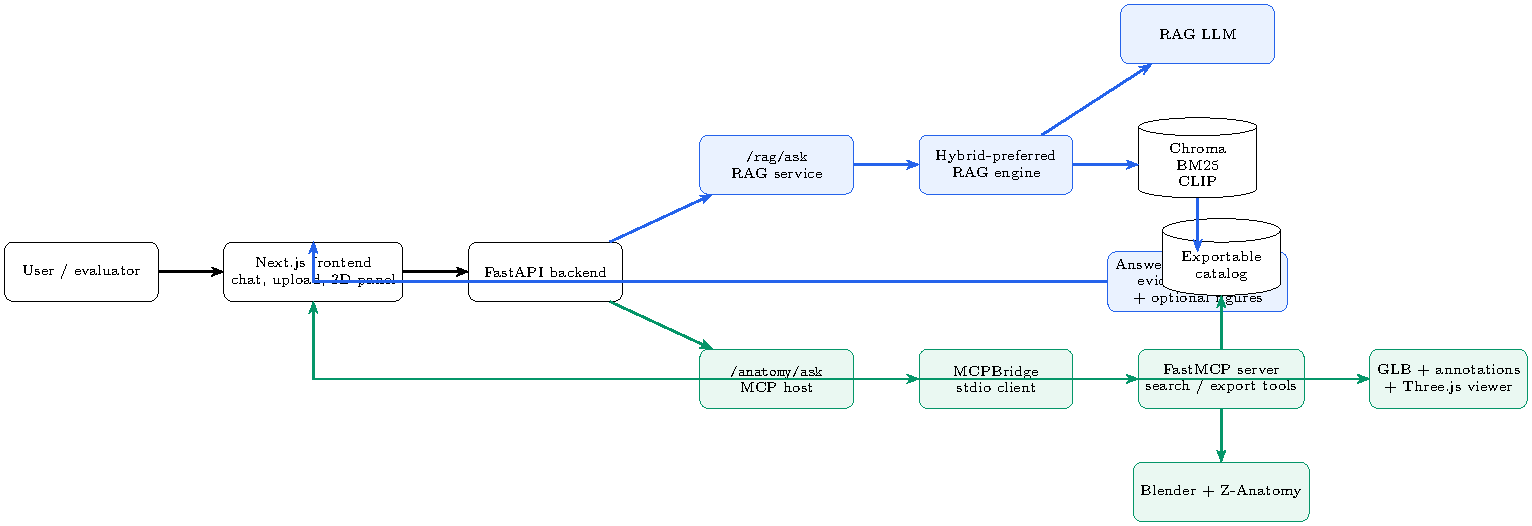
\includegraphics[
    width=\textwidth,
    height=0.64\textheight,
    keepaspectratio
  ]{figures/rendered/dual_pipeline_architecture.pdf}
  \caption{High-level dual-pipeline architecture of the anatomy learning assistant. The document path uses uploaded PDFs with hybrid-preferred retrieval and returns an answer with question-type-capped evidence context and optional figures. The three-dimensional path uses a validated anatomy catalogue and controlled export tools to return an inspectable model artefact.}
  \label{fig:dual-pipeline-intro}
\end{figure}

\Cref{fig:dual-pipeline-intro} shows the division of responsibility. In document mode, passages and optional figures are retrieved before the answer and source metadata are returned. In 3D mode, a structure is resolved against a catalogue and an external export tool is invoked. The evaluation follows the same division: document responses are examined through evidence and citation behaviour, whereas 3D responses require a tool trace and an accessible artefact.

\section{Thesis Structure}
\label{sec:introduction-structure}

\Cref{chap:background} introduces the theoretical and technical foundations. \Cref{chap:methodology} explains the research approach, requirements, constraints, and evidence boundaries. \Cref{chap:evolution} reconstructs the decisions that shaped the prototype, and \cref{chap:implementation} maps the final architecture to the archived code. \Cref{chap:evaluation} describes what was and was not evaluated. Results and limitations are discussed in \cref{chap:results}; \cref{chap:conclusion} then answers the research questions and prioritises the remaining work.

\chapter{Background and Related Work}
\label{chap:background}

\begin{chapterplan}{14--17 pages}{Establish the scientific foundations for the thesis design and position the work relative to prior research without prematurely describing the implementation.}
The review connects educational language models with document retrieval, multimodal evidence, 3D anatomy, and tool execution. It also marks the point at which the literature stops and project-specific evidence must begin.
\end{chapterplan}

The prototype combines ideas that are usually evaluated separately. Its document route relies on educational language models, information retrieval, grounding, and multimodal search. Its 3D route depends on anatomy visualisation, browser graphics, tool-using models, and the Model Context Protocol (MCP). The purpose of this chapter is to establish those foundations and to show why they lead to different verification requirements.

This is a structured narrative review rather than a systematic review. I recorded sources in a literature matrix and prioritised canonical method papers, recent peer-reviewed evaluations, and official specifications. The review can therefore support the design argument and define relevant concepts. It cannot demonstrate that no comparable system exists, and it is not evidence that the implementation works.

\section{Large Language Models in Education}
\label{sec:llms-education}

A conversational model can explain, reformulate, summarise, answer questions, and generate feedback. In educational settings, this is attractive because a learner can ask for help without knowing the heading or terminology used by a textbook. Reviews describe opportunities for personalised interaction and teacher support, but they also show that educational value depends on the task, the quality of feedback, and the surrounding pedagogy \parencite{kasneci2023}.

Anatomy provides a plausible use case because students regularly move between names, functions, spatial relationships, and visual representations. They may want a pathway explained in smaller steps or need help comparing two structures. A conversational interface can support that exploration, but it does not turn the model into an authoritative source. A systematic review of LLMs in medical education found broad use across learning and assessment tasks alongside accuracy concerns and large differences in models, prompts, and evaluation methods \parencite{lucas2024medicaleducation}.

The main risks are not limited to wrong facts. Bias, privacy exposure, over-reliance, and reduced critical engagement have also been discussed \parencite{kasneci2023,lucas2024medicaleducation}. Fluent wording can make unsupported content difficult to identify \parencite{ji2023}. In anatomy, a small lexical difference may alter the answer materially: left and right, a closely related structure name, or the distinction between a nerve and a vessel.

Learning support and assessment should also be separated. A model may help a student explore a concept, but the generated explanation is not evidence of unaided mastery unless the assessment design accounts for the assistance. Institutions must additionally consider retention of student data, copyright-sensitive teaching material, transparency, and responsibility for errors. These concerns shaped the present project: the interface should be tied to an identifiable knowledge source, missing support should remain visible, and the tool should complement rather than replace expert teaching. Any claim about learning outcomes would require a separate study.

\section{Hallucination, Factuality, Grounding, and Provenance}
\label{sec:hallucination-grounding}

The term \emph{hallucination} is used in several ways. Here it covers generated content that lacks support in the relevant source, conflicts with the supplied input, or is factually wrong relative to accepted external knowledge \parencite{ji2023,wang2024factuality}. This definition contains two questions that should not be collapsed. \emph{Faithfulness} concerns the relationship between the answer and the context given to the model. \emph{Factuality} concerns agreement with external knowledge. An answer can be faithful to an incorrect document, or factually correct while unsupported by the documents the user asked the system to use.

Grounding and provenance describe different parts of the evidence chain. Grounding is the support relationship between a claim and evidence. Provenance identifies where that evidence came from, such as a PDF, page, and passage. A citation is the reference shown to the user. Retrieval, grounding, provenance, and citation are therefore connected stages rather than interchangeable terms.

Unsupported generation can arise from incomplete or conflicting pre-training data, an ambiguous prompt, weak retrieved context, or a decoding process that favours a plausible continuation over an admission of uncertainty \parencite{ji2023,wang2024factuality}. Retrieval supplies external information at inference time, but the generator may still ignore it, extend it, or attach it to the wrong claim. RAGTruth provides fine-grained evidence that hallucination remains present even when retrieved context is available \parencite{niu2024ragtruth}.

Mitigation methods work at different layers. Fine-tuning, calibration, and self-critique act on or around the model. Application controls include retrieval, constrained prompts, external verification, citation checks, and abstention \parencite{ji2023,wang2024factuality}. None of these controls covers the whole route. For a document-grounded application, a practical strategy is to retain passage identifiers and inspect whether each substantive claim is supported by the material shown to the model.

Scores need the same discipline. A confident tone is not evidence of confidence, and a similarity score is not an anatomy-correctness probability. The evaluation must keep passage retrieval, answer faithfulness, citation support, and independent anatomical correctness visible as separate constructs.

\section{Retrieval-Augmented Generation}
\label{sec:rag-background}

Retrieval-augmented generation combines a generative model with an external collection. In the foundational formulation, retrieved documents serve as non-parametric memory alongside knowledge encoded in model parameters \parencite{lewis2020}. A practical RAG system usually has two phases. During ingestion, documents are extracted, divided into passages, represented, and stored with metadata. At query time, candidates are retrieved and ranked before selected evidence is supplied to the generator.

Much of the quality is determined before the LLM receives a prompt. Scanned pages may require OCR; multi-column layouts may be extracted in the wrong order; chunks may be too short to preserve an explanation or too long to isolate the relevant statement. Repeated ingestion can create duplicate records. Source and page metadata must survive these stages if the interface is expected to show provenance. Such choices are part of the method rather than neutral preprocessing \parencite{xiong2024medrag}.

For educational documents, RAG offers three practical advantages. The corpus can change without retraining the generator, retrieved passages can be shown to the user, and local or course-specific material can be prioritised over broad parametric knowledge \parencite{lewis2020}. The same architecture can support abstention when evidence is weak, but only if the application checks sufficiency instead of assuming that the top-ranked passage is adequate.

There is no single standard pipeline. Extraction, chunking, query processing, retrieval, ranking, context construction, and generation all affect the result. Medical RAG benchmarks show interactions between the corpus, retriever, and language model \parencite{xiong2024medrag}. Self-RAG takes another approach by learning when to retrieve and critique evidence rather than treating retrieval as a fixed preliminary step \parencite{asai2024selfrag}. That additional control comes with greater training and orchestration complexity.

For this thesis, a modular design was methodologically useful. Individual stages could be inspected and replaced without hiding their behaviour inside a larger learned controller. The evaluation still had to follow the components. A retrieval miss, irrelevant context, source conflict, prompt limitation, and unsupported synthesis may all end in a poor answer, but they require different corrections.

\section{Sentence Embeddings, MiniLM, and Dense Retrieval}
\label{sec:dense-retrieval-background}

Dense retrieval represents questions and passages as vectors and ranks passages by proximity in a shared space. Sentence-BERT uses Siamese or triplet architectures to produce sentence embeddings that can be compared efficiently \parencite{reimers2019}. Dense Passage Retrieval uses separate question and passage encoders so that document vectors can be prepared before a query arrives \parencite{karpukhin2020}. Both methods support semantic matching when the learner's wording differs from the wording in the source.

MiniLM reduces Transformer size through knowledge distillation while retaining useful representation capacity \parencite{wang2020}. MiniLM-based Sentence-Transformers are widely used in resource-constrained retrieval systems. Reproducible reporting still requires the exact model card, dimensionality, objective, and licence \parencite{minilmModelCard}.

Query and passage vectors are commonly compared with cosine similarity. A vector store can retain the vector together with the original passage and its metadata, while an approximate nearest-neighbour index makes search efficient. The returned value describes proximity under the selected model and distance function. It is not a probability that the passage answers the question and should not be presented as factual confidence \parencite{reimers2019,minilmModelCard}.

Dense retrieval is well suited to paraphrases, although performance varies across domains and datasets \parencite{thakur2021beir}. Exact labels, abbreviations, and laterality may still be decisive. Anatomy shows the trade-off clearly: semantic similarity helps when a student paraphrases a function, whereas tokens such as \emph{left}, \emph{right}, or a Latin name may need exact preservation. This motivates adding a lexical signal rather than replacing semantic retrieval altogether.

\section{BM25, Sparse Retrieval, Hybrid Retrieval, and Reciprocal Rank Fusion}
\label{sec:hybrid-retrieval-background}

Sparse retrieval ranks documents from lexical evidence. BM25 rewards occurrence of query terms, gives more weight to discriminative terms, applies term-frequency saturation, and normalises for document length \parencite{robertson2009}. One common formulation is

\begin{equation}
\mathrm{BM25}(q,d)=\sum_{t\in q}\mathrm{IDF}(t)
\frac{f(t,d)(k_1+1)}{f(t,d)+k_1\left(1-b+b\frac{|d|}{\mathrm{avgdl}}\right)},
\label{eq:bm25}
\end{equation}

where $f(t,d)$ is the frequency of term $t$ in document $d$, $|d|$ is the document length, $\mathrm{avgdl}$ is the average document length, and $k_1$ and $b$ control saturation and length normalisation. BM25 is useful for exact structure names, abbreviations, numerical expressions, and laterality. Its weakness is vocabulary mismatch: a relevant passage may express the same idea with different words.

Dense and sparse search therefore contribute different signals. A hybrid retriever can gather candidates from both rankings. Directly averaging raw scores is problematic because cosine similarity and BM25 values are on different scales. Reciprocal Rank Fusion (RRF) uses positions instead \parencite{cormack2009}:

\begin{equation}
\mathrm{RRF}(d)=\sum_{r\in R}\frac{1}{k+\mathrm{rank}_{r}(d)},
\label{eq:rrf}
\end{equation}

where $R$ is the set of rankings and $k$ limits the influence of large rank differences. A passage can contribute strongly when either retriever places it near the top.

Fusion is usually followed by further control. Reranking examines a smaller candidate pool against the exact question, while deduplication prevents overlapping chunks, repeated pages, or repeated ingestion from dominating the context. Neither step establishes that the evidence is sufficient. A passage may be highly related to the topic and still omit the statement required for the answer.

Hybrid retrieval also adds operational and methodological costs. Lexical search can over-rank passages that repeat a term without addressing the question, and the sparse index must remain synchronised with the vector store. Fusion weights, query rewriting, and reranking introduce choices that need validation. In this thesis, dense-plus-BM25 retrieval is treated as a testable design hypothesis rather than an assumed improvement.

\section{CLIP and Multimodal Retrieval}
\label{sec:clip-multimodal}

Contrastive Language--Image Pre-training (CLIP) learns text and image encoders in a shared space from paired image--text data \parencite{radford2021}. Training pulls matched pairs closer and separates unrelated pairs. Once image embeddings have been computed, a textual query can be compared with them, which enables text-to-image retrieval without a separate classifier for every visual category.

This is relevant to anatomy because useful evidence may appear in diagrams, radiographs, histology, screenshots, or cross-sectional figures. Retrieval is preferable to image generation when the aim is to return material from an uploaded source and preserve its provenance. General CLIP models were trained on broad web data and may miss specialised biomedical distinctions. MedCLIP adapts contrastive learning to medical image--text data \parencite{wang2022medclip}, but a model trained on clinical images is not automatically ideal for textbook pages that combine drawings, labels, screenshots, and photographs.

Model selection therefore requires representative evaluation rather than a domain label alone. MiniLM and CLIP scores also have no common numerical meaning because the models were trained with different objectives and in different spaces \parencite{reimers2019,radford2021}. Late fusion is easier to audit: text and images are retrieved independently and joined only in the response.

Captions, page metadata, and nearby text may improve image search, but PDF extraction can associate the wrong text with a figure or split a composite image. Decorative images, duplicates, small labels, broken URLs, and fine anatomical relations add further failure modes. Image availability and visual relevance need their own measures. A learner study would still be required before claiming that the returned figures improve learning.

\section{Evaluation of Retrieval-Augmented Generation}
\label{sec:rag-evaluation-background}

An end-to-end RAG score can hide the point of failure. The evidence may never have been retrieved; a useful passage may have been ranked too low; the generator may have ignored the context; or a source may have been attached to the wrong claim. Frameworks such as RAGAS, ARES, and RAGChecker reflect this modularity by evaluating context, answers, and support separately \parencite{es2024ragas,saadfalcon2024ares,ru2024ragchecker}.

Automated evaluators add another model- and prompt-dependent layer. Their agreement with human judgement should be checked in the target domain rather than assumed. ARES and RAGChecker include meta-evaluation against human annotations \parencite{saadfalcon2024ares,ru2024ragchecker}. For anatomy, an expert-labelled subset can also check laterality, structural relationships, and whether an explanation is educationally adequate. Raw outputs should be preserved so later reviewers can revisit the scoring.

\subsection{Retrieval effectiveness}

Let $R_q$ be the set of passages judged relevant for question $q$, and let $D_q^{(k)}$ be the first $k$ retrieved passages. Precision at $k$ measures how many returned passages are relevant, while Recall at $k$ measures how much of the known relevant set was recovered:

\begin{equation}
\mathrm{Precision@}k=\frac{|D_q^{(k)}\cap R_q|}{k},
\qquad
\mathrm{Recall@}k=\frac{|D_q^{(k)}\cap R_q|}{|R_q|}.
\label{eq:precision-recall-k}
\end{equation}

Mean Reciprocal Rank (MRR) focuses on the first relevant result and assigns zero when none is retrieved:

\begin{equation}
\mathrm{MRR}=\frac{1}{N}\sum_{q=1}^{N}\frac{1}{\mathrm{rank}_q}.
\label{eq:mrr}
\end{equation}

Reciprocal rank appeared in early question-answering evaluation, including TREC-8 \parencite{voorhees1999}. It is informative when one strong passage can answer a question, but it ignores further relevant passages. Normalised Discounted Cumulative Gain (nDCG) supports graded relevance and rewards useful material near the top \parencite{jarvelin2002}:

\begin{equation}
\mathrm{DCG@}k=\sum_{i=1}^{k}\frac{2^{rel_i}-1}{\log_2(i+1)},
\qquad
\mathrm{nDCG@}k=\frac{\mathrm{DCG@}k}{\mathrm{IDCG@}k}.
\label{eq:ndcg}
\end{equation}

All three measures depend on the relevance judgements. If the gold set contains only one acceptable passage when several could support the answer, recall and nDCG may understate retrieval quality.

\subsection{Answer quality, faithfulness, and citations}

Correctness concerns agreement with an expert answer or accepted reference. Completeness asks whether the necessary aspects were covered. A short response may be correct but incomplete; a detailed response may include the required information and still introduce unsupported claims. Lexical overlap alone is therefore a weak measure for free-form explanations.

Faithfulness is assessed against the context supplied to the generator. One practical approach is to divide an answer into substantive claims and label each claim as supported, partly supported, unsupported, or contradicted. RAGTruth illustrates the value of fine-grained annotation for hallucination in retrieved-context generation \parencite{niu2024ragtruth}. The following ratio makes the intended construct explicit:

\begin{equation}
\mathrm{Hallucination\ Rate}=
\frac{\text{unsupported or contradicted claims}}
{\text{all substantive claims}}.
\label{eq:hallucination-rate}
\end{equation}

The annotation protocol must specify how claims are segmented and how partial support is counted. A system can also reduce the ratio by making fewer claims, so hallucination and completeness should be interpreted together.

Citations are valuable only when they support the attached statement. ALCE separates citation correctness from citation completeness \parencite{gao2023alce}. Correctness asks whether the cited passage supports the claim; completeness asks whether all claims that require evidence are cited. Exact quotation adds a stricter condition: the displayed wording must match the source and page. A paraphrase should not be labelled as a quotation.

\subsection{Boundary and multimodal evaluation}

A document-constrained assistant should sometimes refuse, qualify, or ask for clarification. Unsupported, off-topic, ambiguous, typo-containing, and quotation requests test whether the system recognises the limits of its corpus. False acceptance occurs when it answers without adequate evidence; false rejection occurs when it refuses despite sufficient support. If general knowledge is permitted, the interface should identify that basis explicitly.

Images require a parallel evaluation. Top-1 relevance, Precision@$k$, duplicate rate, broken-URL rate, source-page accuracy, and image--answer consistency cannot be inferred from text quality. A defensible RAG study therefore combines retrieval measures with human or validated model-assisted answer review, citation checks, boundary cases, and separate operational and visual tests.

\section{Three-Dimensional Anatomy Education and Browser-Based Visualisation}
\label{sec:3d-anatomy-education}

Anatomy requires reasoning about depth, orientation, and relationships that are difficult to express in one two-dimensional view. Interactive models permit rotation, zooming, isolation, and inspection from several perspectives. \textcite{yammine2015} reported benefits for factual and spatial anatomy knowledge, while reviews of virtual and augmented reality found potential advantages alongside wide variation in study quality, instructional design, and hardware \parencite{moro2017,garciarobles2024}.

Engagement and novelty are not learning outcomes. Immersive hardware may introduce cost, discomfort, and access barriers, and a preferred interface may not improve retention \parencite{moro2017,garciarobles2024}. Browser delivery avoids specialist headsets and suits an initial feasibility study whose immediate question is whether a requested structure can be delivered and inspected reliably.

Three-dimensional resources remain complementary to cadaveric, clinical, and conventional teaching. Their effectiveness depends on the learning task, guidance, asset quality, and integration with the curriculum \parencite{yammine2015,moro2017,garciarobles2024}. Earlier work demonstrated browser-based interactive anatomy visualisation \parencite{petersson2009}. glTF provides a runtime format, and GLB can package the scene into one binary asset \parencite{khronosGltf}. Loading a model successfully, however, does not prove that the correct structure was selected. Source, selection, export, and viewer behaviour all remain part of the evidence chain.

\section{Tool-Using Large Language Models}
\label{sec:tool-using-llms}

Tool-using language-model systems allow a model to request an operation that is executed outside the model. The model interprets the user's wording and proposes a tool with structured arguments; external software performs the action. This pattern is relevant when the desired result is a database query, calculation, retrieval operation, or file rather than prose alone.

ReAct interleaves reasoning, actions, and observations \parencite{yao2023react}. Toolformer studies self-supervised insertion of API calls \parencite{schick2023toolformer}, while ToolLLM addresses training and evaluation over a large set of real-world APIs \parencite{qin2024toolllm}. These approaches establish tool choice and tool use as capabilities distinct from ordinary text generation. They also make the result of an external operation observable.

Schemas form a contract between the model-facing host and the tool. Required fields can be validated, and a trace can retain the selected operation, arguments, status, result, and error. A valid call is only the first step. The model may choose the wrong tool, supply invalid arguments, repeat calls, or misread the result. The tool may fail because of permissions, configuration, missing resources, or timeouts.

When an operation has side effects, the host should validate the result and expose failure clearly. Bounded tools are easier to audit than unrestricted code execution. That principle motivates the separation in this thesis between interpreting an anatomy request and exporting a 3D structure. The cited work motivates tool-mediated action; MCP supplies the communication protocol used in the implementation.

\section{Model Context Protocol as a Technical Protocol}
\label{sec:mcp-background}

MCP is an open protocol for communication between AI applications and capability servers. It defines host, client, and server roles over JSON-RPC. The host coordinates interaction with the user and model, the client maintains the protocol session, and the server exposes tools, resources, or prompts \parencite{mcp20251125}. MCP standardises discovery, schemas, lifecycle negotiation, messages, results, and transport. It leaves the host's reasoning strategy and model choice open.

A tool is described by a name, purpose, and input schema. The client can list available tools and invoke one with structured arguments; the server can return structured and textual content \parencite{mcp20251125}. In a 3D export workflow, the structured result may include status, a canonical structure label, model and annotation URLs, and an explicit error. The host can inspect those fields before reporting success.

Stdio is one supported transport. The client launches a server subprocess and exchanges JSON-RPC messages through standard input and output. Streamable HTTP supports networked deployment \parencite{mcp20251125}. Protocol versions are negotiated during initialisation. The 2025-06-18 and 2025-11-25 revisions show why a reproducible study must record both the specification and the SDK version used by the frozen runtime \parencite{mcp20250618,mcp20251125}.

Versioning matters because tool definitions, transports, and SDK interfaces can change. MCP improves interoperability and gives the host structured evidence of a call, but permissions, input validation, result checks, and context exposure remain host responsibilities \parencite{mcp20251125}. In this project, correct output also depends on resolving the intended structure, selecting appropriate source geometry, exporting a valid model, and loading it in the viewer.

\section{Positioning of This Thesis}
\label{sec:positioning-thesis}

The literature supplies established methods for each part of the prototype. Educational LLM research explains both the attraction and the risks of conversational interaction. Information retrieval and RAG support document-conditioned answers. Vision--language models enable retrieval of existing figures. Anatomy-education research motivates spatial resources, and tool-use research separates language interpretation from external action. MCP provides the protocol boundary for that action.

The thesis does not introduce a new foundation model, retrieval algorithm, vision encoder, or protocol. Its contribution lies in integration and evidence: how can these methods be combined while preserving different verification rules for document claims and 3D artefacts? \Cref{tab:related-work-comparison} summarises that position.

\begin{small}
\begin{longtable}{@{}L{0.15\textwidth} L{0.18\textwidth} L{0.275\textwidth} L{0.275\textwidth}@{}}
\caption{Comparison of representative related work and the scope of this thesis.}
\label{tab:related-work-comparison}\\
\toprule
Area & Representative work & Established contribution & Relationship to this thesis \\
\midrule
\endfirsthead
\multicolumn{4}{c}{\tablename\ \thetable{} -- continued}\\
\toprule
Area & Representative work & Established contribution & Relationship to this thesis \\
\midrule
\endhead
\midrule
\multicolumn{4}{r}{Continued on next page}\\
\endfoot
\bottomrule
\endlastfoot
Educational LLMs & \textcite{kasneci2023}; \textcite{lucas2024medicaleducation} & Conversational support and documented educational risks & Motivates constrained interaction; no learning-outcome claim \\
Hallucination and RAG & \textcite{ji2023}; \textcite{lewis2020}; \textcite{xiong2024medrag} & Hallucination taxonomy and external-evidence generation & Motivates grounding, provenance, and component-level evaluation \\
Dense retrieval & \textcite{reimers2019}; \textcite{karpukhin2020} & Efficient semantic representations and passage retrieval & Supports paraphrase-sensitive document search \\
Sparse and hybrid retrieval & \textcite{robertson2009}; \textcite{cormack2009} & Exact lexical matching and rank-based fusion & Motivates testable BM25+dense retrieval for anatomy terms \\
Multimodal retrieval & \textcite{radford2021}; \textcite{wang2022medclip} & Contrastive text--image alignment & Supports retrieval of existing PDF figures, not image generation \\
RAG evaluation & \textcite{es2024ragas}; \textcite{gao2023alce}; \textcite{saadfalcon2024ares} & Context, faithfulness, answer, and citation evaluation & Informs separate retrieval, grounding, citation, and boundary metrics \\
3D anatomy education & \textcite{yammine2015}; \textcite{garciarobles2024} & Conditional evidence for spatial and factual learning support & Motivates browser-based 3D support; effectiveness needs a user study \\
Tool-using LLMs & \textcite{yao2023react}; \textcite{schick2023toolformer}; \textcite{qin2024toolllm} & Models that select and invoke external actions & Motivates verifiable execution rather than prompt-only claims \\
MCP & MCP specifications \parencite{mcp20250618,mcp20251125} & Host--client--server communication, schemas, and transports & Defines the protocol boundary for local search and export tools \\
\end{longtable}
\end{small}

Most of the reviewed work studies document grounding, image retrieval, 3D anatomy, and tool execution as separate problems. This thesis preserves that separation inside one prototype. Document claims are examined against retrieved sources; 3D success is tied to resolution and observable artefacts. The position is deliberately narrower than clinical correctness, production readiness, or demonstrated learning improvement. \Cref{chap:methodology} translates these foundations into the research approach and requirements.

% Target file: chapters/03_methodology_requirements.tex
%
% This chapter requires the following verified bibliography keys:
% iso29148, iso25010, eu2016gdpr, eu2001infosoc, pineau2021
%
% It also expects the following rendered figure:
% figures/rendered/research_cycle.pdf

\chapter{Research Methodology and Requirements}
\label{chap:methodology}

\begin{chapterplan}
  {8--10 pages}
  {Justify the research approach, describe the iterative process, derive testable requirements, and connect the research questions to artefact components and experiments.}
Primary evidence: design-science literature, the archived repository, supervisor traceability records, project design documents, formative evaluations, and reproducibility records.
\end{chapterplan}

\section{Introduction}
\label{sec:methodology-introduction}

The focus here is the way the project was investigated. Implementation details are deferred to \cref{chap:implementation}; this chapter instead explains the research approach, reconstructs the development sequence, and converts broad project aims into requirements that can be checked. I follow the principle in ISO/IEC/IEEE 29148 that a requirement should state observable behaviour together with a means of verification \parencite{iso29148}.

Although the two modes share the same application shell, they answer different technical questions. Document mode ingests anatomy PDFs and may return an answer, source records, and figures. The 3D mode resolves a structure against a geometry-oriented catalogue and uses an MCP toolchain to invoke Blender, producing a GLB, annotations, and a viewer URL. I keep their sources, failure modes, and evidence separate throughout the method because combining them would make later results difficult to interpret.

The requirements changed as the prototype changed. Research questions and supervisor feedback supplied the initial direction, while repository inspection and formative use exposed requirements that had not been visible at the outset.
\footnote{Project evidence: \codepath{project_resources/ARCHITECTURE_FOR_DIAGRAMS.md}, \codepath{project_resources/THESIS_SYSTEM_DESIGN_AND_MCP.md}, \codepath{project_resources/PROFESSOR_REQUIREMENTS_TRACEABILITY.md}, and \codepath{project_resources/EVALUATION_DATA_SUMMARY.md}.}

\section{Research Approach and Justification}
\label{sec:research-approach}

\subsection{Design-Science Orientation}
\label{subsec:design-science-orientation}

The research problem is constructive: the study asks how an anatomy assistant can be built so that document answers remain traceable and 3D actions leave inspectable evidence. A design-science orientation fits this problem because building and evaluating the artefact generates knowledge about both the proposed intervention and the setting in which it is used \parencite{hevner2004}.

The six activities described by \textcite{peffers2007} can be recognised in the project, but they did not occur as one orderly sequence. Demonstrations repeatedly sent the work back to design: exact terminology was missed, references were duplicated, local asset paths failed away from the development machine, and the first Blender outputs had weak anatomy provenance. Each problem changed either the artefact or the standard used to judge it. This iterative pattern is close to Wieringa's distinction between designing a treatment and investigating its behaviour in context \parencite{wieringa2014}.

\begin{figure}[htbp]
  \centering
  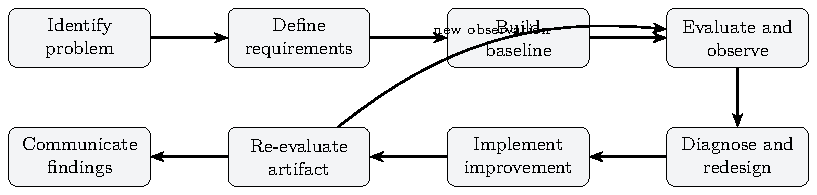
\includegraphics[
    width=0.74\textwidth,
    height=0.32\textheight,
    keepaspectratio
  ]{figures/rendered/research_cycle.pdf}
  \caption{Iterative design-science process used in the project. Formative observations generated revised requirements before final evaluation.}
  \label{fig:research-cycle}
\end{figure}

\subsection{Artefact, Evaluation Object, and Boundaries}
\label{subsec:artifact-evaluation-boundaries}

The artefact extends beyond the chat interface. It includes PDF ingestion, text and image indexes, retrieval and generation services, storage handling, the MCP host and client, the anatomy tool server, the export catalogue, Blender scripts, generated files, and the browser viewer.
\footnote{Project evidence: \codepath{project_resources/THESIS_SYSTEM_DESIGN_AND_MCP.md}; implementation locations are mapped in \cref{chap:implementation}.}
The evaluation object is their behaviour during defined tasks: ordinary anatomy questions, unsupported requests, ambiguous structure names, and selected technical failures.

The intended contribution has three parts: the dual-pipeline artefact, the measurements and failure cases retained from evaluation, and the engineering knowledge gained from designs that were kept, revised, or abandoned. These claims require different evidence. A class or endpoint can show that something was implemented; improvement requires a comparison and a recorded outcome \parencite{hevner2004,wieringa2014}.

The study remains a prototype investigation. It can examine retrieval, source linkage, figure delivery, catalogue resolution, artefact generation, and error handling. It was not designed to establish clinical validity or learning outcomes. In an educational anatomy setting, that limitation matters because fluent errors and over-reliance can affect learners who are not yet able to challenge the system \parencite{ji2023,kasneci2023}.

\section{Actual Iterative Research Process}
\label{sec:research-process}

The first working baseline used dense document retrieval. PDF text was chunked, embedded, stored in Chroma, and passed to a language model after similarity search. That simple route was useful because its weaknesses appeared quickly: exact terms were missed, repeated chunks crowded the source list, weak passages supported confident answers, and image-heavy material was poorly represented.
\footnote{Project evidence: \codepath{project_resources/THESIS_RESEARCH_LOG.docx} and \codepath{project_resources/EVALUATION_DATA_SUMMARY.md}.}

The next changes were incremental rather than a complete rewrite. Dense retrieval was retained for semantic matching, while BM25 and phrase matching were added to preserve lexical evidence. RRF combined the rankings without treating dense and sparse scores as directly comparable \parencite{robertson2009,cormack2009}. Text fingerprints and source--page checks addressed repeated passages. An earlier hard three-source cap came from a usability problem---crowded evidence cards---rather than from an optimisation study. Evidence grading, constrained prompts, citation filtering, and abstention were developed later when it became clear that topical similarity alone was not enough.

Figures could not be handled as a small extension to the text index. They were extracted, linked to metadata, and indexed through CLIP for text-to-image search \parencite{radford2021}. Once images were returned to the interface, the method also had to consider uniqueness, relevance, source traceability, and whether the browser could load the URL. Text-answer metrics could not answer those questions.

The 3D branch changed for comparable reasons. Procedural Blender output and fixed previews confirmed that subprocess execution worked, but they did not provide a general export grounded in an anatomy source. Z-Anatomy became the scene source, the raw label index was replaced by \codepath{exportable_catalog.json}, and direct Python calls moved behind an MCP client and server. With stdio transport, the client launches the server and exchanges JSON-RPC messages through standard input and output \parencite{mcp20250618}. The acceptance rule changed at the same time: assistant prose was no longer enough; the host needed structured tool output and an accessible artefact.

Before measurement, the intended final step was to freeze code, data, prompts, models, retrieval settings, Blender, the catalogue, the operating system, and hardware. Such records are central to reproducible machine-learning research \parencite{pineau2021}. The July run did not preserve the complete set together. I therefore use the formative spreadsheets as design evidence and restrict final claims to responses and artefacts that can still be traced.

\subsection{Verified production document route}
\label{subsec:verified-production-route}

Call-path inspection of the post-\texttt{5089fcc} production bundle in \codepath{src/multimodal/multimodal_rag_chain.py} shows that the hybrid-preferred route used by the primary English evaluation proceeds as follows:

\begin{enumerate}[leftmargin=*,itemsep=0.15em,topsep=0.3em]
  \item classify the question type;
  \item rewrite queries (typo correction and expansion where available);
  \item invoke \codepath{HybridRetriever};
  \item generate dense, BM25, and phrase candidates;
  \item fuse candidate rankings with Reciprocal Rank Fusion;
  \item apply source-aware deduplication (text fingerprint and normalised source--page keys);
  \item rerank surviving passages;
  \item apply pre-generation evidence filtering;
  \item select a question-type-dependent final context (approximately four to eight passages); and
  \item generate the answer and return source records, with optional CLIP figure objects.
\end{enumerate}

Dense similarity search remains only as a fallback if hybrid construction or search fails. Metric definitions, denominators, and proxy thresholds are stated in \cref{chap:evaluation}; this chapter records the process that was built, not the scores.

\section{Requirements Derivation and Evidence}
\label{sec:requirements-derivation}

Five sources informed the requirements: the research questions, supervisor comments, architecture records, the research log, and formative evaluation data. ISO/IEC/IEEE 29148 guided the phrasing of verifiable statements, while ISO/IEC 25010 supplied terminology for reliability, security, maintainability, usability, portability, and performance \parencite{iso29148,iso25010}.

The tables use four evidence codes:

\begin{itemize}[leftmargin=*,nosep]
  \item \textbf{S -- supervisor traceability:} design alternatives, failures, local and copyright concerns, source selection, reference limits, and broader anatomy-structure testing;
  \item \textbf{A -- architecture and system-design records:} separate RAG and MCP routes, sources, outputs, tools, and evaluation criteria;
  \item \textbf{L -- research log:} image-heavy retrieval, duplicate passages, URL delivery, grounding limits, and candidate caps; and
  \item \textbf{E -- evaluation summary:} quotation, typo, citation-relevance, boundary, and weak-evidence failures, together with the formative status of current scores.
\end{itemize}

These records explain how the requirements arose. They do not replace call-path inspection or final experiments.

\section{Functional Requirements}
\label{sec:functional-requirements}

The functional requirements in \cref{tab:functional-requirements} state the observable operations needed for RQ1--RQ3 and for the evidence used in RQ4. A route or class shows that a feature was implemented; compliance depends on the corresponding verification criterion.

{\scriptsize
\setlength{\tabcolsep}{3pt}
\renewcommand{\arraystretch}{1.00}
\begin{table}[htbp]
  \centering
  \caption{Functional requirements and verification criteria.}
  \label{tab:functional-requirements}
  \begin{tabularx}{\textwidth}{L{0.07\textwidth} Y Y L{0.11\textwidth}}
    \toprule
    ID & Requirement & Verification & Evidence \\
    \midrule
    FR1 &
    Accept anatomy PDFs through the interface or API. &
    Valid input returns ingestion status; invalid input returns an error. &
    S, A \\

    FR2 &
    Index usable text with document and page metadata. &
    Retrieved chunks retain source identity and page information. &
    S, L \\

    FR3 &
    Extract and index figures where technically possible. &
    Figure records contain context, storage location, and index metadata. &
    S, L \\

    FR4 &
    Answer document questions using indexed evidence. &
    An answer contains inspectable evidence or an explicit no-evidence state. &
    S, E \\

    FR5 &
    Limit returned references to a compact, deduplicated evidence set. &
    Responses contain deduplicated source records under the active context policy (historically a hard three-source design; evaluated July route used question-type-dependent caps). &
    S, L \\

    FR6 &
    Distinguish grounded, unsupported, and permitted world-knowledge output. &
    Unsupported requests abstain, ask for clarification, or disclose the boundary. &
    S, E \\

    FR7 &
    Return zero to three relevant figures when available. &
    URLs resolve, results are unique, and relevance is manually scored. &
    S, L \\

    FR8 &
    Expose RAG and MCP as separate user and API flows. &
    Each route uses only its intended source and output schema. &
    A \\

    FR9 &
    Resolve a structure expression to an exportable catalogue entry. &
    Exact, alias, laterality, and ambiguity tests produce expected outcomes. &
    S, A \\

    FR10 &
    Execute 3D search and export through discoverable MCP tools. &
    Tool discovery, calls, and tools used are recorded. &
    S, A \\

    FR11 &
    Return GLB, annotation, and viewer URLs after successful export. &
    Files are accessible, parseable, and visible in the viewer. &
    S, A \\

    FR12 &
    Suppress the success viewer when export evidence is incomplete. &
    A missing model URL, timeout, or tool error produces an explicit failure state. &
    S, A \\

    FR13 &
    Report readiness of critical dependencies. &
    Diagnostics identify missing models, storage, catalogue, MCP, or Blender. &
    S, A \\

    FR14 &
    Preserve final experiment inputs, outputs, configuration, and timing. &
    Every run maps to a revision, dataset version, raw record, and timestamp. &
    S, E \\
    \bottomrule
  \end{tabularx}
\end{table}
}

\section{Non-Functional Requirements}
\label{sec:nonfunctional-requirements}

The non-functional requirements adapt general software-quality concerns to the particular risks of source provenance and external tool execution \parencite{iso25010}. Performance appears as an obligation to measure latency, not as an unsupported claim that the prototype responds in real time.

{\scriptsize
\setlength{\tabcolsep}{3pt}
\renewcommand{\arraystretch}{1.00}
\begin{table}[htbp]
  \centering
  \caption{Non-functional requirements and verification criteria.}
  \label{tab:nonfunctional-requirements}
  \begin{tabularx}{\textwidth}{L{0.08\textwidth} Y Y L{0.11\textwidth}}
    \toprule
    ID & Requirement & Verification & Evidence \\
    \midrule
    NFR1 &
    Support institution-controlled storage of source and generated data. &
    The deployment record identifies local and external data flows. &
    S, A \\

    NFR2 &
    Minimise and control logs that may contain prompts or identifiers. &
    Logged fields, access, retention, and deletion are documented. &
    S \\

    NFR3 &
    Preserve source, version, permission, and licence provenance. &
    Corpus and asset manifests contain hashes and usage conditions. &
    S \\

    NFR4 &
    Keep RAG and MCP modular and independently testable. &
    Separate routes, services, tests, and outputs are available. &
    A \\

    NFR5 &
    Provide traceable results and explicit safe failures. &
    Sources or tool artefacts support success; failures identify the stage. &
    S, A \\

    NFR6 &
    Restrict MCP capabilities. &
    User input cannot select arbitrary blend files, paths, or code. &
    S, A \\

    NFR7 &
    Make final experiments reproducible. &
    Code, data, models, prompts, settings, hardware, and raw outputs are archived. &
    S, E \\

    NFR8 &
    Keep configuration portable and interface feedback understandable. &
    Environment-specific endpoints and paths are configurable; errors are actionable. &
    S, A \\

    NFR9 &
    Measure latency separately for RAG, cold export, and cached export. &
    Timings are reported per pipeline and condition. &
    S, A \\
    \bottomrule
  \end{tabularx}
\end{table}
}

\section{Local-First, Privacy, Copyright, and Deployment Constraints}
\label{sec:constraints}

I use \emph{local-first} to describe a data-control objective, not a guarantee of completely offline operation. PDFs, indexes, the Z-Anatomy source, the catalogue, Blender, and generated artefacts can remain on a developer- or institution-controlled machine. The repository also supports Groq and Supabase; when those services are enabled, passages or assets may leave the local environment.
\footnote{Code evidence: \codepath{src/llm/llm_factory.py}, \codepath{src/config/settings.py}, and \codepath{app/services/object_storage.py}.}
A strict locality claim requires local inference, controlled storage, and a reviewed telemetry path.

The technical tests did not require student identities or health data. Even so, questions, screenshots, uploaded files, and logs can contain personal information. Articles~5 and~25 GDPR make purpose limitation, minimisation, storage limitation, and data protection by design relevant when such data are processed \parencite{eu2016gdpr}. The practical response is to use synthetic identifiers, avoid retaining prompts without a reason, protect logs, define deletion, and inspect screenshots before publication. A later learner study would need a separate consent, ethics, and data-management procedure.

Copyright creates a different constraint. Local storage does not grant permission to reproduce or distribute a document. European Union law permits Member States to implement limited teaching and research exceptions, subject to conditions such as proportionality and source acknowledgement, but the applicable rule depends on national implementation and licence terms \parencite{eu2001infosoc}. The corpus should contain only authorised material. If a restricted PDF cannot be redistributed, the reproducibility package can retain its filename, hash, page references, and reconstruction instructions. The Z-Anatomy release, blend-file hash, licence, attribution, and derivative-export conditions require the same treatment \parencite{zanatomy}.

Running the prototype also depends on resources outside the application repository: a compatible Blender executable, the matching Z-Anatomy scene and catalogue, writable output locations, the MCP SDK, available embedding and generation models, persistent indexes, and URLs that the browser can reach.
\footnote{Project and code evidence: \codepath{src/config/settings.py}, \codepath{app/services/anatomy_mcp_service.py}, and \codepath{project_resources/ARCHITECTURE_FOR_DIAGRAMS.md}.}
They are included in RQ4 because they are part of the operational cost of local control.

\section{Assumptions and Non-Goals}
\label{sec:assumptions-nongoals}

The method assumes permission to use the selected PDFs and 3D assets, sufficient extractable text or figure content, and preservation of source and page metadata. It also assumes that the configured models remain available, Blender can open the selected Z-Anatomy file, and the catalogue corresponds to that scene version. The evaluation sets cover selected target behaviours rather than the full range of anatomy-learning questions.

The prototype is neither a diagnostic system nor a medical device or clinical decision-support tool. It excludes arbitrary Blender scripting and makes no guarantee of complete Z-Anatomy coverage or universal anatomical correctness. Learning gains require participants. Compact reference limiting is a design choice whose July form was type-dependent rather than a fixed three-source rule, and RAG and MCP are not collapsed into one confidence value. I describe a configuration as fully local only when external generation and storage services are disabled and that state is recorded.

\section{Research-Question Traceability and Evaluation Separation}
\label{sec:rq-traceability}

\Cref{tab:rq-traceability} links each research question to the artefact involved, the test or inspection performed, and the evidence carried into the results chapter. This mapping limits later interpretation to observations that were part of a defined procedure.

{\scriptsize
\setlength{\tabcolsep}{3pt}
\renewcommand{\arraystretch}{1.02}
\begin{table}[htbp]
  \centering
  \caption{RQ--artefact--experiment--evidence traceability matrix.}
  \label{tab:rq-traceability}
  \begin{tabularx}{\textwidth}{L{0.06\textwidth} L{0.23\textwidth} Y Y}
    \toprule
    RQ & Artefact & Experiment or Test & Evidence \\
    \midrule
    RQ1 &
    PDF ingestion, hybrid-preferred retrieval, answer generation, sources, and boundary handling &
    P1 English question set, automatic passage-ranking proxy, request outcomes, and boundary inspection &
    Precision@3, Recall@3, nDCG@3, MRR, completion counts, outcome classifications, and raw failure cases \\

    RQ2 &
    Figure extraction, CLIP index, and image URL publication &
    Image-object availability on the 10 figure-related P1 questions plus development observations &
    Image-object count and documented relevance limitations; no expert relevance or text-only baseline \\

    RQ3 &
    MCP host, client, server, catalogue, Blender export contract, and viewer &
    Repository and schema inspection of the success and failure conditions &
    Required tool trace, structured status, model URL, GLB, annotations, and explicit empirical limitations \\

    RQ4 &
    Complete local-first deployment and evaluation record &
    Cross-component design analysis, failure cases, dependency review, and reproducibility audit &
    Environment status, failure evidence, source-control observations, and qualitative trade-offs \\
    \bottomrule
  \end{tabularx}
\end{table}
}

A combined score would obscure the result. RAG is a question--retrieval--answer transaction, so the relevant evidence concerns passages, evidence use, citations, boundary behaviour, and figures. MCP is a query--tool--artefact transaction, which instead requires structure resolution, tool execution, file validity, viewer loading, and safe failure. The fixed-asset preview worker is excluded from MCP evaluation because it cannot perform arbitrary Z-Anatomy export. The completed evidence supports RQ3 as a verification design; runtime reliability and comparative effectiveness remain open.

\section{Ethical and Reproducibility Considerations}
\label{sec:ethics-reproducibility}

The assistant is intended as study support, not as a replacement for teaching material, educators, or clinical judgement. Users need visible evidence and limitations because fluent responses may still be unsupported \parencite{ji2023,kasneci2023}. An MCP trace similarly shows that an action occurred; it cannot by itself establish that the selected structure is anatomically correct. I retain failures in the research record rather than removing them from the analysis.

A reproducibility package should bring together the repository commit, environment, models, prompts, corpus and Z-Anatomy hashes, retrieval settings, evaluation versions, raw responses, tool results, generated artefacts, and timings \parencite{pineau2021}. Until the existing spreadsheets are reproduced under such a configuration, they remain formative records. AI-assisted drafting is disclosed in \cref{app:ai-disclosure}; the author remains responsible for the argument, source checks, analysis, and submitted wording.

The July evaluation did not preserve every required value. \Cref{app:reproducibility} therefore distinguishes reconstructable configuration from information that was not archived with the run.

\section{Chapter Summary}
\label{sec:methodology-summary}

The design-science framing reflects what happened in practice: building and demonstrating the system repeatedly changed the requirements. This chapter converted those requirements into observable checks and made the data-control, copyright, deployment, and reproducibility constraints explicit. It also mapped RQ1--RQ4 to the evidence available for each. RAG and MCP are separated methodologically as well as architecturally because they use different sources, produce different outputs, and require different units of analysis. \Cref{chap:evolution} traces the decisions that arose from the observed failures.

\chapter{System Evolution and Design Decisions}
\label{chap:evolution}

\begin{chapterplan}{14--17 pages}{Explain how the system changed in response to observed technical weaknesses, and distinguish implemented ideas from runtime behaviour and measured effects.}
The chapter reconstructs the main engineering decisions from project records and the archived repository. It reports what can be demonstrated and identifies where a proposed correction was not yet connected or evaluated.
\end{chapterplan}

\section{Purpose, Scope, and Evidence Standard}
\label{sec:evolution-purpose}

The architecture was not designed in one pass. It changed whenever the prototype exposed a practical problem. Dense vector search and procedural Blender output came first; lexical retrieval, deduplication, image search, storage abstraction, a geometry catalogue, and an MCP boundary followed later. Some of those changes became part of the active route, while others stopped at a branch or partial integration. I reconstruct that history because the unsuccessful and unfinished approaches explain the final design as much as the retained components do.

Rather than repeat a fixed checklist for every decision, I follow the sequence in which the problems became visible. The account asks what evidence was available at the time, why one correction was chosen, and what remained unresolved afterwards. That form of reflection is consistent with design-science research, where building and evaluating an artefact can produce knowledge about both the proposed solution and its context \parencite{hevner2004,peffers2007,wieringa2014}.

Four evidence levels are used. Project notes and formative evaluations support the historical account. Repository files show implementation. Call-graph inspection is required before a mechanism can be described as part of an endpoint, and a controlled run is required before any performance effect is claimed. The hybrid retriever is a useful example: the source code exists, but the archived production path did not instantiate it. Historical material comes mainly from \codepath{project_resources/THESIS_SYSTEM_DESIGN_AND_MCP.md}, \codepath{project_resources/EVALUATION_DATA_SUMMARY.md}, and \codepath{project_resources/PROFESSOR_REQUIREMENTS_TRACEABILITY.md}; implementation statements are checked against the repository.

\begin{figure}[htbp]
  \centering
  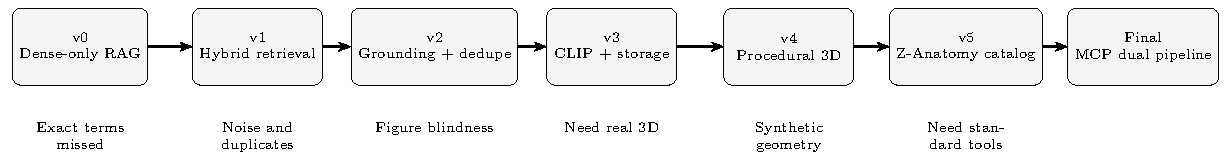
\includegraphics[width=\textwidth,height=0.45\textheight,keepaspectratio]{figures/rendered/evolution_timeline.pdf}
  \caption{High-level evolution from the dense-only prototype to the separated RAG and MCP architecture. The sequence represents design development, not measured performance.}
  \label{fig:evolution-timeline}
\end{figure}

\section{Evolution of the Document-Grounded RAG Pipeline}
\label{sec:evolution-rag}

\subsection{Initial Monolithic Dense-Only RAG}
\label{sec:evolution-dense-baseline}

The first working document route was deliberately conventional. PDF text was chunked, encoded as dense vectors, stored in Chroma, retrieved by similarity, and inserted into the language-model prompt \parencite{reimers2019,karpukhin2020}. This gave the project an end-to-end baseline without requiring domain-specific training data or several ranking stages at once. Its lineage is still visible in \codepath{src/ingestion/run.py}, \codepath{src/retrieval/vector_store.py}, and \codepath{src/multimodal/multimodal_rag_chain.py}.

Its value became clearest when it failed. Exact anatomy terms were handled inconsistently, near-identical references accumulated in the interface, and plausible answers were built from passages that mentioned the topic without answering the question. Figure-centred questions exposed the limits of the text-only index as well. These problems initially looked like model failures, but the records pointed to a wider chain involving extraction, retrieval, candidate selection, prompt construction, and source presentation.

Instead of replacing or fine-tuning the generator immediately, the project separated the pipeline into smaller, inspectable concerns. That choice led to the later work on lexical retrieval, deduplication, grounding, image support, and asset delivery. Because no dated snapshot fully reproduces the earliest baseline, I use it as a documented development stage rather than a formal comparison condition.

\subsection{Dense Retrieval to BM25, Dense Search, and RRF}
\label{sec:evolution-hybrid-retrieval}

Dense retrieval remained useful for questions that paraphrased the source. At the same time, anatomy contained distinctions that depended on the exact token: left or right, a short abbreviation, a Latin label, or a named structure. This led to \codepath{src/retrieval/hybrid_retriever.py}, which combines dense candidates with BM25, phrase matching, and weighted Reciprocal Rank Fusion \parencite{karpukhin2020,robertson2009,cormack2009}.

RRF offered a simple way to combine rankings without averaging incompatible dense and lexical scores. It also kept the prototype understandable and avoided the need for a labelled training set. Domain-specific embeddings, cross-encoders, and query expansion remained possible alternatives, but they would have added data requirements or latency before the basic orchestration was stable.

Repository inspection refined the interpretation of this work. The hybrid class was connected to the production \codepath{MultimodalRAG} path in commit \texttt{5089fcc} (12~July~2026). An earlier dense-only snapshot (\texttt{cb041d5}, 27~June~2026) remains historical context. Hybrid retrieval is therefore reported as the hybrid-preferred production route used by the primary July evaluation, not as a proven improvement over dense-only retrieval: a matched comparison is still required for this corpus and question set. The episode established a reporting rule that I use throughout the thesis: source code, active runtime behaviour, and measured effect are different claims.

\subsection{Duplicate Passages, the Early Three-Source Rule, and Later Type-Dependent Caps}
\label{sec:evolution-deduplication}

A separate problem appeared in the evidence shown to users. Overlapping chunks, repeated ingestion, filename variants, and duplicate pages could make the same underlying text look like several independent sources. Increasing the candidate count only lengthened the prompt and made the source cards less informative.

In an earlier design stage, the dense-only RAG chain retrieved up to 24 text candidates, removed repeated text fingerprints and duplicate source--page pairs, and retained at most three passages. That hard three-passage rule was a usability choice introduced to reduce clutter and repeated citations, not an experimentally derived optimum. \codepath{src/multimodal/multimodal_rag_chain.py} still uses a SHA-256 fingerprint of roughly the first 220 normalised characters together with normalised PDF stems and page identity; image candidates are also capped and deduplicated.

After hybrid retrieval was connected to the production route, the evaluated July implementation no longer applied that fixed cap as the active default. Final context size was selected by question type through \codepath{max_passages_for_type}, yielding approximately four to eight unique passages. Shorter evidence sets remain easier to read and cite, but multi-part questions may need more support. The source--page rule can also collapse distinct material from the same page, and duplicate vectors may remain in the store. The underlying lesson is that a top-$k$ list is merely a ranking; it is not automatically a set of independent evidence. The hard three-passage rule is therefore preserved as design history; it is not described as active in the primary July evaluation.

\subsection{Weak Evidence, Evidence Grading, and Abstention}
\label{sec:evolution-grounding-controls}

Formative evaluation exposed a more serious issue. A passage could mention the correct structure without answering the question, yet the generator would still produce a fluent explanation. The project had treated retrieval relevance too readily as evidence sufficiency. This reflects a known limitation of RAG: external context can reduce unsupported generation without preventing it \parencite{lewis2020,ji2023}.

The response was a set of controls under \codepath{src/rag/}: evidence grading, numbered-passage prompts, citation filtering, answer verification, query policy, and quotation handling. The stricter \codepath{/rag/experiment/ask} route passes numbered evidence to a constrained prompt. Its intended sequence is to grade the retrieved material, admit only adequate passages, and abstain or request consent when the documents cannot support an answer.

The production route never completed that integration. In the archived snapshot, \codepath{AskRequest} accepts only the question; language and world-knowledge fields sent by the frontend are ignored, and fallback to general knowledge remains possible. That interface mismatch has behavioural consequences because an unused policy field cannot constrain the response. The records contain unsupported answers but no controlled before-and-after abstention study. I therefore describe evidence grading and strict prompting as implemented mechanisms with incomplete production wiring. They also create their own evaluation needs, including grader error, over-refusal, and span-level checks for exact quotation.

\subsection{Figure Blindness and CLIP}
\label{sec:evolution-clip}

Questions centred on figures exposed a limitation that text retrieval could not solve. Anatomy documents contain diagrams, histology, radiology, and labelled views in which the image carries information that nearby prose only partly captures. The ingestion route was extended to extract images and retain their metadata. A separate CLIP index then supports text-to-image retrieval, followed by reranking, deduplication, and optional URL return \parencite{radford2021}.

Text and image representations were kept separate because MiniLM and CLIP operate in different spaces and their scores are not directly comparable. Late fusion made the behaviour easier to inspect: the document route could return passages and an answer, while the image route supplied candidates without pretending that one number ranked both modalities.

The application could now return figures, but this was only an integration result. Project notes record irrelevant matches, and the general-domain CLIP model may miss fine anatomical distinctions or small labels. PDF extraction can split composite figures, while remote-only records may depend heavily on captions or nearby text. What began as ``add a vision encoder'' became a broader delivery problem involving extraction, metadata, ranking, duplicates, provenance, and browser access.

\subsection{Local Paths and Storage Abstraction}
\label{sec:evolution-storage}

The first image implementation failed at the point of delivery. A correct local filename was not necessarily a URL that a browser, another container, or a remote client could fetch. Paths that worked on the development machine broke after restart or deployment because retrieval identity and delivery location had been stored together.

\codepath{app/services/object_storage.py} separated those concerns by adding stable object keys, provider-specific upload logic, presigned URLs for MinIO or Supabase, and diagnostics. A local static fallback remained for development. The same retrieval record could then be resolved according to the deployment environment rather than a hard-coded path.

Portability improved, but the operational risks remained. Signed URLs expire, credentials and buckets can be misconfigured, and a local fallback is unsuitable for several replicas. Copyright-sensitive material also restricts which storage provider is appropriate. In practice, image retrieval is not complete until the chosen asset can be delivered under the intended deployment conditions.

\section{Evolution of the 3D Anatomy Pipeline}
\label{sec:evolution-3d}

\subsection{Procedural Blender and Synthetic Geometry}
\label{sec:evolution-procedural-blender}

The first Blender experiment generated a brain-like form from primitive meshes in \codepath{src/mcp/blender_generator.py}. Its purpose was infrastructural: confirm that the backend could launch Blender in headless mode and write GLB and PNG files. Anatomical detail was not the priority at that stage.

That experiment also exposed the weakness of file creation as a success criterion. A mesh could be technically valid and visually plausible while lacking accepted anatomy, traceable labels, or any link to the teaching material. Further procedural modelling would have shifted the project towards asset production, while commercial assets would have introduced licensing and reproducibility concerns.

The procedural route was retained only as evidence that the infrastructure worked. The educational path moved to existing Z-Anatomy geometry. Because the legacy endpoint still exists, architecture descriptions must name it explicitly; otherwise the synthetic experiment can be mistaken for the catalogue-based MCP workflow.

\subsection{Remote Preview Worker Limitations}
\label{sec:evolution-preview-worker}

A remote preview worker served as an intermediate solution. It mapped a small vocabulary, such as brain or heart, to predefined assets and returned a rendered PNG beside the RAG answer. This added a visual element at modest cost and avoided arbitrary access to the Blender scene.

The limits appeared quickly. A fixed map could not handle a request such as \texttt{left femur}, and a PNG was neither interactive nor labelled. Adding more keywords would have increased maintenance without changing the closed nature of the interface. The worker remained an optional RAG adjunct, while open-ended structure requests moved to a separate mode.

The archived \codepath{app/services/rag_service.py} still calls this worker after RAG generation, and \codepath{app/services/blender_service.py} contains the fixed asset map. A final evaluation must disable it or report it separately. A successful preview says nothing about MCP catalogue resolution or export of the requested geometry.

\subsection{Adoption of Z-Anatomy}
\label{sec:evolution-zanatomy}

Adopting Z-Anatomy changed the task. Blender no longer had to invent a form; the application could select named objects from an existing anatomy scene and export them with annotations \parencite{zanatomy}. This gave the artefact a traceable source and made repeated exports possible from the same \codepath{Startup.blend} file.

An existing scene did not make language resolution simple. Blender object names and collection hierarchies are designed for scene management, not student questions. Aliases, laterality, broad terms, and structures represented by several objects all created ambiguity. Exporting the entire scene would have avoided selection but produced unwieldy results, while unconstrained LLM selection would have weakened reproducibility. The project paired the scene with an offline catalogue and constrained resolver instead.

Configuration, scene scanning, export scripts, static mounts, and the Three.js viewer are present under \codepath{anatomy_mcp/}, which establishes the implementation path. The exact Z-Anatomy release, source hash, licence record, and local modifications were not frozen with the evaluation package. Provenance narrows uncertainty, but it cannot certify the anatomical completeness of every selected object.

\subsection{Raw Scene Labels versus the Exportable Catalogue}
\label{sec:evolution-exportable-catalog}

The first scene index, \codepath{z_anatomy_index.json}, recorded names from the Blender file. It improved search, but a name might still refer to an empty collection, an unsuitable hierarchy node, or an excessively broad object set. Project records contain empty and oversized matches; the earlier left-femur example made laterality and scope especially visible.

The replacement, \codepath{exportable_catalog.json}, was built offline with object type, side, hierarchy, bounding-box, and geometry metadata. \codepath{anatomy_mcp/blender_scripts/build_exportable_catalog.py} records exportability information, and \codepath{anatomy_mcp/catalog_search.py} performs token- and side-aware matching. A basic capability check can therefore occur before the costly Blender call.

The catalogue is more useful than a raw label list, although its meaning is still technical. \texttt{Femur.l} is a scene identifier rather than standard anatomical nomenclature, and a non-empty bounding box cannot show that the geometry is complete or educationally appropriate. Manual curation and learned entity linking remain future options. The important boundary is that a side-effecting tool searches a set of validated capabilities rather than every name found in the scene.

\subsection{Direct Python Calls versus MCP Stdio}
\label{sec:evolution-mcp}

Direct Python calls connected the backend to export functions quickly, but interpretation, tool choice, and Blender execution remained inside one application process. The interface was specific to the codebase and provided little protocol-level evidence about which capability had been discovered or invoked.

The later design introduced a FastMCP server, stdio transport, an MCP \codepath{ClientSession}, tool discovery, and \codepath{call_tool}. MCP supplies a structured host--client--server contract for bounded tools and schemas \parencite{mcp20250618}. In the archived code, \codepath{app/services/anatomy_mcp_client.py} launches the server, lists tools, and invokes them. \codepath{anatomy_mcp_chat.py} then uses a deterministic fast path for simple labels and an LM Studio tool loop for more complex phrasing.

HTTP services, queues, or custom JSON-RPC could also isolate Blender, but they would not satisfy the MCP research objective. Local stdio provided process separation without another network service and let simple requests avoid unnecessary model rounds. The code demonstrates real MCP initialisation and execution, although runtime success still depends on compatible SDK versions, valid paths, Blender, and a tool-capable model for the LLM loop.

\subsection{Fake 3D Success versus Model-URL Verification}
\label{sec:evolution-artifact-verification}

One failure became particularly clear: assistant prose had been treated as proof that an export occurred. Earlier flows could report success even when no usable GLB or viewer existed. The correction was to make structured output authoritative. \codepath{structured_to_anatomy_export} rejects a success result without \codepath{model_url}, and the viewer is intended to render only a verified export object.

A model URL is only the minimum practical check. Stronger validation would cover file existence and size, GLB structure, selected-object logs, annotation parsing, HTTP retrieval, and visual correctness. The archived frontend contains a compatibility path in \codepath{AnatomyMcpPanel.js} that reconstructs export data from URLs in assistant text. Because this partly restores the weakness that structured output was meant to remove, it should be disabled during evaluation.

This changes the evidential standard. A conversational message may explain the result, but only an observable tool result and accessible artefact can establish technical success. Anatomical correctness then requires a separate check of what was resolved and exported.

\subsection{Blender Locking and Cache}
\label{sec:evolution-lock-cache}

Blender export is neither lightweight nor stateless. A request may open a large scene, select objects, write several files, and compete for paths or process resources. Project notes recorded intermittent failures and repeated waiting when this behaviour was left uncontrolled.

\codepath{anatomy_mcp/server.py} addresses this with a module-level \codepath{RLock} and versioned cache keys for models, annotations, previews, and packages. \codepath{anatomy_mcp/config.py} records schema version \codepath{v4}, and tool responses expose \codepath{cache_hit}. For a single-machine prototype, a process-local lock and cache were proportionate and easier to inspect than a queue or worker fleet.

The controls introduce their own limitations. The lock serialises work and cannot coordinate separate server processes. Cache value depends on invalidation after changes to the scene, catalogue, exporter, or options. Because no concurrency test or cold-versus-cached benchmark was completed, I report the mechanism and its rationale rather than a quantified gain.

\section{From Mixed Responsibilities to Independent Pipelines}
\label{sec:evolution-dual-pipeline}

As the two feature sets grew, the broad label ``anatomy chatbot'' became misleading. Failures could originate in PDF extraction, retrieval, generation, catalogue resolution, Blender, storage, or the viewer, while one chat surface hid the distinction. The redesign introduced separate panels and FastAPI endpoints: \codepath{/rag/ask} for document questions and \codepath{/anatomy/ask} for 3D requests.

This was a compromise. Two separate applications would duplicate infrastructure and fragment the user experience; automatic intent routing through one chat box would hide the applicable source and success condition. Separate panels retained a shared shell while making the selected mode visible to both user and evaluator.

The archived snapshot is not completely separated. The RAG service still calls the fixed preview worker from the earlier adjunct design, so it must be disabled, labelled, or excluded from MCP scoring. This showed that folder structure alone does not create modularity. Each mode needs its own input contract, source of truth, failure semantics, evidence, and metrics.

\section{Cross-Cutting Lessons}
\label{sec:evolution-cross-cutting-lessons}

Across both pipelines, indirect proxies were gradually replaced by inspectable evidence. A lexical branch supplemented dense similarity; repeated retrieval records were reduced before display; weak passages prompted stricter evidence handling; synthetic geometry gave way to a defined anatomy source; the raw scene index became an exportability catalogue; and conversational success was replaced by a structured artefact contract. These changes made the system easier to analyse even when their performance effect had not been measured.

The recurring difficulty was drift between design, code, and orchestration. Hybrid retrieval became the preferred production path, yet world-knowledge consent and some stricter grounding controls remain incomplete on \codepath{/rag/ask}. The frontend sends fields that the backend ignores, and the URL-salvage path weakens the 3D contract. These are not peripheral inconsistencies; they determine which system the evaluation actually describes.

The 3D branch adds another limitation. MCP improves traceability of the process, but it cannot decide whether the chosen anatomy is correct. That judgement still depends on query interpretation, laterality, catalogue coverage, object selection, export validity, and the viewer. A dataset label may identify the selected object without showing that it is complete or educationally suitable.

\section{Consolidated Design-Decision Matrix}
\label{sec:evolution-matrix}

\begin{landscape}
\tiny
\setlength{\tabcolsep}{2.5pt}
\renewcommand{\arraystretch}{0.72}
\begin{table}[p]
\centering
\caption{Consolidated design-decision matrix. ``Implemented'' denotes repository evidence, not verified production execution or measured improvement.}
\label{tab:decision-matrix}
\begin{tabularx}{\linewidth}{L{0.12\linewidth}L{0.17\linewidth}L{0.21\linewidth}L{0.21\linewidth}Y}
\toprule
Theme & Initial design & Observation & Selected correction & Evidence status and residual limitation \\
\midrule
Retrieval & Dense search only & Exact terminology was weakly handled & BM25, dense search, phrase matching, and RRF on the production path & Hybrid preferred after \texttt{5089fcc}; matched dense ablation missing \\
Evidence selection & Unfiltered top-$k$ passages & Repeated chunks and citation sprawl & Deduplication; early hard three-source rule; later type-dependent caps & Early three-source rule historical; July caps approx.\ 4--8 \\
Grounding & Permissive synthesis & Unsupported answers from weak context & Grading, strict prompts, citation checks, and abstention & Modules exist; production integration incomplete \\
Multimodality & Text-only index and local paths & Figure blindness and inaccessible assets & CLIP retrieval and storage abstraction & Implemented; relevance and URL reliability unmeasured \\
Early 3D & Procedural mesh and fixed previews & Synthetic provenance and limited vocabulary & Z-Anatomy source geometry & Source path exists; legacy routes remain \\
Resolution & Raw scene labels & Names did not guarantee bounded geometry & \codepath{exportable_catalog.json} & Implemented; exportability is not anatomy correctness \\
Tool execution & Direct calls and prose success & Weak auditability and unverifiable claims & MCP stdio and artefact verification & MCP tools exist; URL salvage should be disabled \\
Operations & Parallel uncached export & Reported instability and repeated waiting time & Process-local lock and versioned cache & Implemented; multi-process safety and effects unmeasured \\
Architecture & Mixed responsibilities & Unclear failure ownership and metrics & Independent RAG and MCP interfaces & Separation exists; preview worker remains in RAG \\
\bottomrule
\end{tabularx}
\end{table}
\renewcommand{\arraystretch}{1.0}
\normalsize
\end{landscape}

\section{Evidence Checklist Before Final Claims}
\label{sec:evolution-evidence-checklist}

Stronger performance claims require the following evidence:

\begin{enumerate}[leftmargin=*,itemsep=0.15em,topsep=0.3em]
  \item archive the repository commit, corpus hashes, prompts, model revisions, and environment used for evaluation;
  \item retain the hybrid-preferred route as the production default and run a matched dense-versus-hybrid comparison;
  \item save candidate and final source identifiers so that deduplication can be evaluated rather than inferred;
  \item define expected behaviour for unsupported, off-topic, typo, and quotation cases and retain the raw traces;
  \item create an expert-labelled figure subset covering relevance, duplicates, provenance, and broken URLs;
  \item record the Z-Anatomy release, licence, source hash, local modifications, and catalogue-generation log;
  \item test exact labels, aliases, laterality, ambiguity, and invalid catalogue requests while preserving selected-object evidence;
  \item retain MCP tool traces, success and failure JSON, GLB checks, annotation parsing, and viewer evidence;
  \item measure cold and cached latency and exercise concurrent requests; and
  \item keep RAG and MCP result sheets separate, with the preview worker and URL-salvage path isolated during evaluation.
\end{enumerate}

The implementation account in \cref{chap:implementation} must stay aligned with the evaluated runtime. Hybrid retrieval, consent handling, strict evidence grading, and complete separation should be described as production behaviour only after their call paths have been verified.

\section{Chapter Summary}
\label{sec:evolution-summary}

The development moved from a convenient demonstration towards a system whose outputs could be inspected. Dense-only retrieval revealed lexical and evidence-selection weaknesses. Figure questions forced the project to handle a second modality and the delivery of extracted assets. Procedural Blender output proved execution but lacked anatomy provenance, which led to Z-Anatomy, an exportability catalogue, and an MCP boundary. Artefact verification, locking, caching, and separate interfaces addressed failures that prompt design alone could not solve.

Several corrections remain incomplete at runtime or in evaluation. The archived production endpoint does not fully connect the hybrid and grounding components, and frontend compatibility behaviour weakens the strict export contract. These gaps are part of the result because they identify what must change before the prototype can be evaluated as the system shown in the architecture.

The final separation grew from those observations. Document answers require retrieval, support, citation, and boundary checks. Three-dimensional requests require catalogue resolution, tool traces, valid files, viewer checks, and explicit failure states. Treating them as different evidence problems makes the architecture easier to defend and the unfinished work easier to specify.

\chapter{Final System Design and Implementation}
\label{chap:implementation}

\begin{chapterplan}{15--18 pages}{Describe the archived repository, connect operational claims to code, and distinguish the active request paths from components that are present but not connected. Historical rationale is discussed in \cref{chap:evolution}.}
The implementation account is aligned with the hybrid-preferred production route after commit \texttt{5089fcc}. Snapshot \texttt{cb041d5} is retained only as the earlier dense-only inspection baseline. Values that were not preserved with the July evaluation are left unavailable rather than reconstructed from assumption.
\end{chapterplan}

\section{Chapter Scope and Evidence Basis}
\label{sec:implementation-scope}

The archived repository is the main evidence for this chapter. I inspected route handlers, schemas, services, frontend components, tests, configuration, and bundled data together because the presence of a file says little about whether a user-facing endpoint calls it. When documentation and the executable call graph disagree, the call graph is used to describe runtime behaviour.

Two modes are exposed through the shared Next.js/FastAPI shell. Document mode accepts PDFs, retrieves text and figures, and generates an answer. The 3D mode resolves an anatomy label and invokes export tools through an MCP stdio session. Their sources and evidence differ. Several advanced RAG modules remain present but are not connected to \codepath{/rag/ask}---notably post-generation citation filtering with a hard three-source limit and an effective \codepath{allow_world_knowledge} request field. I describe those as code assets without assigning production results to them.

\section{Final System Context and Deployment Topology}
\label{sec:final-system-context}

\begin{figure}[htbp]
  \centering
  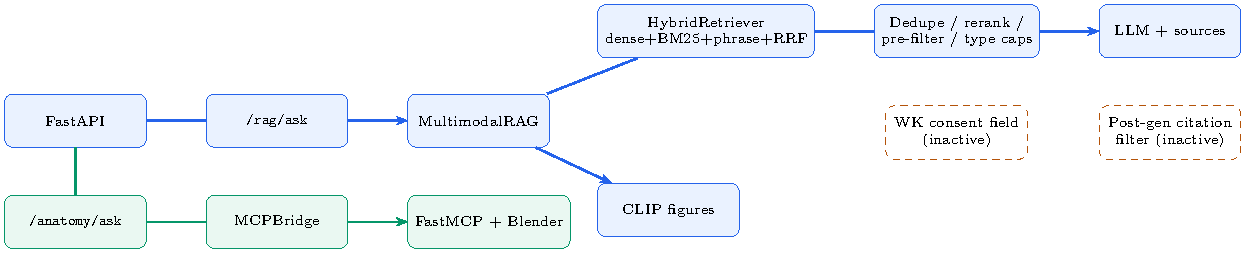
\includegraphics[width=\textwidth,height=0.70\textheight,keepaspectratio]{figures/rendered/final_runtime_architecture.pdf}
  \caption{Code-verified runtime architecture. Active hybrid retrieval stages are shown on the document path. The red block identifies controls that exist in the repository but are not effective on the production \codepath{/rag/ask} request path (notably world-knowledge consent and post-generation citation filtering).}
  \label{fig:final-runtime-architecture}
\end{figure}

The browser interface lives under \codepath{frontend/} and uses Next.js. Its main page contains the document chat, PDF upload controls, and a separate \codepath{AnatomyMcpPanel}. The browser defaults to \codepath{http://127.0.0.1:8000}, whereas the backend image exposes port \texttt{7860}; the frontend is also absent from \codepath{docker-compose.yml}. Deployment therefore requires an explicit API base and port mapping.

FastAPI composition occurs in \codepath{app/main.py}. The file registers ingestion, document-question, experiment, image, storage, visualisation, annotation, legacy Blender, and MCP anatomy routes. It also mounts local figures at \codepath{/outputs}, 3D files at \codepath{/anatomy-exports}, and the Three.js viewer at \codepath{/anatomy-viewer}. CORS origins come from \codepath{ALLOWED_ORIGINS}, with local and hosted defaults.

On the document side, uploads update the text and image indexes before the singleton \codepath{MultimodalRAG} is reloaded. A question then passes through MiniLM--Chroma retrieval, CLIP search, Groq generation, and an optional fixed-asset preview worker. That worker is a legacy HTTP service, not the Z-Anatomy MCP exporter. The 3D route launches \codepath{anatomy_mcp/server.py} as a child process, uses stdio, resolves catalogue entries, invokes Blender after a cache miss, and returns GLB and annotation URLs. This implements MCP's host--client--server separation \parencite{mcp20250618}.

The archive contains two different deployment arrangements. Local MCP operation expects Blender and Z-Anatomy \codepath{Startup.blend} outside the repository. The Compose stack supplies MinIO, the backend, and an older Blender HTTP worker based on \codepath{src/mcp/server.py}; it lacks both the FastMCP Z-Anatomy server and the source blend file. The Compose files therefore document storage and legacy previews rather than a complete containerised MCP deployment.

\section{Repository Structure and Responsibility Mapping}
\label{sec:repository-structure}

\Cref{tab:component-code-map} links each main responsibility to the files that implement it. The final column records what repository inspection established, including components that are not called by the production route.

\begin{table}[htbp]
  \centering
  \small
  \caption{Component-to-code mapping in the frozen repository.}
  \label{tab:component-code-map}
  \begin{tabularx}{\textwidth}{L{0.25\textwidth}L{0.34\textwidth}Y}
    \toprule
    Component & Main location & Verified role \\
    \midrule
    FastAPI composition & \codepath{app/main.py} & Routers, CORS, and static mounts. \\
    Document API & \codepath{app/api/routes/rag.py} & Exposes \codepath{POST /rag/ask}; forwards only \codepath{question}. \\
    Ingestion service & \codepath{app/services/ingestion_service.py} & Saves a PDF, runs text/image ingestion, rebuilds the image index, and reloads RAG. \\
    Text loading & \codepath{src/ingestion/loader.py} & PyMuPDF page loading, page heuristics, and chunking. \\
    Text store & \codepath{src/retrieval/vector_store.py} & Opens the MiniLM-backed Chroma collection under \codepath{processed/chroma}. \\
    Production RAG & \codepath{src/multimodal/multimodal_rag_chain.py} & Hybrid-preferred retrieval, rewrite, dedupe, rerank, pre-filter, type-dependent caps, synthesis, image reranking, grounding metadata. \\
    Hybrid retrieval & \codepath{src/retrieval/hybrid_retriever.py} & BM25, dense, phrase, and RRF; constructed by \codepath{MultimodalRAG}; dense fallback on failure. \\
    Figure pipeline & \codepath{src/ingestion/image_extractor.py}; \codepath{src/multimodal/multimodal_indexer.py} & Embedded-image extraction and complete CLIP-index rebuild. \\
    Storage & \codepath{app/services/object_storage.py} & MinIO/Supabase upload, signed URLs, and diagnostics. \\
    MCP REST layer & \codepath{app/api/routes/anatomy_mcp.py} & Health, search, ask, and export routes. \\
    MCP host/client & \codepath{app/services/anatomy_mcp_chat.py}; \codepath{app/services/anatomy_mcp_client.py} & Fast path, LLM tool loop, stdio session, tool discovery, and tool calls. \\
    MCP server & \codepath{anatomy_mcp/server.py} & Catalogue search, part export, and package export tools. \\
    Catalogue & \codepath{anatomy_mcp/label_index/exportable_catalog.json} & Geometry-probed structure entries. \\
    Blender scripts & \codepath{anatomy_mcp/blender_scripts/} & Z-Anatomy selection, GLB export, annotations, packages, and previews. \\
    Viewer & \codepath{anatomy_mcp/viewer/} & Three.js GLB loading and label display. \\
    \bottomrule
  \end{tabularx}
\end{table}

\section{Next.js Frontend and FastAPI API Layer}
\label{sec:frontend-api}

\subsection{Document Chat and Upload Interface}
\label{subsec:document-ui}

The main page holds the current conversation in browser state. Questions are posted to \codepath{/rag/ask}; PDFs use multipart upload to \codepath{/upload-pdf/}. The renderer can show answer text, source cards, and optional figures. When metadata are present, each source card includes a filename, page, and passage preview.

The frontend also sends \codepath{language} and \codepath{allow_world_knowledge} and displays states for consent and confidence. The frozen backend contract does not support that behaviour: \codepath{AskRequest} contains only \codepath{question}, and the route forwards \codepath{req.question}. Pydantic may ignore the extra fields, but they cannot change the request path. Several response fields expected by the browser are absent from \codepath{AskResponse} as well. For this snapshot, language choice, consent, confidence, and question-type handling are UI intentions rather than active backend controls.

\subsection{MCP Anatomy Interface}
\label{subsec:mcp-ui}

\codepath{AnatomyMcpPanel.js} sends the message and language to \codepath{/anatomy/ask}. Structured success data are handed to \codepath{AnatomyExportPanel}, which creates an iframe only when \codepath{anatomy_export.status == "ok"}. Ordinary errors therefore do not produce an empty viewer.

A compatibility function, \codepath{salvageExportFromAnswer}, searches assistant text for export URLs when structured data are missing. It supports older responses but weakens the verification contract because text-derived URLs may be stale, malformed, or unrelated to a completed tool call. Evaluation should either disable this path or record salvage-only cases separately.

\subsection{FastAPI Composition and Static Serving}
\label{subsec:fastapi-composition}

Route files parse requests and delegate to service modules. RAG uses \codepath{rag_service.py}, ingestion uses \codepath{ingestion_service.py}, storage uses \codepath{object_storage.py}, and anatomy requests pass to the MCP host. Generated files stay outside the frontend project; the backend exposes the relevant directories through static mounts and returns loadable URLs.

\section{PDF Ingestion, Cleaning, Chunking, and Metadata}
\label{sec:pdf-ingestion}

\codepath{upload_pdf} checks the file extension, writes the PDF to the raw-data directory, and performs a storage preflight. Text ingestion, image extraction, multimodal indexing, and \codepath{reload_rag} then run in sequence. The API response records status and elapsed time for each stage, so a partial failure remains visible.

The text loader scans every PDF in the raw directory with \codepath{PyMuPDFLoader}. It applies three inexpensive heuristics for likely index, contents, and glossary pages: an early ``index'' token, dotted chapter headings, and short comma-dense pages. These checks remove obvious noise but may also discard valid anatomy material. They are project-specific heuristics, not general PDF-cleaning guarantees.

Retained pages are divided by \codepath{RecursiveCharacterTextSplitter} into 800-character chunks with 150 characters of overlap. Fragments below 200 characters and dotted contents-like text are removed. Source and page metadata survive the split. The system embeds text with \codepath{sentence-transformers/all-MiniLM-L6-v2} \parencite{reimers2019,minilmModelCard} and appends records to collection \codepath{multimodal_rag} under \codepath{processed/chroma}.

Text indexing is append-oriented: the collection is not cleared, and stable identifiers are not derived from file and chunk hashes. Re-running ingestion over the same directory can create duplicate vectors. Retrieval-time filtering reduces repeated source cards without cleaning the store. A reproducible run should rebuild the collection from a clean, versioned corpus manifest.

Image ingestion behaves differently. Embedded raster images are enumerated, written locally, and stored with source, page, context, dimensions, and an object key. The service attempts upload to the configured object store, after which the multimodal index is cleared and rebuilt from valid metadata. Text and image indexes therefore have different update semantics.

\section{Text Retrieval: Hybrid-Preferred Production Route}
\label{sec:text-retrieval}

\subsection{Active Production Retrieval}
\label{subsec:active-text-retrieval}

\Cref{fig:rag-runtime-sequence} shows the active document path. \codepath{MultimodalRAG} constructs \codepath{HybridRetriever} once at initialisation and caches the BM25 index on disk. For each question it classifies the type, rewrites query variants, and requests hybrid candidates (dense, BM25, and phrase) with Reciprocal Rank Fusion defaults of 0.5, 0.4, and 0.1 and RRF constant 60 \parencite{karpukhin2020,robertson2009,cormack2009,reimers2019}. Candidate pools use up to 40 documents per query variant and a fused final pool of 32 before deduplication and reranking. If hybrid construction or search fails, the chain falls back to dense Chroma \codepath{similarity\_search}.

\begin{figure}[htbp]
  \centering
  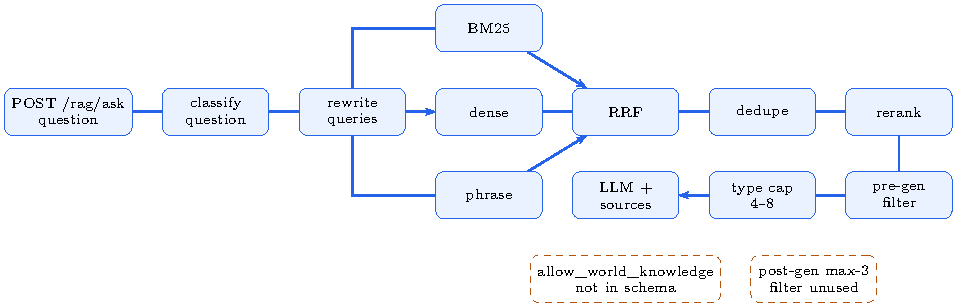
\includegraphics[width=\textwidth,height=0.68\textheight,keepaspectratio]{figures/rendered/rag_runtime_sequence.pdf}
  \caption{Production document request sequence after hybrid connection. Dashed orange notes identify repository controls that are not effective on this route (world-knowledge consent field; post-generation citation filter).}
  \label{fig:rag-runtime-sequence}
\end{figure}

Two keys remove duplicate passages. The first is a SHA-256 fingerprint of roughly the first 220 normalised characters; the second joins a normalised PDF stem with the page number. Surviving passages are support-score reranked and passed through a pre-generation citation filter. Final context size is selected by question type through \codepath{max_passages_for_type}, typically four to eight unique passages rather than the earlier hard three-passage design. The same records form both the model context and the source-card list.

\subsection{Hybrid Retriever Construction and Dense Fallback}
\label{subsec:hybrid-connected}

\codepath{HybridRetriever} combines dense search, BM25, phrase matching, and weighted RRF. BM25 contributes lexical evidence \parencite{robertson2009}, dense retrieval contributes semantic evidence \parencite{karpukhin2020}, and RRF combines ranking positions rather than incompatible raw scores \parencite{cormack2009}. The class is constructed inside \codepath{MultimodalRAG} initialisation and called from \codepath{\_retrieve\_text\_corpus} on the \codepath{/rag/ask} path. Dense-only search is retained as fallback behaviour, not as the primary evaluated mode. No selectable dense/BM25/hybrid evaluation switch existed at the time of the July run, and no matched dense-only versus hybrid ablation was completed.

\section{Query Processing, Reranking, Deduplication, and Evidence Grading}
\label{sec:query-evidence}

Question classification, typo correction, query rewriting, support-score reranking, and pre-generation citation filtering are imported by the production chain under \codepath{src/rag/} and used on \codepath{/rag/ask}. Evidence grading, post-generation citation filtering with a hard three-source limit, and answer-verification modules also exist and are covered by unit tests, but they are not the effective controls on the evaluated ask path. Images follow a separate CLIP reranking path. A thesis experiment endpoint can create baseline and stricter answers from the same retrieval bundle, but it neither replaces the main endpoint nor changes the hybrid-preferred default. These boundaries determine what can be described as verified runtime behaviour.

\section{Answer Synthesis, Sources, Abstention, and Grounding Metadata}
\label{sec:answer-synthesis}

The language-model factory creates \codepath{ChatGroq} with \codepath{llama-3.1-8b-instant} at temperature zero. The production prompt asks the model to use context and prefer supported facts, but it does not require claim identifiers, run a post-generation entailment check, or enforce refusal.

Available text passages are concatenated into the prompt. If neither text nor a multimodal excerpt is present, the prompt allows a general-knowledge response and asks for a disclaimer. This fallback is independent of the unused frontend consent field. Returned \codepath{sources} are retrieval records rather than verified sentence-level citations.

The response includes \codepath{grounding.primary_basis}, \codepath{provenance_explanation}, and \codepath{evaluation_note}. These fields record whether retrieved material reached the prompt; they are processing metadata, not measures of factual or anatomical confidence. The July run is consequently analysed as document-assisted generation rather than a strictly enforced document-only system.

\section{CLIP Image Extraction, Indexing, Retrieval, and Late Fusion}
\label{sec:clip-pipeline}

Images are indexed separately under \codepath{processed/multimodal_chroma} with \codepath{clip-ViT-B-32}. CLIP encodes text and images in a compatible space, enabling text-to-image search \parencite{radford2021}. Each record stores an embedding together with caption, local path, object key, source, and page metadata.

At query time, \codepath{MultimodalRetriever.retrieve} encodes the question, requests up to 20 records, converts distance to \codepath{1-distance}, and initially retains scores above 0.10. If no record survives, the method falls back to the leading candidates. This guarantees material for reranking but can also carry weak images further through the pipeline.

Image reranking combines caption similarity from the text embedding model with CLIP image similarity when a local file is available. The score weights CLIP at 0.25 and caption similarity at 0.75. Local candidates use a threshold of 0.18; remote-only records use 0.10. Up to five records reach URL construction before duplicate filtering reduces the response to three images.

Text and image scores are never merged. The answer, source objects, and figure URLs meet only in the API response. This late-fusion design keeps both modalities inspectable and prevents the presence of an image from being treated as proof that the text is correct.

\section{Local, MinIO, and Supabase Storage}
\label{sec:storage}

\codepath{object_storage.py} selects MinIO or Supabase through environment variables. MinIO is used in the local Compose stack, while Supabase requires a project URL and service-role key. The service supports bucket diagnostics, byte uploads, and signed GET URLs through \codepath{/debug/storage}.

For each figure, the RAG chain first requests a signed object URL. If signing fails and a local copy exists, the file is placed in the public output directory and served through \codepath{/outputs}. The fallback is convenient in development but ties URL behaviour to the environment and backend process lifetime.

MCP exports use another path. They remain under \codepath{anatomy_mcp/exports} and are published through a static mount rather than the object-storage layer. Shared storage or an external artefact service would be required for ephemeral or multi-replica deployment.

\section{MCP Host and MCPBridge Client}
\label{sec:mcp-host-client}

\codepath{anatomy_mcp_chat.py} supports two orchestration paths. A concise structure-like request enters a deterministic fast path: the host calls \codepath{search_anatomy_catalog}, selects the best unique exportable label, and invokes an export tool. More complex or unresolved wording enters an LM Studio tool loop limited to six rounds. Tool definitions are discovered from the live MCP session, and every proposed call is executed through the bridge before its structured result is added to the conversation.

The protocol boundary is implemented by \codepath{MCPBridge}. It creates \codepath{StdioServerParameters} for the current Python executable and \codepath{anatomy_mcp/server.py}, starts \codepath{stdio_client}, initialises a \codepath{ClientSession}, lists tools, and calls them. Structured content is preferred; text parsing is only a fallback. Export functions are therefore reached through an actual MCP client/server session rather than direct imports.

\begin{figure}[htbp]
  \centering
  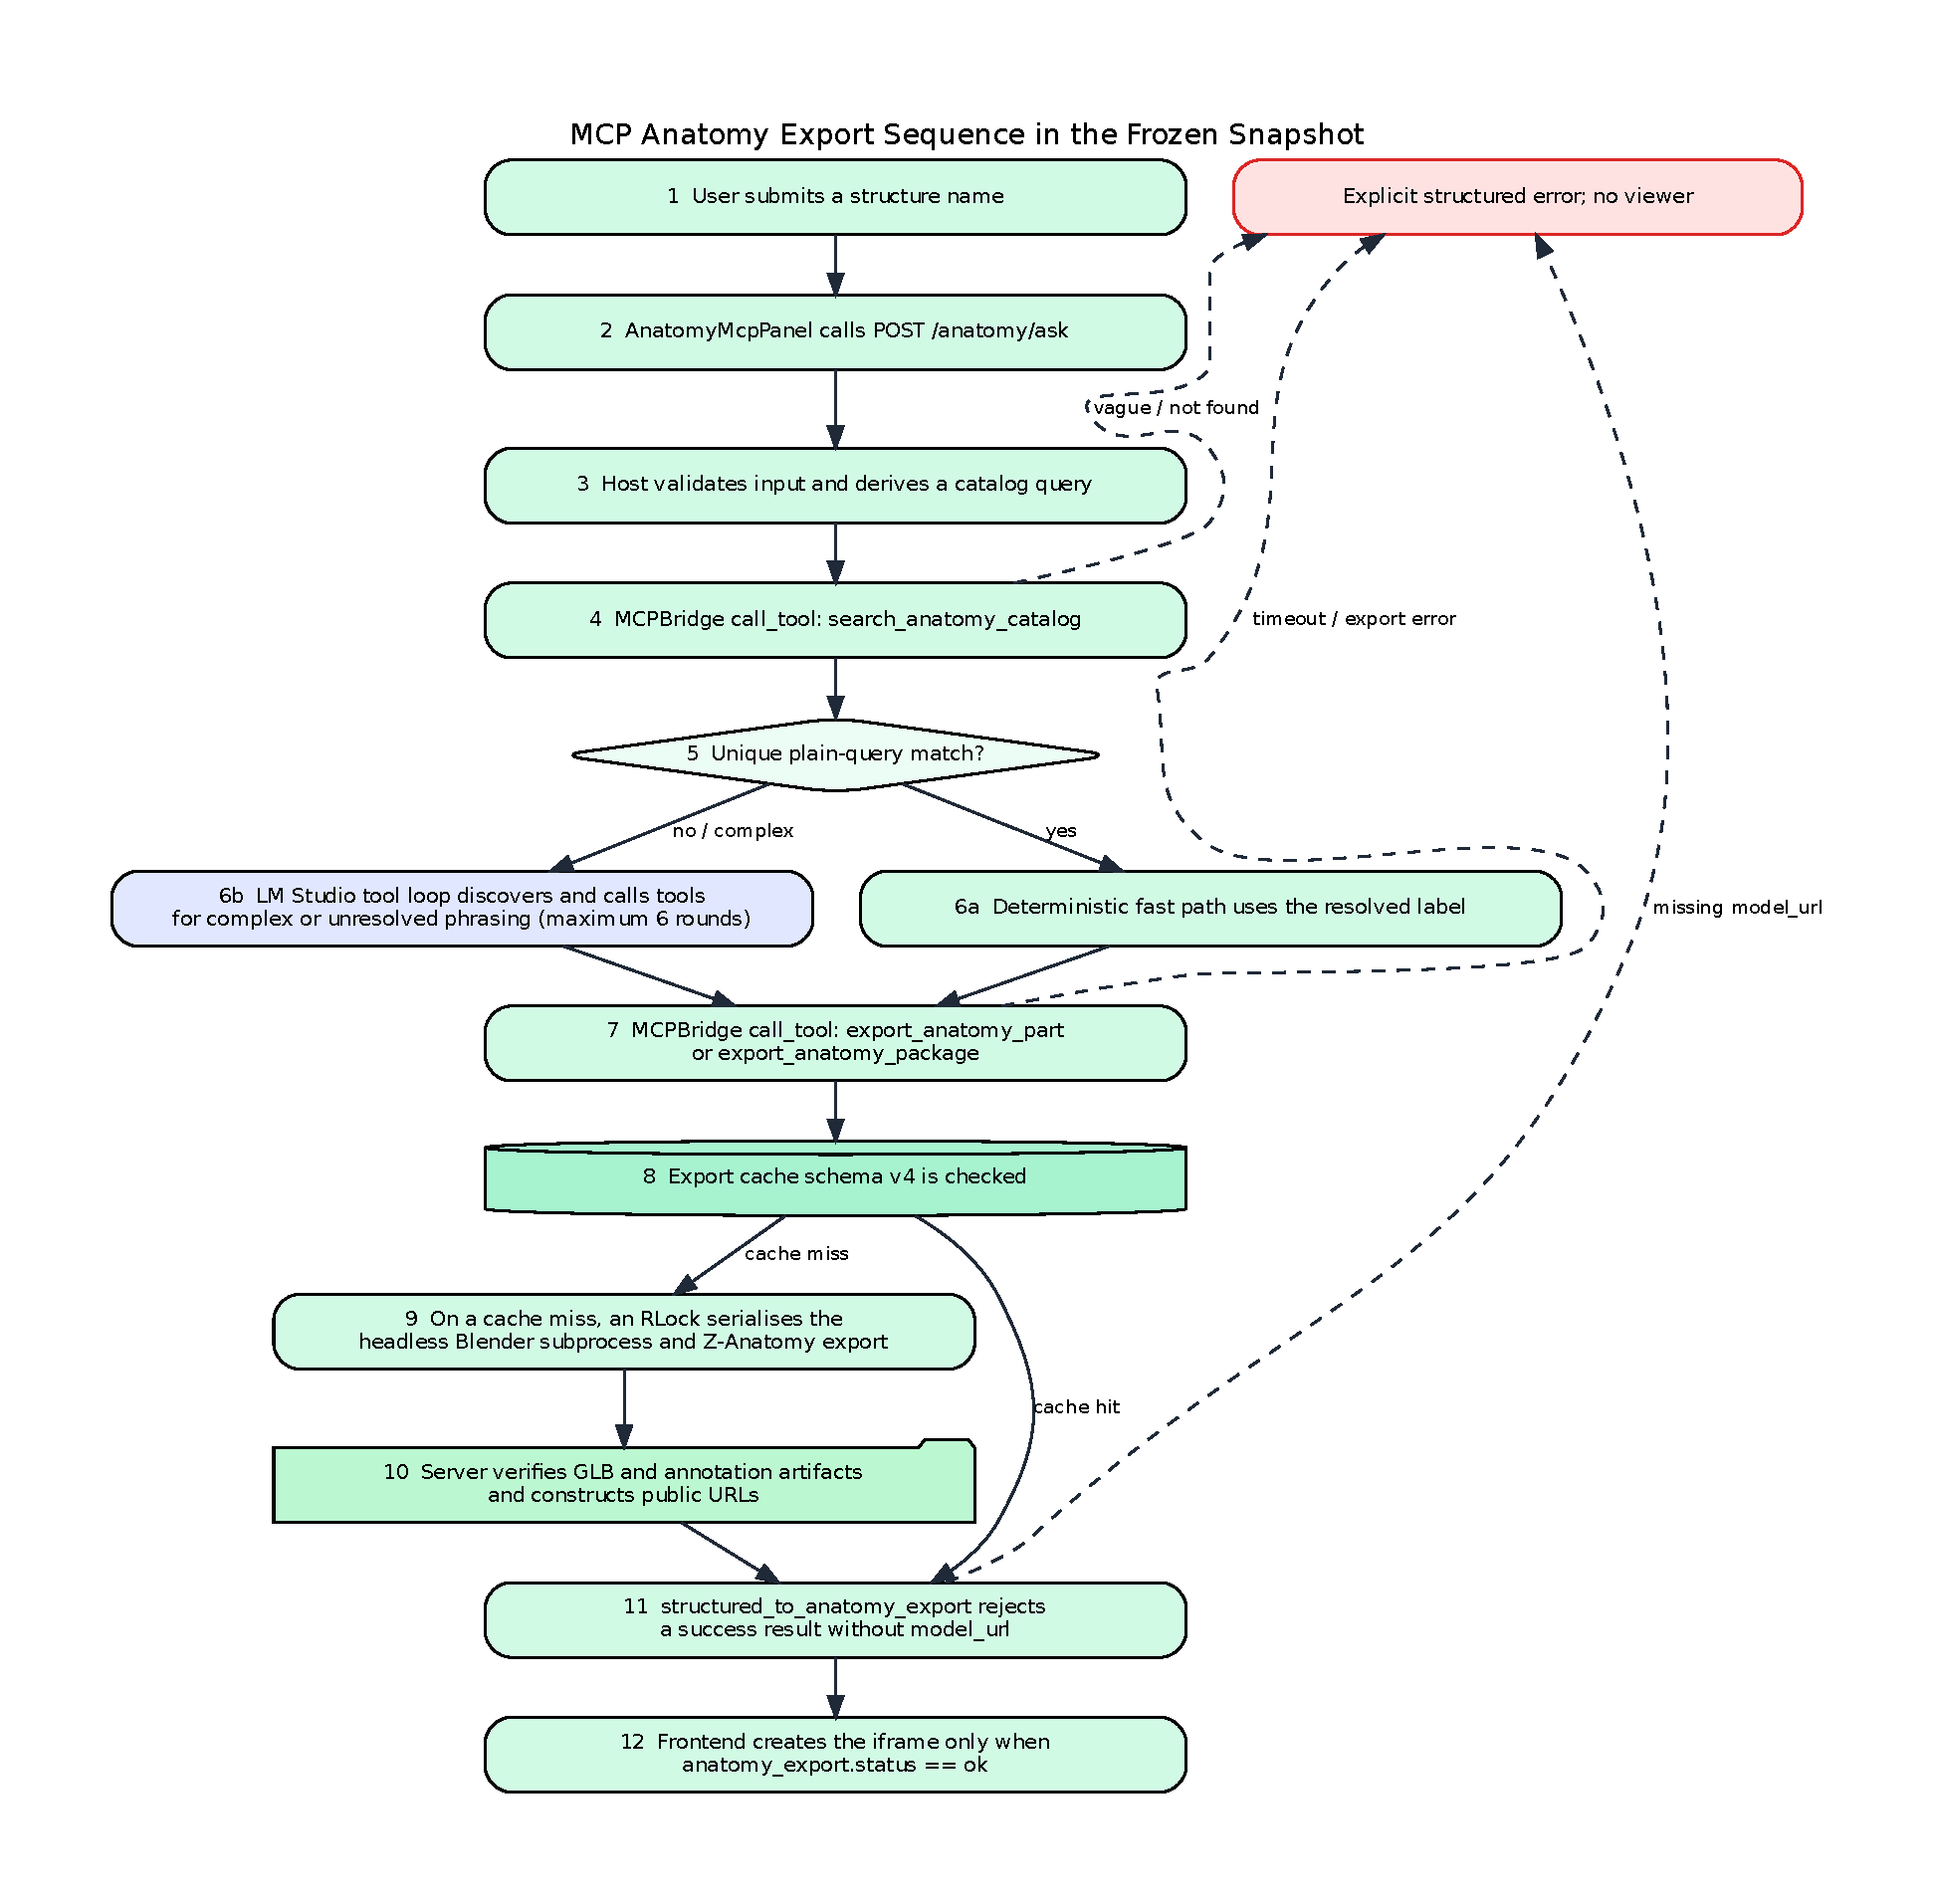
\includegraphics[width=\textwidth,height=0.68\textheight,keepaspectratio]{figures/rendered/mcp_runtime_sequence.pdf}
  \caption{MCP anatomy export sequence, including fast path, LLM tool loop, cache, Blender export, and explicit failure branches.}
  \label{fig:mcp-runtime-sequence}
\end{figure}

The host records \codepath{mcp_tools_used} and \codepath{mcp_tool_steps}. \codepath{structured_to_anatomy_export} creates a successful export object only if the tool result contains \codepath{model_url}. When configured, URL rewriting replaces development hosts with \codepath{PUBLIC_API_BASE}.

\section{FastMCP Server and Tool Schemas}
\label{sec:fastmcp-server}

The child process creates \codepath{FastMCP("Anatomy Blender MCP", json_response=True)} and exposes the tools in \cref{tab:mcp-tools}. Validation occurs before catalogue access or subprocess execution. Queries are limited to 80 characters and a conservative character set; Blender scripts and output paths are selected internally rather than supplied by the user.

\begin{table}[htbp]
  \centering
  \small
  \caption{FastMCP tools and structured responsibilities.}
  \label{tab:mcp-tools}
  \begin{tabularx}{\textwidth}{L{0.25\textwidth}L{0.28\textwidth}Y}
    \toprule
    Tool & Main input & Responsibility \\
    \midrule
    \codepath{search_anatomy_catalog} & Query and result limit & Validates and ranks exportable labels; returns laterality, match type, counts, suggestions, and catalogue metadata. \\
    \codepath{export_anatomy_part} & Part query, preview flag, optional region hint & Resolves one structure, serves a cache hit or runs Blender, verifies GLB/annotations, and returns public URLs. \\
    \codepath{export_anatomy_package} & Part query and package options & Exports large structures with a main GLB, annotations, manifest, optional materials, per-object files, preview, and timing metadata. \\
    \bottomrule
  \end{tabularx}
\end{table}

Explicit error codes distinguish vague, missing, ambiguous, configuration, timeout, subprocess, and artefact failures. The UI can handle these categories deterministically, and evaluation can score them separately. Arbitrary blend-file paths and Python programs are excluded from the schema.

\section{Geometry Catalogue and Structure Resolution}
\label{sec:catalog-resolution}

The bundled \codepath{exportable_catalog.json} uses schema version 1 and contains 6,075 entries: 555 collections and 5,520 objects. Its archive SHA-256 is \nolinkurl{a18357fb83bda6a1b9b3f329ead4be50dc2c26196200fe6358e73b51174d6350}. The recorded source path ends in \codepath{Startup.blend}, although the blend file is external. \codepath{build_exportable_catalog.py} retained entries with detected geometry. A complete evidence package still needs the exact Z-Anatomy release, licence, and blend-file hash \parencite{zanatomy}.

\codepath{query_validation.py} normalises natural-language input. The resolver checks exact and known aliases before token ranking and laterality rules. A phrase such as ``left femur'' can therefore resolve to \codepath{Femur.l} when the result is unique. Ambiguous cases return candidates rather than silently selecting the first match.

If the exportable catalogue is missing, the resolver can fall back to \codepath{z_anatomy_index.json} and sets \codepath{resolver_source=raw_index}. This preserves older behaviour but weakens the geometry-proven assumption. Evaluation records should therefore include the resolver source.

\section{Blender Export, GLB, Annotations, and Three.js}
\label{sec:blender-viewer}

After resolution, the server selects a part or package exporter, creates unique output paths, and launches Blender in background factory-startup mode. The command includes the external blend path, exporter script, canonical label, and resolved objects or collections. Default timeouts are 300 seconds for a part and 900 seconds for a package.

The subprocess runs within a process-wide re-entrant lock. Standard input is disconnected from the MCP transport, and standard error is merged with standard output. The server parses the final JSON object from the exporter, checks the return code and \codepath{ok} field, and verifies the GLB and annotation files. Requested previews are checked as well. Public URLs are built only after these conditions pass.

Blender's glTF pipeline produces the exported model \parencite{blenderGltf}. GLB contains browser-compatible geometry and scene data; annotations remain in a separate JSON file. The Three.js viewer uses \codepath{GLTFLoader} and \codepath{OrbitControls}, frames the model from its bounds, adds lighting, and places labels at annotation anchors. A successful protocol exchange confirms the file path, not the anatomical correctness of the resolved geometry, transforms, or annotations.

\section{Locking, Caching, Health Checks, and Safe Errors}
\label{sec:reliability}

\codepath{\_BLENDER_EXPORT_LOCK = threading.RLock()} serialises Blender calls inside one MCP server process. That fits the target single-machine Windows setup but cannot coordinate several processes or machines. Scaling would require an inter-process or distributed mechanism.

Cache schema \codepath{v4} builds part keys from schema version, canonical label, match type, and preview mode; package keys also include package options. A hit is accepted only when GLB and annotation files exist and the annotation JSON contains a record. Tool results expose \codepath{cache_hit} for later comparison. Because the key omits hashes of the blend file, catalogue, and exporter scripts, those changes require a schema update or cache deletion.

\codepath{/anatomy/health} checks Blender, the source blend, indexes, the MCP import, and the stdio bridge. Catalogue presence is reported but not required by the current \codepath{ready} expression, so the endpoint may claim readiness even when search would fail. A stronger probe would require the exportable catalogue and a successful tool-list or search call.

The host rejects structured success without \codepath{model_url}, and the frontend opens the viewer only for \codepath{status == ok}. Tool errors stay explicit; text salvage is the weaker exception. Unit tests cover query validation, left-femur resolution, URL normalisation, mocked tool loops, and rejection of unverified export prose. They do not run the external Blender/Z-Anatomy stack. API-test collection during the audit also failed because \codepath{openai} was absent from the installed environment, exposing a packaging gap.

\section{API Contract Summary}
\label{sec:api-contracts}

\begin{table}[htbp]
  \centering
  \small
  \caption{Principal HTTP contracts in the frozen FastAPI application.}
  \label{tab:api-contracts}
  \begin{tabularx}{\textwidth}{L{0.23\textwidth}L{0.09\textwidth}L{0.27\textwidth}Y}
    \toprule
    Endpoint & Method & Request & Principal response \\
    \midrule
    \codepath{/upload-pdf/} & POST & Multipart \codepath{file} & Stage status, text ingestion, image extraction, and elapsed time. \\
    \codepath{/rag/ask} & POST & \codepath{question} & Answer, sources, images, grounding metadata, and optional legacy render fields. \\
    \codepath{/rag/experiment/ask} & POST & Question and log flag & Baseline/strict answers, sources, judge output, and debug fields. \\
    \codepath{/anatomy/health} & GET & None & Configuration and stdio readiness checks. \\
    \codepath{/anatomy/search} & GET & Query \codepath{q}, optional limit & Catalogue result, suggestions, or structured error. \\
    \codepath{/anatomy/ask} & POST & Message and language & Answer, \codepath{anatomy_export}, tool audit trail, mode, and error. \\
    \codepath{/anatomy/export} & POST & Part query and export options & Structured export result or error. \\
    \codepath{/debug/storage} & GET & None & Provider, bucket checks, and sample keys. \\
    \codepath{/images/all} & GET & None & Local image URL list. \\
    \codepath{/blender/generate-brain-3d} & POST & Legacy generation request & Asset/preview URLs or error. \\
    \bottomrule
  \end{tabularx}
\end{table}

The schemas preserve the mode boundary. \codepath{AskResponse} is document-oriented, whereas \codepath{AnatomyAskResult} carries a structured artefact and tool trace. Most frontend/backend drift occurs in the document contract.

\section{Configuration and Reproducibility}
\label{sec:configuration-reproducibility}

Requirements files, \codepath{package-lock.json}, Docker images, model identifiers, and repository commits provide partial version evidence. \Cref{tab:environment-versions} separates the audit HEAD, the hybrid-connection commit, the earlier dense-only inspection snapshot, and declared dependency values from information that depends on the final machine.

\small
\setlength{\tabcolsep}{3pt}
\begin{longtable}{L{0.23\textwidth}L{0.39\textwidth}L{0.29\textwidth}}
  \caption{Environment and version record for the audited implementation timeline.}
  \label{tab:environment-versions}\\
  \toprule
  Item & Repository-declared value & Final evidence status \\
  \midrule
  \endfirsthead
  \caption[]{Environment and version record (continued).}\\
  \toprule
  Item & Repository-declared value & Final evidence status \\
  \midrule
  \endhead
  \midrule
  \multicolumn{3}{r}{Continued on next page}\\
  \endfoot
  \bottomrule
  \endlastfoot
  Audit snapshot & \nolinkurl{d3a544d0b2202b1e068b648968a2ae17f871bfa8} & Thesis audit HEAD; not a claim that every dependency was frozen with P1. \\
  Hybrid-connection commit & \nolinkurl{5089fcc0182f86c71558ccce21b75ebcb18b06f4} (12 July 2026) & \codepath{HybridRetriever} wired into \codepath{MultimodalRAG}/\codepath{/rag/ask}; preferred P1 route. \\
  Historical dense-only snapshot & \nolinkurl{cb041d52787f469bbbe0434e9fc7690edc122afa} (27 June 2026) & Earlier inspection baseline only; not the final or July-evaluated implementation. \\
  Backend base & Python \codepath{3.11-slim} & Runtime patch version required. \\
  Next.js / React & Next.js \codepath{16.2.4}; React/ReactDOM \codepath{19.2.5} & Lock-file verified; Node.js version required. \\
  Embedding libraries & \codepath{sentence-transformers==2.7.0}; \codepath{transformers==4.41.2} & Declared; installed freeze required. \\
  Text model & \codepath{sentence-transformers/all-MiniLM-L6-v2} & Model revision/cache hash required. \\
  CLIP model & \codepath{clip-ViT-B-32} & Model revision/cache hash required. \\
  Torch / NumPy & \codepath{torch==2.2.2}; \codepath{numpy==1.26.4} & Declared. \\
  Chroma & \codepath{chromadb>=1.5.0}; LangChain Chroma unpinned & Exact installed versions required. \\
  RAG model & Groq \codepath{llama-3.1-8b-instant} & Provider revision/date required. \\
  MCP endpoint & \codepath{LLM_API_BASE}; default \codepath{http://127.0.0.1:1234/v1} & Environment-configurable. \\
  MCP model & \codepath{settings.llm_model = llama-3.1-8b-instant} & Runtime identifier must be verified. \\
  MCP SDK & \codepath{mcp[cli]>=1.27.1} in a separate requirements file & Installed version required. \\
  Blender & Local default references 5.1; legacy image installs 4.0.2 & Actual MCP binary/version required. \\
  Z-Anatomy & External \codepath{Startup.blend} & External asset; exact release and source-file hash were not archived with the evaluation \\
  Catalogue & Schema 1; 6,075 entries; SHA-256 \nolinkurl{a18357fb83bda6a1b9b3f329ead4be50dc2c26196200fe6358e73b51174d6350} & Archive verified. \\
  Storage & MinIO or Supabase selected by environment & Provider, bucket policy, and URL expiry required. \\
  Hardware / OS & Not recorded & Hardware details were not archived; evaluation date was 12 July 2026 \\
\end{longtable}
\normalsize

The declared environment has three dependency gaps. \codepath{anatomy_mcp_chat.py} imports \codepath{openai.AsyncOpenAI}, but the root requirements omit \codepath{openai}. \codepath{HybridRetriever} depends on undeclared \codepath{rank_bm25}. The MCP SDK appears only in \codepath{anatomy_mcp/requirements.txt}, while the backend Dockerfile installs the root requirements. Additional installation is therefore required before the backend image can be assumed to run the MCP path.

Model configuration drifts as well. \codepath{.env.example} documents \codepath{LLM_MODEL=qwen2.5-7b-instruct-1m}, while \codepath{Settings.llm_model} is a constant shared by Groq synthesis and the LM Studio tool loop. Separate RAG and MCP variables would make the resolved runtime easier to record and test.

A reproducible release still requires corpus hashes, a deterministic index build, prompt versions, object-storage settings, Blender and Z-Anatomy hashes, the catalogue hash, hardware, operating system, and evaluation date. The repository supports a detailed source-level architecture account, but the missing runtime record prevents a claim of fully reproducible deployment.

\section{Chapter Summary}
\label{sec:implementation-summary}

The archive contains a substantial implementation: PDF ingestion, MiniLM--Chroma and BM25 hybrid retrieval, CLIP figure search, duplicate filtering, type-dependent context selection, local or cloud generation, object-storage URLs, an MCP stdio boundary, catalogue resolution, locked and cached Blender export, artefact checks, and a guarded Three.js viewer. The MCP route is close to the documented architecture. The document route is hybrid-preferred after \texttt{5089fcc}, while world-knowledge consent enforcement and post-generation citation verification remain incomplete on \codepath{/rag/ask}. The evaluation and conclusions therefore follow the verified active route rather than every module present in the repository.

\chapter{Evaluation Methodology}
\label{chap:evaluation}

The project did not produce one neat, final experiment. Its evidence accumulated while the system was still changing: a formative workbook captured early weaknesses, a larger English run recorded the broadest set of outcomes, a small German set exposed several concrete failures, and an earlier model comparison used conditions that were not fully aligned. Rather than combine these records into a single headline score, I separate them according to the question each one can reasonably answer. The same rule is applied to work that was planned but not completed. A dense-versus-hybrid ablation, an expert figure-relevance study, and the MCP runtime comparison are described as missing experiments, not reconstructed after the fact.

\section{Evaluation Design and Units of Analysis}
\label{sec:evaluation-design}

RAG and MCP were treated as different technical objects because their failure chains are different. A document request may fail before generation, retrieve the wrong passage, use evidence poorly, or attach an unsuitable source or image. A 3D request must first resolve a structure, then call a tool, create files, publish URLs, and load the model. A single combined score would conceal which of these stages failed.

For the RAG path, I kept three denominators visible. Request reliability covers every submitted question, including timeouts and HTTP errors. Retrieval analysis is possible only when the response contains a usable passage list. Answer and boundary behaviour is then examined from the retained classifications and selected manual cases. This choice matters for the four failed English requests: they count against operational reliability, but they cannot contribute to a ranking metric because no complete result was returned.

\section{Evaluation Runs and Evidence Hierarchy}
\label{sec:evaluation-runs}

Five records were available. Their roles are shown in \cref{tab:evaluation-run-register}; only P1 was used as the main quantitative run.

\begin{table}[htbp]
  \centering
  \caption{Evaluation runs used in this thesis.}
  \label{tab:evaluation-run-register}
  \small
  \begin{tabularx}{\textwidth}{L{0.13\textwidth}L{0.18\textwidth}L{0.19\textwidth}Y}
    \toprule
    Run & Dataset & Role in thesis & Evidential status \\
    \midrule
    F1 & 15 English questions & Formative manual rubric & Used to identify quotation, typo, citation, and boundary weaknesses; not a frozen final-system result. \\
    P1 & 55 English questions, 12 July 2026 & Primary RAG run & Main quantitative evidence; 51 usable responses and four infrastructure failures. Configuration was only partially archived. \\
    D1 & Nine German questions & Diagnostic anatomy and language check & Seven substantive responses, one HTTP 500, and one timeout; used for failure analysis rather than aggregate performance. \\
    M1 & Earlier Qwen, Gemma, and document-grounded comparison & Exploratory model comparison & Conditions were not sufficiently controlled for causal model claims. \\
    MCP-P & Planned MCP worksheet & Design protocol only & No completed result rows; used to define future verification requirements, not as empirical evidence. \\
    \bottomrule
  \end{tabularx}
\end{table}

P1 was chosen because it is the largest record and preserves raw responses, outcome labels, and automatic retrieval summaries. Even so, it is not a fully frozen experiment. The evaluated commit, corpus manifest, prompt revision, complete dependency state, model quantisation, hardware, and route trace were not archived together. The analysis can reconstruct the scoring procedure, but an exact rerun would require information that was not preserved.

The remaining records are used more narrowly. F1 explains why quotation handling, typo recovery, citation filtering, and boundary control became design concerns. D1 provides concrete language, infrastructure, and anatomy failure cases. M1 suggests that the model and the surrounding pipeline both influenced the answers, but the conditions are too different for a causal model ranking. I did not pool any of these datasets with P1.

\section{Primary English RAG Dataset}
\label{sec:rag-dataset}

P1 contains 55 questions: 15 direct factual items, 10 complex or multi-part items, 10 figure-related items, five quotation requests, 10 boundary or off-topic questions, and five robustness variants. The purpose was coverage of known risks, not estimation of performance across anatomy in general.

Each category stresses a different part of the application. Direct and complex questions ask whether the corpus contains usable textual support. Figure questions exercise the image-return path. Quotation requests require exact wording rather than a plausible paraphrase. Boundary cases include unsupported topics, false premises, and off-topic requests. The robustness set changes wording or introduces typographical variation.

Boundary cases could not be scored through a single refusal rule. A false premise may call for correction, whereas an unsupported document question may require an explicit limitation. I retained the workbook label for traceability, but I also inspected the raw response when the expected behaviour was ambiguous. That decision is important because one of the preliminary labels did not fit the recorded answer cleanly.

\section{Execution Procedure and Recorded Configuration}
\label{sec:rag-procedure}

Each P1 question was submitted to \codepath{POST /rag/ask}. The run register identifies \codepath{qwen3.5-9b-deepseek-v4-flash} in LM Studio through its local OpenAI-compatible endpoint. It also records \codepath{allow_world_knowledge=false}. Later repository inspection showed that the production \codepath{AskRequest} schema accepted only \codepath{question}; the additional field therefore could not influence the active backend route. I kept that mismatch in the analysis because it explains part of the observed world-knowledge leakage.

\subsection{Primary P1 configuration}
\label{subsec:p1-configuration}

P1 is defined as a hybrid-preferred production run of \codepath{/rag/ask} evaluated after commit \texttt{5089fcc} (12~July~2026), when \codepath{HybridRetriever} was connected to \codepath{MultimodalRAG}. Dense similarity search remained available only as a fallback if hybrid construction or search failed. No selectable dense/BM25/hybrid evaluation mode existed, the exact per-request retrieval mode was not recorded in \codepath{eval/rag_eval_55_results.json}, and no matched dense-only versus hybrid ablation was completed. Hybrid superiority is therefore outside the scope of P1.

An earlier dense-only snapshot (\texttt{cb041d5}, 27~June~2026) used up to 24 candidates and a hard three-passage cap. That design is retained as historical context in \cref{chap:evolution}. The July responses instead show a mean of 5.16 sources and a distribution consistent with question-type-dependent caps of approximately four to eight. I use the saved metadata as the empirical record rather than trimming responses to match the earlier design.

\section{Request Reliability and Outcome Classification}
\label{sec:reliability-method}

Request completion was calculated as
\[
\operatorname{CompletionRate}=\frac{\text{requests with a usable response}}{\text{administered requests}}.
\]
Timeouts and HTTP failures remain in the denominator because they affect whether the prototype can be used at all. For completed requests, the workbook classified the main basis of the answer as corpus-derived, world knowledge, or abstention. These labels are judgements about the retained outputs. They are not claim-level demonstrations of faithfulness. Source-object presence was recorded separately for the same reason: an attached passage can be topically related without supporting the answer.

\section{Automatic Retrieval-Proxy Analysis}
\label{sec:retrieval-proxy-method}

No expert-labelled passage set was available. The retained analysis therefore used an automatic proxy. For each non-boundary question, the question and expected key points were combined into a reference representation, encoded with \codepath{all-MiniLM-L6-v2}, and compared with the returned passages. A cosine similarity of at least 0.38 marked a passage as proxy-relevant. The threshold comes from \codepath{scripts/retrieval_metrics.py}; I found no calibration set or sensitivity analysis that would justify it as a domain-specific cut-off.

For question $q$, let $D_q^{(k)}$ denote the first $k$ returned passages and let $R_q$ denote the passages marked relevant by the proxy. The reported automatic measures are:
\begin{align*}
\operatorname{Precision@}k&=\frac{|D_q^{(k)}\cap R_q|}{k},
\qquad
\operatorname{Recall@}k=\frac{|D_q^{(k)}\cap R_q|}{|R_q|},
\end{align*}
together with Precision@1, Precision@3, Recall@1, Recall@3, MRR (reciprocal rank of the first proxy-relevant passage; zero if none), nDCG@3 \parencite{jarvelin2002}, and source overlap between proxy-relevant keys in the top-3 and all returned proxy-relevant passages. The principal macro-average covers 43 non-boundary questions. A second summary includes all 51 completed responses to show how boundary cases change the aggregate. Request-completion rate uses all 55 administered questions in the denominator; infrastructure failures remain excluded from retrieval macros but retained in reliability reporting.

These measures describe rank order under one consistent automatic embedding-similarity rule. Their limitations are substantial. A MiniLM-family representation influenced both the retrieval environment and the evaluation, so the two stages may favour similar semantic patterns. The binary threshold also turns a continuous similarity score into a relevance judgement without expert calibration. I therefore report the proxy values as early ranking evidence, not as anatomy-expert relevance, faithfulness, or answer-correctness scores.

\section{Answer, Grounding, Citation, and Anatomy Review}
\label{sec:answer-review-method}

P1 did not preserve a complete claim-level annotation. As a result, it cannot support aggregate percentages for correctness, completeness, faithfulness, hallucination, citation correctness, citation completeness, or exact-quotation accuracy. I used the evidence that was actually available:

\begin{enumerate}
  \item the corpus/world-knowledge/abstention classification;
  \item the presence of retrieved passages and source objects;
  \item manual inspection of selected boundary and quotation cases; and
  \item anatomy-focused inspection of the German diagnostic responses.
\end{enumerate}

This material is sufficient to identify specific errors and inconsistencies, but not to estimate overall anatomical accuracy. I also kept source presence separate from citation quality. A stronger citation study would segment each answer into substantive claims, check whether the attached passage supports each claim, verify that evidence-requiring claims are cited, and compare any quoted wording with the source \parencite{gao2023alce}.

\section{Multimodal Figure Assessment}
\label{sec:image-evaluation-method}

Only one figure measure was complete: whether a figure-related request returned at least one image object. Ten questions were available. The saved records do not include expert Top-1 relevance, Precision@$k$, image--answer consistency, duplicate rate, broken-link rate, or source-page verification. Observations of irrelevant images from development are therefore reported qualitatively rather than converted into a percentage.

This measure tests whether the image path was integrated into the response. It says little about whether the image was useful. CLIP offers a practical route from text to image retrieval, but a general-domain representation can miss fine anatomical distinctions and small labels \parencite{radford2021,wang2022medclip}. Availability and relevance are consequently reported as separate outcomes.

\section{German Diagnostic Set and Formative Comparisons}
\label{sec:diagnostic-method}

The German diagnostic set contains nine requests. Seven produced substantive responses, one returned HTTP 500, and one timed out. I reviewed the retained outputs for boundary behaviour, terminology, and clear anatomy errors. One extraocular-muscle response assigned the oblique muscles to the wrong cranial nerves; this was checked against an external anatomy source \parencite{purves2001extraocular}. With only nine questions and limited annotation, the set is used to document failure modes rather than to estimate accuracy.

F1 and M1 serve a similar historical purpose. F1 recorded 10 passes, two passes with caveats, one item requiring review, and two failures. M1 is an earlier formative model comparison (run identifier M1 in \cref{tab:evaluation-run-register}) that reported mean human-rubric scores of 2.56 for Qwen, 5.56 for Gemma, and 8.89 for a ChatGPT/document-grounded baseline. Those means come from the workbook summarised in \codepath{project_resources/EVALUATION_DATA_SUMMARY.md}. The project's standing human dimensions are scored on a 1--5 scale per criterion (accuracy, completeness, relevance, and related grounding or citation checks). The archived M1 summary retains the three means but not a frozen per-criterion weight table or an explicit theoretical maximum alongside them, so the numbers are treated only as exploratory relative ranks under unmatched corpus, prompt, and pipeline conditions---not as percentages and not as final model rankings. Because those conditions were not held constant, M1 is not pooled with P1.

\section{MCP Verification Method and Empirical Boundary}
\label{sec:mcp-evaluation-method}

The MCP design uses an observable definition of export success. A request should resolve to a catalogue entry, invoke an MCP tool, return structured status, produce a non-empty GLB and valid annotation data, expose an accessible model URL, and load in the viewer. A natural-language statement of success is not sufficient.

The planned test set covered exact labels, aliases, laterality, ambiguous and nonexistent structures, missing Blender or catalogue files, timeouts, invalid artefacts, repeated cache requests, and concurrent calls. Proposed measures included catalogue accuracy, tool-execution rate, export validity, viewer-load rate, unverifiable-success rate, safe-failure rate, and cold-versus-cached latency. The worksheet contains no completed result rows. Chapter~7 therefore treats the verification contract as an implementation contribution and reports no runtime effectiveness or comparison with prompt-only and direct-function alternatives.

\section{Analysis and Reporting Rules}
\label{sec:analysis-rules}

Proportions are reported with their numerators and denominators. Infrastructure failures are not removed from the reliability results. Retrieval proxies are rounded to two decimal places. I did not calculate significance tests or confidence intervals because the question sets were purposefully constructed, small, and not sampled from a defined population. Qualitative cases explain mechanisms; they are not used to estimate prevalence.

Three boundaries are maintained in the interpretation. Embedding similarity is a ranking proxy, not a measure of medical confidence. Agreement with an uploaded document is different from independent anatomical validation. Producing or loading an artefact is also different from improving a learner's outcome. These distinctions keep the conclusions within the evidence that was actually collected.

\section{Threats to Validity}
\label{sec:evaluation-threats}

\paragraph{Internal validity.}
The primary run was not tied to one complete frozen environment, and the exact per-request retrieval mode was not logged even though the hybrid-preferred path was the production default after \texttt{5089fcc}. The existing records cannot isolate the causal effect of retrieval mode, prompting, model state, or other runtime changes.

\paragraph{Construct validity.}
Embedding similarity supplied the passage labels. Source presence, image availability, and structured status then acted as proxies for richer constructs such as citation support, visual relevance, and artefact correctness. These operationalisations are useful for diagnosis but narrower than the concepts they represent.

\paragraph{Annotation validity.}
Boundary items required different expected behaviours, and at least one workbook label needed reinspection. No second independent rater or inter-rater agreement measure was available. The manual findings should therefore be read as case evidence rather than calibrated annotations.

\paragraph{External validity.}
The evidence comes from one limited corpus, 55 English questions, nine German questions, one recorded local model configuration, and no completed MCP result set. Other anatomy domains, scanned documents, languages, models, and hardware may behave differently.

\paragraph{Reproducibility.}
Corpus hashes, prompt revision, model quantisation, hardware details, route traces, and the evaluated commit were not archived together. \Cref{app:reproducibility} separates the configuration that can be reconstructed from information that remains unavailable.

\chapter{Results and Discussion}
\label{chap:results}

The evidence preserved from the project is uneven. The document-question route has the most complete dataset; the image path has a smaller exploratory record; and the \MCP{} branch is represented mainly by its implemented verification logic because the planned end-to-end workbook was left empty. I keep those differences visible. An answer with source objects, a relevant figure, and a verified 3D artefact are separate outcomes, and combining them would conceal the stage at which a failure occurred.

\section{Recorded Configuration of the Primary RAG Run}
\label{sec:results-configuration}

The broadest record is the 55-question English evaluation from 12 July 2026. It preserves submitted questions, response categories, raw outputs, endpoint details, and automatic retrieval calculations, so I use it as the primary run. ``Primary'' should not be read as ``fully frozen'': the evaluation commit, corpus hashes, environment, prompt revision, hardware, and exact call trace were not archived together. The German professor set and earlier model-comparison workbooks are used only when they clarify a failure pattern; they are not treated as additional samples from the same condition.

\begin{table}[htbp]
  \centering
  \caption{Recorded configuration and unresolved reproducibility details of the primary RAG run.}
  \label{tab:results-config}
  \small
  \begin{tabularx}{\textwidth}{L{0.25\textwidth}Y L{0.19\textwidth}}
    \toprule
    Item & Value & Evidence status \\
    \midrule
    Evaluation date & 12 July 2026 & Recorded \\
    Repository branch and evaluation commit & Not archived with the run & Reproducibility limitation \\
    Endpoint & \codepath{POST /rag/ask} & Recorded \\
    Provider and model & LM Studio; \codepath{qwen3.5-9b-deepseek-v4-flash} & Recorded \\
    API base & \codepath{http://127.0.0.1:1234/v1} & Recorded \\
    Language & English primary run; German professor set & Recorded \\
    Retrieval route & Hybrid-preferred \codepath{/rag/ask} after \texttt{5089fcc}; dense fallback possible & Verified from code path and timeline; per-request mode not archived \\
    Final text context & Question-type-dependent caps (approx.\ 4--8); mean sources 5.16 & Verified from \codepath{eval/rag_eval_55_results.json} \\
    World-knowledge setting & Recorded \codepath{allow_world_knowledge=false}; not enforced by schema & Schema accepts only \codepath{question} \\
    Early three-passage rule & Historical design only (pre-\texttt{5089fcc} dense path) & Not active as hard default in P1 \\
    Retrieval proxy & \codepath{all-MiniLM-L6-v2}; threshold 0.38 & Recorded \\
    Audit HEAD / hybrid connect & \texttt{d3a544d} / \texttt{5089fcc} & Repository timeline \\
    Earlier dense-only snapshot & \texttt{cb041d5} (27 June 2026) & Historical inspection baseline \\
    Corpus and hashes & Not archived with the run & Reproducibility limitation \\
    Package versions, prompts, hardware & Partially recoverable from repository; not archived with the run & Reproducibility limitation \\
    \bottomrule
  \end{tabularx}
\end{table}

The July source counts are explained by the post-\texttt{5089fcc} type-dependent caps rather than by an unexplained failure of a hard three-passage rule. The earlier three-passage design remains part of the system-evolution discussion in \cref{chap:evolution}. I report the recorded distribution as runtime evidence and do not claim hybrid superiority over dense-only retrieval.

\section{RAG Retrieval Results}
\label{sec:rag-retrieval-results}

\subsection{Primary English evaluation}
\label{subsec:english-rag-run}

The test set included 15 direct factual questions, 10 complex or multi-step questions, 10 figure-related questions, five quotation requests, 10 boundary or off-topic cases, and five robustness variants. Two of the 55 requests timed out and two returned HTTP 500, leaving 51 usable responses. I retain both denominators: removing the four failed calls from all reporting would hide an operational limitation. Request completion was 92.7\%.

Of the 51 usable responses, the workbook labelled 37 as corpus-based, 13 as world-knowledge answers, and one as an abstention. Forty-nine contained retrieved passages and at least one source object. These figures describe the returned data; they do not establish that every answer statement was supported by the attached passage.

\begin{table}[htbp]
  \centering
  \caption{Primary English RAG results.}
  \label{tab:english-rag-summary}
  \small
  \begin{tabularx}{\textwidth}{L{0.39\textwidth}C Y}
    \toprule
    Measure & Result & Interpretation \\
    \midrule
    Administered / scored & 55 / 51 & Four infrastructure failures \\
    Request-completion rate & 92.7\% & Reliability result \\
    Corpus-classified answers & 37/51 (72.5\%) & Workbook outcome classification \\
    World-knowledge answers & 13/51 (25.5\%) & Recorded \codepath{allow_world_knowledge=false} was not schema-enforced \\
    Abstentions & 1/51 (2.0\%) & Low overall refusal frequency \\
    Retrieval and source-object presence & 49/51 (96.1\%) & Availability proxy only \\
    Mean returned sources & 5.16 & Type-dependent caps; distribution $\{0{:}2,2{:}1,4{:}27,5{:}3,6{:}3,8{:}15\}$ \\
    Duplicate source--page pairs & 0 extras / 263 slots & No repeated (source, page) pairs in scored responses \\
    Figure requests returning image objects & 10/10 (100\%) & Image availability, not relevance \\
    Preliminary acceptable boundary handling & 1/8 (12.5\%) & Provisional workbook label only; not a final primary metric \\
    \bottomrule
  \end{tabularx}
\end{table}

The preliminary boundary value of 1/8 is difficult to interpret because the eight cases did not share one expected response. Some called for refusal, others for correction of a false premise, and others for a bounded answer. At least one label also conflicts with the raw response. I retain 1/8 only as a provisional workbook label and do not treat it as a final primary metric. The more dependable finding is qualitative: several answers admitted that the corpus was insufficient and then continued with general knowledge even though \codepath{allow_world_knowledge=false} was recorded in the run metadata without being enforced by the request schema.

\subsection{Automatic retrieval-ranking proxies and the missing dense baseline}
\label{subsec:retrieval-proxy}

For the automatic analysis, each question was combined with its expected key points, embedded, and compared with the returned passages by cosine similarity. Scores of 0.38 or above counted as proxy relevance. Boundary cases were excluded from the principal macro because success there could mean refusing unsupported content rather than retrieving an anatomy passage. \Cref{sec:retrieval-proxy-method} gives the full operational definition and limitations.

Across the 43 non-boundary questions, Precision@3 was 0.86, Recall@3 was 0.58, nDCG@3 was 0.90, MRR was 0.93, and source overlap was 0.58. Recomputing the same proxy rule on the stored passages yields Precision@1 of 0.907. Under the proxy, a semantically similar passage usually appeared near the top. Coverage was weaker: the first three passages often missed part of the expected evidence for multi-part questions.

\begin{table}[htbp]
  \centering
  \caption{Automatic embedding-similarity retrieval proxies for the primary hybrid-preferred run.}
  \label{tab:retrieval-results}
  \scriptsize
  \setlength{\tabcolsep}{3pt}
  \begin{tabularx}{\textwidth}{L{0.23\textwidth}CCCCCC Y}
    \toprule
    Condition & $n$ & P@1 & P@3 & R@3 & nDCG@3 & MRR & Status \\
    \midrule
    Primary non-boundary run & 43 & 0.907 & 0.86 & 0.58 & 0.90 & 0.93 & Automatic embedding proxy \\
    All scored questions & 51 & --- & 0.80 & 0.56 & 0.84 & 0.88 & Includes boundary cases \\
    \bottomrule
  \end{tabularx}
\end{table}

These figures describe the hybrid-preferred production responses preserved for P1. Dense encoders, BM25, and RRF have complementary motivations---paraphrase matching, exact terms, and rank-based fusion \parencite{karpukhin2020,reimers2019,robertson2009,cormack2009}---but no matched dense-only baseline was saved. Hybrid superiority therefore cannot be claimed. The exact per-request mode was not traced, so dense fallback remains a residual possibility even though the preferred code path after \texttt{5089fcc} constructs and calls \codepath{HybridRetriever}. \Cref{tab:retrieval-results} reports the recorded responses, not a causal ablation of BM25 or fusion.

The evaluator introduces another source of uncertainty. Semantic proximity approximates relevance but cannot determine whether a passage answers the question. A passage may name the correct structure and still be insufficient; useful evidence may also fall below the threshold because it is phrased differently. Using a MiniLM-family representation in both retrieval and evaluation may reinforce the same semantic preferences. Expert labels and threshold-sensitivity analysis are needed to test whether the ranking remains stable under another judgement process.

\subsection{Robustness and duplicate control}
\label{subsec:query-dedup-results}

The five robustness items separated ordinary rewording from severe input corruption. An abbreviation, a mitral-valve paraphrase, and a short cerebellum query retrieved useful passages under the proxy; a laterality case produced mixed top-three precision. The misspelled ``wat is broinstem'' scored zero and triggered a Dutch world-knowledge answer. Five cases are too few for a broad robustness claim, but they identify spelling correction and language locking as concrete regression tests.

Duplicate suppression was introduced after repeated chunks and source cards appeared during development. In the preserved P1 responses, no duplicate source--page pairs were observed among 263 returned source slots. The evaluation still contains no with-versus-without ablation, so the causal reduction cannot be quantified against an earlier build. A follow-up should record unique source--page pairs, repeated fingerprints, citation redundancy, and claim coverage under fixed and adaptive context sizes.

\section{Grounding, Citation, and Boundary Behaviour}
\label{sec:grounding-boundary-results}

The strongest English-run finding is the coexistence of source availability and boundary leakage. Retrieved material appeared in 49 of 51 responses, while 13 outputs were classified as using world knowledge. Retrieval can supply context without forcing the generator to follow it \parencite{lewis2020,ji2023}; the result also supports evaluation approaches that separate retrieval, answer quality, faithfulness, and citation behaviour \parencite{es2024ragas}.

Boundary leakage appeared across several types of request, including CRISPR, a transformer paper, an antibiotic dose, a misleading spleen premise, and emergency thoracotomy. In multiple cases, the model stated that the uploaded material lacked the answer and then supplied one from general knowledge. That behaviour makes the recorded document-only setting ineffective in practice because the backend schema did not consume the flag. A controlled rerun should propagate the setting through the full request path and compare identical questions with the flag disabled and enabled.

The German diagnostic set contained one unambiguous anatomy error: a response exchanged the innervation of the superior and inferior oblique muscles. The superior oblique is supplied by the trochlear nerve and the inferior oblique by the oculomotor nerve \parencite{purves2001extraocular}. The case should become a regression test, but it cannot support a system-wide accuracy percentage.

\begin{table}[htbp]
  \centering
  \caption{Grounding, citation, quotation, and boundary evidence.}
  \label{tab:grounding-results}
  \scriptsize
  \begin{tabularx}{\textwidth}{L{0.31\textwidth}L{0.22\textwidth}Y}
    \toprule
    Measure & Result & Evidence status \\
    \midrule
    Retrieval/source-object presence & 49/51 (96.1\%) & Operational proxy \\
    World-knowledge responses & 13/51 (25.5\%) & Classification; schema did not enforce the recorded flag \\
    Preliminary acceptable boundary handling & 1/8 (12.5\%) & Provisional; pending expert re-annotation \\
    Human correctness, completeness, relevance & Not evaluated & Pending expert annotation \\
    Claim support and hallucination rate & Not evaluated & Pending expert annotation \\
    Citation correctness and completeness & Not evaluated & Pending expert annotation \\
    Exact-quotation accuracy & Not evaluated & Pending expert annotation \\
    World-knowledge setting on/off comparison & Not evaluated & Controlled experiment pending \\
    \bottomrule
  \end{tabularx}
\end{table}

Two quotation requests failed before a usable response, leaving three cases. Two had strong retrieval-proxy values; the gray-matter request had none. The workbook does not verify the returned wording against the cited PDF. The run therefore indicates whether source-like material was retrieved, not whether a displayed quotation was verbatim. A fluent paraphrase should not be reported as an exact extract.

The high source count creates a related presentation risk. Several source cards can make an answer look well supported even when only one card relates to its central claim. A stronger evaluation should attach each substantive claim to a passage and label the relationship as supported, partial, unsupported, or contradicted. That would distinguish evidence from decorative provenance.

\section{Exploratory Multimodal Figure Results}
\label{sec:multimodal-results}

All ten figure-related responses contained at least one image object, confirming that extraction, indexing, URL construction, and response delivery worked together. Manual checks repeatedly found irrelevant or loosely related images, however. I therefore treat image return as an availability result rather than a successful visual answer. In anatomy, a weakly matched diagram can encourage a false association between the explanation and the depicted structure.

The interface added another inconsistency. Some answers said that no image could be displayed even though the JSON response contained image URLs. User-visible behaviour is therefore determined by both structured data and generated wording; checking only one misses the failure.

\begin{table}[htbp]
  \centering
  \caption{Exploratory multimodal findings and uncompleted evaluation dimensions.}
  \label{tab:multimodal-results}
  \small
  \begin{tabularx}{\textwidth}{L{0.36\textwidth}L{0.22\textwidth}Y}
    \toprule
    Measure & Result & Interpretation \\
    \midrule
    Figure requests returning image objects & 10/10 (100\%) & Operational availability only \\
    Anatomically relevant figure retrieval & Not evaluated & Irrelevant images observed; pending expert annotation \\
    Top-1 and Top-$k$ relevance & Not evaluated & Pending expert annotation \\
    Image--answer consistency & Not evaluated & Text sometimes denied image capability \\
    Duplicate and broken-link rates & Not evaluated & URL and duplicate audit required \\
    Correct PDF/page metadata & Not evaluated & Manual source-page verification required \\
    Text-only versus multimodal comparison & Not evaluated & No matched ablation completed \\
    Educational usefulness & Not evaluated & No learner study conducted \\
    \bottomrule
  \end{tabularx}
\end{table}

\CLIP{} provides a practical text-to-image retrieval mechanism \parencite{radford2021}, but anatomy PDFs are a difficult target. Small labels, multi-panel layouts, specialised terms, and fine spatial relations may not be captured by a general-purpose model. Evidence that visual and 3D resources can help anatomy learning in suitable settings \parencite{yammine2015,moro2017} does not validate the figures chosen here. The stage produced a useful negative result: images were technically available, but dependable relevance was not achieved.

A labelled figure set should precede another model change. It would allow caption and neighbouring-text features, OCR terms, anatomy-specific reranking, duplicate detection, and abstention thresholds to be compared against expert judgement. Without an abstention threshold, always returning an image favours coverage over trustworthiness.

\section{Exploratory Model Comparisons}
\label{sec:model-comparisons}

The nine German professor questions were tested under an earlier cloud configuration and a later local LM Studio setup. The local run produced seven substantive answers, one HTTP 500, and one timeout. The cloud run produced four substantive answers, four abstentions, and one HTTP 500; its exact model was not recorded. Provider, model, retrieval state, and prompt all differed, so this is debugging evidence rather than a benchmark.

The local model answered more questions, but three of its seven substantive responses were labelled as world-knowledge fallback. The ankle-muscle and humeral-head answers went beyond the retrieved passages, and the extraocular-muscle response contained the innervation error noted above. The cloud setup was more conservative, although some abstentions may have resulted from recoverable retrieval failures. The comparison reveals a coverage--provenance trade-off rather than a winning model.

An earlier spreadsheet (M1) reported mean formative rubric scores of 2.56 for Qwen, 5.56 for Gemma, and 8.89 for a ChatGPT/document-grounded baseline. As defined in \cref{sec:diagnostic-method}, these are exploratory relative ranks from a 1--5-per-criterion human rubric tradition; the archived summary does not fix the composite maximum with the means. The results helped shift attention from model choice to retrieval and grounding. They are not final rankings because corpus, prompts, pipeline state, and evaluation conditions were not frozen.

\section{MCP Evaluation Status, Artefacts, and Latency}
\label{sec:mcp-results}

The planned \MCP{} workbook includes exact labels, natural-language names, laterality, synonyms, ambiguity, invalid input, repeated cache calls, and injected failures. Its result fields are empty. Repository inspection and unit tests establish the presence of catalogue search, structured calls, export checks, and viewer URLs, but they cannot supply end-to-end success rates. I therefore report no empirical value for resolution, Blender export, GLB access, annotation correctness, viewer loading, cache effects, or recovery.

\begin{table}[htbp]
  \centering
  \caption{Uncompleted MCP, latency, and caching measurements.}
  \label{tab:mcp-results}
  \scriptsize
  \begin{tabularx}{\textwidth}{L{0.35\textwidth}L{0.23\textwidth}Y}
    \toprule
    Measure & Result & Required evidence \\
    \midrule
    Catalogue, laterality, synonym, and ambiguity accuracy & Not evaluated & Expected and resolved labels plus rejection records \\
    Verified MCP tool execution & Not evaluated & Tool names and structured results \\
    GLB export and accessibility & Not evaluated & Non-empty file and HTTP 200 \\
    Annotation and viewer correctness & Not evaluated & Parsed JSON and visible requested anatomy \\
    Unverifiable-success and failure handling & Not evaluated & False-success, timeout, missing-file, and concurrency traces \\
    RAG end-to-end latency & Not evaluated & Per-request elapsed time \\
    MCP cold and cached latency & Not evaluated & Matched new and repeated exports \\
    Cache speed-up and viewer-load latency & Not evaluated & Cache-hit and request-to-visible-model traces \\
    \bottomrule
  \end{tabularx}
\end{table}

The absence of results nevertheless clarifies the future scoring structure. A correct catalogue match followed by Blender failure is a resolution success and an export failure. A loadable GLB of the wrong side is accessible but anatomically incorrect. One success percentage would obscure these distinctions. Resolution, tool execution, file production, laterality, annotation, and viewer display should be scored separately before any end-to-end summary.

\section{Failure-Case Analysis}
\label{sec:failure-analysis}

Concrete cases make the aggregate values easier to interpret. The failures in \cref{tab:failure-cases} occurred at different layers and therefore require different corrections.

\begin{table}[htbp]
  \centering
  \caption{Representative failure cases and their implications.}
  \label{tab:failure-cases}
  \scriptsize
  \begin{tabularx}{\textwidth}{L{0.20\textwidth}L{0.28\textwidth}Y Y}
    \toprule
    Case & Observed behaviour & Interpretation & Required action \\
    \midrule
    Ankle muscles & Irrelevant passages; cloud abstained; local used world knowledge & Retrieval miss plus model-dependent fallback & Improve retrieval and enforce boundary \\
    Hip flexor & Correct-looking answer with zero retrieval proxy & Plausible but ungrounded output & Separate correctness from provenance \\
    Severe typo & Zero retrieval proxies; Dutch answer & Spelling and language-control failure & Query correction and language locking \\
    Boundary cases & Multiple off-corpus answers despite recorded but unenforced setting & Evidence-boundary leakage & Re-annotate cases and enforce schema/prompt consent \\
    Extraocular muscles & Incorrect cranial-nerve assignment & Anatomical correctness failure & Expert scoring and regression case \\
    Figure requests & Image objects returned, but irrelevant figures observed and text denied display capability & Retrieval relevance and response/UI mismatch & Domain reranking and visual abstention \\
    Context cap & Recorded passage/source counts exceeded intended maximum & Evaluated route not fully traceable & Freeze and trace runtime configuration \\
    Infrastructure & English 4/55 failed; German local 2/9 failed & Reliability limitation and exclusion risk & Rerun and retain both denominators \\
    MCP evaluation & Design and call path inspected; no completed runtime dataset & RQ3 answered as a verification design, not a performance claim & Execute catalogue, export, viewer, and failure tests \\
    \bottomrule
  \end{tabularx}
\end{table}

English and German local completion rates were 92.7\% and 77.8\%. These are prototype results, not incidental inconveniences, but they should remain separate from semantic answer quality. A timeout requires operational diagnosis; an unsupported hip-flexor answer requires retrieval and grounding analysis. The hip-flexor case is particularly useful because the answer sounded plausible despite zero retrieval-proxy support.

\section{Answers to the Research Questions}
\label{sec:rq-answers}

\subsection{RQ1: Retrieval effectiveness and corpus-boundary behaviour}
\label{subsec:rq1-answer}

For RQ1, the hybrid-preferred route often ranked semantically similar passages highly under the automatic proxy. The 43 non-boundary questions produced Precision@3 of 0.86, Recall@3 of 0.58, nDCG@3 of 0.90, and MRR of 0.93, with proxy Precision@1 of 0.907, while 49 of 51 usable responses contained source objects. These values come from embedding-based labels rather than expert judgement; claim-level faithfulness was not completed, and 13 responses were classified as world-knowledge answers. Reliable grounded generation was therefore not established. The resulting answer is mixed: proxy ranking was promising, but the uploaded-corpus boundary was not reliable.

\subsection{RQ2: Figure availability and observed relevance limitations}
\label{subsec:rq2-answer}

For RQ2, all ten figure-related responses contained image objects, which shows that the delivery path functioned. Manual checks also found weak and irrelevant matches. Without expert labels, a page-provenance audit, a text-only comparator, or a learner study, the evidence supports technical integration only; improvement in visual support was not established.

\subsection{RQ3: MCP verification design for 3D artefact success}
\label{subsec:rq3-answer}

For RQ3, the \MCP{} architecture defines a verifiable tool-and-artefact success condition. The host expects structured tool output and a valid model URL, and the server checks the artefact before returning success. A natural-language statement is insufficient. Runtime reliability and any reduction of unverifiable 3D claims remain unmeasured because the comparator and end-to-end dataset were not executed.

\subsection{RQ4: Design trade-offs and limitations}
\label{subsec:rq4-answer}

RQ4 is answered through the trade-offs observed during development: coverage versus grounding, compact context versus evidence coverage, visual availability versus relevance, and local control versus reproducibility burden. Local execution increased control over documents, models, and anatomy assets, but also increased dependency management, hardware demands, reproducibility work, and recovery effort. Type-dependent context sizes eased inspection relative to unfiltered top-$k$ lists, although Recall@3 suggests that multi-part questions may need more passages. The local model answered more diagnostic questions but crossed the document boundary more often. Figure retrieval added availability and a new relevance risk. Separating RAG and 3D made each output easier to verify while requiring two datasets, two evaluation protocols, and more runtime components. Latency and deployment cost were not measured comprehensively.

\section{Discussion and Comparison with Prior Work}
\label{sec:discussion-prior-work}

The results show why an end-to-end chatbot demonstration is not enough. RAG makes external evidence available \parencite{lewis2020}, but the generator may still depart from it \parencite{ji2023}. Here, strong early-ranking proxies and frequent source objects coexisted with 13 world-knowledge responses. This supports evaluation frameworks that keep retrieval, context use, answer quality, and citation behaviour separate \parencite{es2024ragas}.

The hybrid-preferred route needs the same restraint. Dense search, lexical search, and rank fusion are well motivated for a corpus containing paraphrases and exact anatomy terms \parencite{karpukhin2020,reimers2019,robertson2009,cormack2009}. Without a matched dense-only comparison, the saved experiment cannot identify which component helped. The engineering rationale is plausible, while the performance effect relative to dense-only retrieval is unknown.

The early hard three-passage rule originated in a genuine usability problem: earlier responses showed too many overlapping chunks and source cards. A smaller context was easier to inspect, yet the July hybrid-preferred route used type-dependent caps and proxy Recall@3 was 0.58. An adaptive policy may therefore be preferable. One or two strong passages may be enough for a direct question; a multi-part explanation may justify further non-redundant evidence.

The image path shows a similar difference between coverage and trust. Returning an image for every figure query established availability, not relevance. General \CLIP{} alignment supports cross-modal search \parencite{radford2021}, while anatomy figures add labels, laterality, multiple panels, and fine spatial relations that need domain-specific checking. Studies of visual and 3D anatomy resources \parencite{yammine2015,moro2017} evaluate educational interventions, not automatically selected PDF figures. The absence of an improvement claim follows from the evidence.

For the 3D route, the main contribution is the acceptance criterion. Tool-use research separates generated reasoning from external action and observation \parencite{yao2023react,schick2023toolformer}. The host implements that distinction by requiring a model URL and artefact metadata. Until the end-to-end workbook is completed, this is an inspectable design property rather than a measured reduction in false success.

Four tensions recur across the evidence: answer coverage versus evidence discipline, compact context versus evidence coverage, image availability versus visual relevance, and local control versus operational burden. They support describing the outcome as a research prototype with documented architecture and failure modes, not as a clinically validated or production-ready educational system.

\section{Threats to Validity}
\label{sec:results-threats}

\paragraph{Internal validity.}
The exact commit, prompt revision, corpus state, dependencies, and per-request retrieval-mode trace were not archived as one package, and several components changed during development. The study cannot isolate the causal effect of retrieval mode, evidence filtering, or model choice. The move from an earlier hard three-passage rule to type-dependent July caps must be reported as design evolution rather than as unexplained measurement noise. Failed requests also create bias when quality metrics use completed responses only.

\paragraph{Construct validity.}
Retrieval labels came from an \codepath{all-MiniLM-L6-v2} similarity proxy with a 0.38 threshold. This measures representational similarity rather than expert evidence sufficiency, and related embedding families in the system and evaluator may favour the same patterns. Source-object presence, an image URL, and a success string are likewise narrower than citation correctness, figure relevance, and a verified GLB.

\paragraph{Annotation validity.}
The boundary set mixes refusals, corrections, and bounded answers, and at least one label conflicts with the saved response. Human columns for correctness, claim support, citation quality, quotation fidelity, and figure relevance were unfinished, with no inter-rater agreement measurement. The preliminary boundary value and single anatomy error are therefore diagnostic cases rather than population estimates.

\paragraph{External validity.}
External validity is limited to one PDF corpus, 55 English questions, nine German questions, and no completed MCP query set. Other documents, languages, anatomical regions, model quantisations, catalogue revisions, and hardware may behave differently.

\paragraph{Anatomical and educational validity.}
Targeted inspection found one definite innervation error, but there was no systematic anatomy-expert review. Figure relevance was not scored, and no learner study measured comprehension, retention, or spatial learning. The study concerns technical feasibility and evidence behaviour rather than clinical validity or educational effectiveness.

\paragraph{Reproducibility.}
Outputs may change with model revision and quantisation, loaded-model state, index contents, corpus order, caches, and hardware. Reproduction requires a frozen commit, locked environment, corpus hashes, prompts, raw traces, scoring rules, and analysis scripts in one run package.

\section{Claim-to-Result Traceability}
\label{sec:claim-traceability}

{\scriptsize
\begin{longtable}{L{0.27\textwidth}L{0.25\textwidth}L{0.15\textwidth}L{0.21\textwidth}}
\caption{Traceability from Chapter 7 conclusions to raw project evidence.}\label{tab:claim-traceability}\\
\toprule
Claim & Raw evidence & Status & Limitation \\
\midrule
\endfirsthead
\toprule
Claim & Raw evidence & Status & Limitation \\
\midrule
\endhead
Automatic P@3 of 0.86 and nDCG@3 of 0.90 & \codepath{eval/retrieval_metrics.json}; non-boundary macro, $n=43$ & Supported as proxy & Not expert relevance \\
Automatic P@1 of 0.907 & Recomputed from \codepath{eval/retrieval_metrics.json} passages; $n=43$ & Supported as proxy & Same embedding threshold 0.38 \\
Request-completion rate of 51/55 & \codepath{eval/rag_eval_55_results.json}; R-B01, R-B02, R-Q04, R-Q05 & Supported & July configuration only \\
Hybrid-preferred P1 route & \codepath{src/multimodal/multimodal_rag_chain.py}; commit \texttt{5089fcc}; source-count distribution & Provisional verified & Per-request mode not logged \\
Mean sources 5.16; caps approx.\ 4--8 & \codepath{eval/rag_eval_55_results.json}; \codepath{src/rag/question_classifier.py} & Verified descriptive & Not a hard top-3 run \\
Zero duplicate source--page pairs & Derived from P1 \codepath{response.sources} & Verified descriptive & No with/without ablation \\
World-knowledge leakage occurred & \codepath{eval/rag_eval_55_results.json}; outcome classifications and boundary responses & Supported & Schema did not enforce flag \\
Preliminary boundary value of 1/8 & \codepath{evaluationThesis.md}; R-B03--R-B10 & Provisional & Not a final primary metric \\
Image objects returned for 10/10 figure questions & \codepath{eval/rag_eval_55_results.json}; R-FIG01--R-FIG10 & Supported & Relevance not measured \\
Irrelevant images were observed during development & Author development observation & Qualitative & No systematic count \\
Extraocular-muscle innervation error & \codepath{german_eval_lmstudio_results.json}; LM-R07 & Supported as failure case & Not an aggregate accuracy rate \\
Early three-passage design reduced clutter in development & Design-history evidence (\texttt{cb041d5} era) & Qualitative & Historical only \\
Hard three-passage cap active in P1 & Detailed passage/source metadata & False / not established & Type-dependent caps observed \\
Hybrid outperformed dense-only & No matched dense-only run & Not evaluated & Future work \\
Answers were faithful and anatomically correct overall & Human rubric columns unpopulated & Not evaluated & Not available \\
Multimodal retrieval improved visual support & No text-only ablation or relevance labels & Not evaluated & Future work \\
MCP reduced unverifiable success claims & MCP workbook unpopulated & Not evaluated & Not available \\
Caching reduced export latency & No cold/cached timing records & Not evaluated & Not available \\
Clinical, educational, or production effectiveness & No corresponding validation study & Not assessed and not claimed & Outside completed evaluation \\
\bottomrule
\end{longtable}
}

\section{Chapter Summary}
\label{sec:results-summary}

The July hybrid-preferred run produced strong early-ranking proxies---Precision@3 of 0.86 and nDCG@3 of 0.90 for 43 non-boundary questions---alongside four request failures, Recall@3 of 0.58, type-dependent source counts (mean 5.16), 13 world-knowledge responses, and incomplete human annotation. The useful conclusion is not one headline score. Retrieval quality and evidence discipline must be evaluated separately.

The image path proved that figures could be attached, while irrelevant matches prevented a relevance or educational-benefit claim. The MCP branch defined 3D success through a structured artefact result, but runtime accuracy, viewer reliability, cache effects, and a comparator remain unevaluated. These findings support the conditional RQ answers and the priorities in \cref{chap:conclusion}.

\chapter{Conclusion and Future Work}
\label{chap:conclusion}

\section{Chapter Overview}
\label{sec:conclusion-overview}

The project did not end with the all-purpose anatomy chatbot imagined at the outset. It produced something narrower: a working prototype, a record of its failures, and a clearer standard for judging different outputs. This chapter answers the research questions from that evidence. Experimental findings are kept apart from conclusions based only on code and design inspection. No new numerical results are introduced here.

\section{Summary of the Research and System}
\label{sec:conclusion-summary}

Development began with question answering over local anatomy PDFs. Two problems gradually separated. A document answer had to be linked to passages and had to admit when the corpus was insufficient. A 3D request required a real tool execution and a file that could be opened. Treating both outcomes as ordinary assistant messages obscured whether either task had succeeded.

The final prototype therefore has two paths. The document route ingests PDFs, uses hybrid-preferred retrieval on \codepath{/rag/ask}, returns source records under question-type-dependent caps, and may attach extracted figures. Dense-only search remains only as a fallback; a matched dense-versus-hybrid ablation was not completed. The 3D route uses \MCP{} tools, a geometry-oriented Z-Anatomy catalogue, Blender, annotation files, and a Three.js viewer. Its success condition is concrete: structured output must identify a valid model artefact.

The largest English run submitted 55 questions and produced 51 usable responses. Four requests timed out or failed with HTTP errors. Of the completed responses, 37 were classified as corpus-based, 13 as using world knowledge, and one as an abstention; 49 contained retrieved passages or source objects. The smaller German set exposed further infrastructure problems, boundary leakage, and one definite extraocular-muscle innervation error. These failures restrict the claims. They also reveal where the prototype needs work.

\section{Summary of Contributions}
\label{sec:conclusion-contributions}

\Cref{tab:conclusion-contributions} records each contribution together with its evidential status.

\begin{table}[htbp]
  \centering
  \caption{Summary of contributions and their evidential status.}
  \label{tab:conclusion-contributions}
  \small
  \begin{tabularx}{\textwidth}{L{0.20\textwidth}Y L{0.25\textwidth}}
    \toprule
    Level & Contribution & Evidential status \\
    \midrule
    Architecture & Separate PDF-grounded \RAG{} and \MCP{}-based 3D pipelines. & Implemented; independent evaluation required. \\
    Architecture & Hybrid-preferred production retrieval (dense, BM25, phrase, RRF) with dense fallback, deduplication, reranking, pre-generation filtering, and type-dependent context. & Implemented and used in P1; no hybrid-effectiveness claim versus dense-only. \\
    Architecture & Local-first control over documents, models, and anatomy assets. & Supported mainly by implementation and engineering observations. \\
    Integrity & Separation of retrieval, correctness, faithfulness, citation quality, tool execution, and artefact verification. & Methodological and reporting contribution. \\
    Integrity & 3D success defined through tool evidence and inspectable artefacts rather than an LLM statement. & Implemented criterion; comparative effectiveness not evaluated. \\
    Methodology & Separate evidence requirements for answers, citations, figures, and 3D exports. & Evaluation-framework contribution. \\
    Prototype & Integration of PDF ingestion, answering, optional figures, catalogue resolution, Blender export, annotations, and viewer. & Prototype implementation, not clinical, educational, or production validation. \\
    \bottomrule
  \end{tabularx}
\end{table}

The engineering record is part of that contribution. It preserves failed requests, type-dependent source counts, irrelevant figures, world-knowledge leakage, an anatomy error, and an unfinished MCP experiment. These examples distinguish a mechanism that exists in code from one that is active in a request path and from one whose effect has actually been measured.

\section{Final Answers to the Research Questions}
\label{sec:conclusion-rqs}

\subsection{RQ1: Retrieval effectiveness and corpus-boundary behaviour}
\label{sec:conclusion-rq1}

The hybrid-preferred route often ranked semantically similar evidence highly under an automatic proxy, but reliable grounded generation was not established. Across 43 non-boundary questions, Precision@3 was 0.86, Recall@3 was 0.58, nDCG@3 was 0.90, and MRR was 0.93 \cref{tab:retrieval-results}. These are early ranking indicators, not expert relevance judgements.

Corpus control was weaker. Thirteen completed responses were classified as using world knowledge despite a recorded document-only setting that was not enforced by the request schema \cref{tab:english-rag-summary,tab:grounding-results}. RQ1 therefore has a mixed answer: ranking was promising under the proxy, but the system did not reliably stay within the uploaded corpus.

\subsection{RQ2: Figure availability and observed relevance limitations}
\label{sec:conclusion-rq2}

Image integration was technically demonstrated, but improvement in visual support was not established because figure relevance was not evaluated and irrelevant images were observed. All ten figure-related requests returned an image object \cref{tab:multimodal-results}.

\subsection{RQ3: MCP verification design for 3D artefact success}
\label{sec:conclusion-rq3}

The MCP architecture defines a verifiable tool-and-artefact success condition, but its reduction of unverifiable 3D claims was not empirically measured. The host expects a structured result and model URL, while the server checks the expected files before reporting success. An assistant sentence is therefore insufficient proof. Because the planned runtime dataset and comparator were not completed \cref{tab:mcp-results}, RQ3 is answered as a design and implementation result rather than a measured advantage over other approaches.

\subsection{RQ4: Design Trade-offs and Limitations}
\label{sec:conclusion-rq4}

The thesis demonstrates trade-offs between coverage and grounding, compact context and evidence coverage, visual availability and relevance, and local control and reproducibility burden. Local operation increased control over PDFs, model hosting, and anatomy assets, but also increased the burden of dependency management and reproducibility. Type-dependent context reduced clutter relative to unfiltered candidate lists, although Recall@3 suggests that some multi-part questions need wider evidence. Figure retrieval added a modality and a relevance risk. Separating RAG and 3D tooling clarified what had to be verified while requiring separate test sets, logs, and metrics.

The practical lesson is simple: report the route that ran, not only the most advanced component found in an earlier snapshot.

\section{Limitations}
\label{sec:conclusion-limitations}

Four limitations govern the interpretation of the study.

\begin{itemize}
  \item \textbf{The evaluated configuration was not frozen as one package.} The commit, corpus hashes, prompt version, model state, environment, hardware, and per-request retrieval-mode trace were not archived together. July source counts reflect type-dependent caps rather than the earlier hard three-passage rule.
  \item \textbf{The document evaluation was incomplete.} Embedding similarity replaced expert passage labels, no matched dense-versus-hybrid ablation was saved, and claim support, citation quality, quotation accuracy, and anatomical correctness were not fully annotated.
  \item \textbf{Visual and 3D evidence remained limited.} Image availability was recorded without a systematic relevance audit. The MCP worksheet contains no completed results for resolution, laterality, export validity, viewer loading, caching, concurrency, or injected failures.
  \item \textbf{Educational and clinical effectiveness were not tested.} No comprehensive anatomy-expert review, learner experiment, usability study, or deployment validation was conducted. Latency and resource use were not profiled systematically.
\end{itemize}

The system is therefore a research prototype, not an anatomy authority or a production service.

\section{Prioritised Future Work}
\label{sec:conclusion-future-work}

The next stage should strengthen the evidence before adding further interface features.

\begin{enumerate}
  \item \textbf{Freeze one release and evaluation package.} Store the commit, corpus hashes, prompts, model revision and quantisation, dependencies, hardware, settings, raw traces, and analysis scripts together.
  \item \textbf{Repair the document boundary.} Propagate the world-knowledge flag through the backend and add regression cases for unsupported, misleading, and off-topic questions.
  \item \textbf{Create expert annotations.} Label passage relevance, answer claims, citations, quotations, anatomy errors, and boundary outcomes.
  \item \textbf{Run controlled ablations.} Compare dense-only and hybrid retrieval, then isolate query rewriting, deduplication, evidence grading, and context size.
  \item \textbf{Measure latency.} Instrument per-request timers and report median and tail percentiles.
  \item \textbf{Evaluate figures for relevance.} Add OCR and layout-aware extraction, improve caption context, test anatomy-specific reranking, preserve page provenance, and allow visual abstention.
  \item \textbf{Complete the MCP experiment.} Test names, aliases, laterality, ambiguity, invalid requests, missing dependencies, timeouts, caching, and concurrency. Preserve tool traces, selected objects, artefact checks, viewer behaviour, and latency.
  \item \textbf{Study learners only after technical reliability improves.} Compare text-only, text-plus-image, and text-plus-3D conditions. Institutional deployment would also need access control, privacy controls, monitoring, recovery procedures, and repeatable installation.
\end{enumerate}

\section{Final Conclusion}
\label{sec:conclusion-final}

The final prototype is one interface with two verification problems. Its document route often found similar text early under a hybrid-preferred configuration but did not consistently remain inside the uploaded corpus. Its image route returned figures whose relevance was uncertain. Its 3D route set a firmer rule: return an inspectable artefact or report failure.

That distinction is the thesis's central result. Passages, figures, and 3D models require different evidence. By making those differences visible---and by retaining the unsuccessful cases---the project provides a practical basis for the expert review, runtime tests, and learner studies that should follow.


\cleardoublepage
\begin{thebibliography}{44}
\providecommand{\natexlab}[1]{#1}
\providecommand{\url}[1]{\texttt{#1}}
\expandafter\ifx\csname urlstyle\endcsname\relax
  \providecommand{\doi}[1]{doi: #1}\else
  \providecommand{\doi}{doi: \begingroup \urlstyle{rm}\Url}\fi

\bibitem[Asai et~al.(2024)Asai, Wu, Wang, Sil, and Hajishirzi]{asai2024selfrag}
Akari Asai, Zeqiu Wu, Yizhong Wang, Avi Sil, and Hannaneh Hajishirzi.
\newblock Self-rag: Learning to retrieve, generate, and critique through
  self-reflection.
\newblock In \emph{International Conference on Learning Representations}, 2024.
\newblock URL
  \url{https://proceedings.iclr.cc/paper_files/paper/2024/hash/25f7be9694d7b32d5cc670927b8091e1-Abstract-Conference.html}.

\bibitem[{Blender Foundation}(2026)]{blenderGltf}
{Blender Foundation}.
\newblock gltf 2.0 importer and exporter, 2026.
\newblock URL
  \url{https://docs.blender.org/manual/en/latest/addons/scene_gltf2.html}.

\bibitem[Cormack et~al.(2009)Cormack, Clarke, and Buettcher]{cormack2009}
Gordon~V. Cormack, Charles L.~A. Clarke, and Stefan Buettcher.
\newblock Reciprocal rank fusion outperforms condorcet and individual rank
  learning methods.
\newblock In \emph{Proceedings of the 32nd International ACM SIGIR Conference
  on Research and Development in Information Retrieval}, pages 758--759, 2009.
\newblock \doi{10.1145/1571941.1572114}.

\bibitem[Es et~al.(2024)Es, James, Espinosa-Anke, and Schockaert]{es2024ragas}
Shahul Es, Jithin James, Luis Espinosa-Anke, and Steven Schockaert.
\newblock Ragas: Automated evaluation of retrieval augmented generation.
\newblock In \emph{Proceedings of the 18th Conference of the European Chapter
  of the Association for Computational Linguistics: System Demonstrations},
  pages 150--158, 2024.
\newblock \doi{10.18653/v1/2024.eacl-demo.16}.

\bibitem[{European Parliament and Council of the European
  Union}(2001)]{eu2001infosoc}
{European Parliament and Council of the European Union}.
\newblock Directive 2001/29/{EC} on the harmonisation of certain aspects of
  copyright and related rights in the information society, 2001.
\newblock URL \url{https://eur-lex.europa.eu/eli/dir/2001/29/oj}.
\newblock Official Journal of the European Communities, L 167, 22 June 2001,
  pp. 10--19.

\bibitem[{European Parliament and Council of the European
  Union}(2016)]{eu2016gdpr}
{European Parliament and Council of the European Union}.
\newblock Regulation ({EU}) 2016/679 on the protection of natural persons with
  regard to the processing of personal data and on the free movement of such
  data, 2016.
\newblock URL \url{https://eur-lex.europa.eu/eli/reg/2016/679/oj}.
\newblock Official Journal of the European Union, L 119, 4 May 2016, pp. 1--88.

\bibitem[Gao et~al.(2023)Gao, Yen, Yu, and Chen]{gao2023alce}
Tianyu Gao, Howard Yen, Jiatong Yu, and Danqi Chen.
\newblock Enabling large language models to generate text with citations.
\newblock In \emph{Proceedings of the 2023 Conference on Empirical Methods in
  Natural Language Processing}, pages 6465--6488, 2023.
\newblock \doi{10.18653/v1/2023.emnlp-main.398}.

\bibitem[Garc\'ia-Robles et~al.(2024)Garc\'ia-Robles, Cort\'es-P\'erez,
  Nieto-Esc\'amez, Garc\'ia-L\'opez, Obrero-Gait\'an, and
  Osuna-P\'erez]{garciarobles2024}
Paloma Garc\'ia-Robles, Irene Cort\'es-P\'erez, Francisco~Antonio
  Nieto-Esc\'amez, H\'ector Garc\'ia-L\'opez, Esteban Obrero-Gait\'an, and
  Mar\'ia~Catalina Osuna-P\'erez.
\newblock Immersive virtual reality and augmented reality in anatomy education:
  A systematic review and meta-analysis.
\newblock \emph{Anatomical Sciences Education}, 17\penalty0 (3):\penalty0
  514--528, 2024.
\newblock \doi{10.1002/ase.2397}.

\bibitem[Hevner et~al.(2004)Hevner, March, Park, and Ram]{hevner2004}
Alan~R. Hevner, Salvatore~T. March, Jinsoo Park, and Sudha Ram.
\newblock Design science in information systems research.
\newblock \emph{MIS Quarterly}, 28\penalty0 (1):\penalty0 75--105, 2004.
\newblock \doi{10.2307/25148625}.

\bibitem[{International Organization for Standardization}(2018)]{iso29148}
{International Organization for Standardization}.
\newblock {ISO/IEC/IEEE 29148:2018}: Systems and software engineering---life
  cycle processes---requirements engineering, 2018.
\newblock URL \url{https://www.iso.org/standard/72089.html}.
\newblock International Standard, Edition 2, confirmed in 2024.

\bibitem[{International Organization for Standardization}(2023)]{iso25010}
{International Organization for Standardization}.
\newblock {ISO/IEC 25010:2023}: Systems and software engineering---systems and
  software quality requirements and evaluation ({SQuaRE})---product quality
  model, 2023.
\newblock URL \url{https://www.iso.org/standard/78176.html}.
\newblock International Standard, Edition 2.

\bibitem[Jaervelin and Kekaelaeinen(2002)]{jarvelin2002}
Kalervo Jaervelin and Jaana Kekaelaeinen.
\newblock Cumulated gain-based evaluation of ir techniques.
\newblock \emph{ACM Transactions on Information Systems}, 20\penalty0
  (4):\penalty0 422--446, 2002.
\newblock \doi{10.1145/582415.582418}.

\bibitem[Ji et~al.(2023)Ji, Lee, Frieske, Yu, Su, Xu, Ishii, Bang, Madotto, and
  Fung]{ji2023}
Ziwei Ji, Nayeon Lee, Rita Frieske, Tiezheng Yu, Dan Su, Yan Xu, Etsuko Ishii,
  Ye~Jin Bang, Andrea Madotto, and Pascale Fung.
\newblock Survey of hallucination in natural language generation.
\newblock \emph{ACM Computing Surveys}, 55\penalty0 (12):\penalty0 1--38, 2023.
\newblock \doi{10.1145/3571730}.

\bibitem[Karpukhin et~al.(2020)Karpukhin, Oguz, Min, Lewis, Wu, Edunov, Chen,
  and Yih]{karpukhin2020}
Vladimir Karpukhin, Barlas Oguz, Sewon Min, Patrick Lewis, Ledell Wu, Sergey
  Edunov, Danqi Chen, and Wen-tau Yih.
\newblock Dense passage retrieval for open-domain question answering.
\newblock In \emph{Proceedings of the 2020 Conference on Empirical Methods in
  Natural Language Processing}, pages 6769--6781, 2020.
\newblock \doi{10.18653/v1/2020.emnlp-main.550}.

\bibitem[Kasneci et~al.(2023)Kasneci, Sessler, Kuechemann, Bannert, Dementieva,
  Fischer, Gasser, Groh, Guennemann, Huellermeier, Krusche, Kutyniok, Michaeli,
  Nerdel, Pfeffer, Poquet, Sailer, Schmidt, Seidel, Stadler, Weller, Kuhn, and
  Kasneci]{kasneci2023}
Enkelejda Kasneci, Kathrin Sessler, Stefan Kuechemann, Maria Bannert, Daryna
  Dementieva, Frank Fischer, Urs Gasser, Georg Groh, Stephan Guennemann, Eyke
  Huellermeier, Stephan Krusche, Gitta Kutyniok, Tilman Michaeli, Claudia
  Nerdel, Juergen Pfeffer, Oleksandra Poquet, Michael Sailer, Albrecht Schmidt,
  Tina Seidel, Matthias Stadler, Jochen Weller, Jochen Kuhn, and Gjergji
  Kasneci.
\newblock Chatgpt for good? on opportunities and challenges of large language
  models for education.
\newblock \emph{Learning and Individual Differences}, 103:\penalty0 102274,
  2023.
\newblock \doi{10.1016/j.lindif.2023.102274}.

\bibitem[{Khronos Group}(2026)]{khronosGltf}
{Khronos Group}.
\newblock gltf 2.0 specification, 2026.
\newblock URL \url{https://registry.khronos.org/glTF/}.

\bibitem[Lewis et~al.(2020)Lewis, Perez, Piktus, Petroni, Karpukhin, Goyal,
  Kuettler, Lewis, Yih, Rocktaeschel, Riedel, and Kiela]{lewis2020}
Patrick Lewis, Ethan Perez, Aleksandra Piktus, Fabio Petroni, Vladimir
  Karpukhin, Naman Goyal, Heinrich Kuettler, Mike Lewis, Wen-tau Yih, Tim
  Rocktaeschel, Sebastian Riedel, and Douwe Kiela.
\newblock Retrieval-augmented generation for knowledge-intensive nlp tasks.
\newblock In \emph{Advances in Neural Information Processing Systems},
  volume~33, pages 9459--9474, 2020.
\newblock URL
  \url{https://proceedings.neurips.cc/paper/2020/hash/6b493230205f780e1bc26945df7481e5-Abstract.html}.

\bibitem[Lucas et~al.(2024)Lucas, Upperman, and
  Robinson]{lucas2024medicaleducation}
Harrison~C. Lucas, Jeffrey~S. Upperman, and Jamie~R. Robinson.
\newblock A systematic review of large language models and their implications
  in medical education.
\newblock \emph{Medical Education}, 58\penalty0 (11):\penalty0 1276--1285,
  2024.
\newblock \doi{10.1111/medu.15402}.

\bibitem[{Model Context Protocol
  Contributors}(2025{\natexlab{a}})]{mcp20250618}
{Model Context Protocol Contributors}.
\newblock Model context protocol specification, revision 2025-06-18,
  2025{\natexlab{a}}.
\newblock URL \url{https://modelcontextprotocol.io/specification/2025-06-18}.

\bibitem[{Model Context Protocol
  Contributors}(2025{\natexlab{b}})]{mcp20251125}
{Model Context Protocol Contributors}.
\newblock Model context protocol specification, revision 2025-11-25,
  2025{\natexlab{b}}.
\newblock URL \url{https://modelcontextprotocol.io/specification/2025-11-25}.

\bibitem[Moro et~al.(2017)Moro, Stromberga, Raikos, and Stirling]{moro2017}
Christian Moro, Zane Stromberga, Athanasios Raikos, and Allan Stirling.
\newblock The effectiveness of virtual and augmented reality in health sciences
  and medical anatomy.
\newblock \emph{Anatomical Sciences Education}, 10\penalty0 (6):\penalty0
  549--559, 2017.
\newblock \doi{10.1002/ase.1696}.

\bibitem[Niu et~al.(2024)Niu, Wu, Zhu, Xu, Shum, Zhong, Song, and
  Zhang]{niu2024ragtruth}
Cheng Niu, Yuanhao Wu, Juno Zhu, Siliang Xu, KaShun Shum, Randy Zhong, Juntong
  Song, and Tong Zhang.
\newblock Ragtruth: A hallucination corpus for developing trustworthy
  retrieval-augmented language models.
\newblock In \emph{Proceedings of the 62nd Annual Meeting of the Association
  for Computational Linguistics}, pages 10862--10878, 2024.
\newblock \doi{10.18653/v1/2024.acl-long.585}.

\bibitem[Peffers et~al.(2007)Peffers, Tuunanen, Rothenberger, and
  Chatterjee]{peffers2007}
Ken Peffers, Tuure Tuunanen, Marcus~A. Rothenberger, and Samir Chatterjee.
\newblock A design science research methodology for information systems
  research.
\newblock \emph{Journal of Management Information Systems}, 24\penalty0
  (3):\penalty0 45--77, 2007.
\newblock \doi{10.2753/MIS0742-1222240302}.

\bibitem[Petersson et~al.(2009)Petersson, Sinkvist, Wang, and
  Smedby]{petersson2009}
Helge Petersson, David Sinkvist, Chunliang Wang, and Orjan Smedby.
\newblock Web-based interactive 3d visualization as a tool for improved anatomy
  learning.
\newblock \emph{Anatomical Sciences Education}, 2\penalty0 (2):\penalty0
  61--68, 2009.
\newblock \doi{10.1002/ase.76}.

\bibitem[Pineau et~al.(2021)Pineau, Vincent-Lamarre, Sinha, Lariviere,
  Beygelzimer, d'Alche Buc, Fox, and Larochelle]{pineau2021}
Joelle Pineau, Philippe Vincent-Lamarre, Koustuv Sinha, Vincent Lariviere,
  Alina Beygelzimer, Florence d'Alche Buc, Emily Fox, and Hugo Larochelle.
\newblock Improving reproducibility in machine learning research: A report from
  the {NeurIPS} 2019 reproducibility program.
\newblock \emph{Journal of Machine Learning Research}, 22\penalty0
  (164):\penalty0 1--20, 2021.
\newblock URL \url{https://www.jmlr.org/papers/v22/20-303.html}.

\bibitem[Purves et~al.(2001)Purves, Augustine, Fitzpatrick, Katz, LaMantia,
  McNamara, and Williams]{purves2001extraocular}
Dale Purves, George~J. Augustine, David Fitzpatrick, Lawrence~C. Katz,
  Anthony-Samuel LaMantia, James~O. McNamara, and S.~Mark Williams, editors.
\newblock \emph{Neuroscience}.
\newblock Sinauer Associates, Sunderland, MA, 2 edition, 2001.
\newblock Chapter 20: The Actions and Innervation of Extraocular Muscles.

\bibitem[Qin et~al.(2024)Qin, Liang, Ye, Zhu, Yan, Lu, Lin, Cong, Tang, Qian,
  Zhao, Hong, Tian, Xie, Zhou, Gerstein, Li, Liu, and Sun]{qin2024toolllm}
Yujia Qin, Shihao Liang, Yining Ye, Kunlun Zhu, Lan Yan, Yaxi Lu, Yankai Lin,
  Xin Cong, Xiangru Tang, Bill Qian, Sihan Zhao, Lauren Hong, Runchu Tian,
  Ruobing Xie, Jie Zhou, Mark Gerstein, Dahai Li, Zhiyuan Liu, and Maosong Sun.
\newblock Toolllm: Facilitating large language models to master 16000+
  real-world apis.
\newblock In \emph{International Conference on Learning Representations}, 2024.
\newblock URL
  \url{https://proceedings.iclr.cc/paper_files/paper/2024/hash/28e50ee5b72e90b50e7196fde8ea260e-Abstract-Conference.html}.

\bibitem[Radford et~al.(2021)Radford, Kim, Hallacy, Ramesh, Goh, Agarwal,
  Sastry, Askell, Mishkin, Clark, Krueger, and Sutskever]{radford2021}
Alec Radford, Jong~Wook Kim, Chris Hallacy, Aditya Ramesh, Gabriel Goh,
  Sandhini Agarwal, Girish Sastry, Amanda Askell, Pamela Mishkin, Jack Clark,
  Gretchen Krueger, and Ilya Sutskever.
\newblock Learning transferable visual models from natural language
  supervision.
\newblock In \emph{Proceedings of the 38th International Conference on Machine
  Learning}, volume 139 of \emph{Proceedings of Machine Learning Research},
  pages 8748--8763, 2021.
\newblock URL \url{https://proceedings.mlr.press/v139/radford21a.html}.

\bibitem[Reimers and Gurevych(2019)]{reimers2019}
Nils Reimers and Iryna Gurevych.
\newblock Sentence-bert: Sentence embeddings using siamese bert-networks.
\newblock In \emph{Proceedings of the 2019 Conference on Empirical Methods in
  Natural Language Processing and the 9th International Joint Conference on
  Natural Language Processing}, pages 3982--3992, 2019.
\newblock \doi{10.18653/v1/D19-1410}.

\bibitem[Robertson and Zaragoza(2009)]{robertson2009}
Stephen Robertson and Hugo Zaragoza.
\newblock The probabilistic relevance framework: Bm25 and beyond.
\newblock \emph{Foundations and Trends in Information Retrieval}, 3\penalty0
  (4):\penalty0 333--389, 2009.
\newblock \doi{10.1561/1500000019}.

\bibitem[Ru et~al.(2024)Ru, Qiu, Hu, Zhang, Shi, Chang, Cheng, Wang, Sun, Li,
  Zhang, Wang, Jiang, He, Wang, Liu, Zhang, and Zhang]{ru2024ragchecker}
Dongyu Ru, Lin Qiu, Xiangkun Hu, Tianhang Zhang, Peng Shi, Shuaichen Chang,
  Jiayang Cheng, Cunxiang Wang, Shichao Sun, Huanyu Li, Zizhao Zhang, Binjie
  Wang, Jiarong Jiang, Tong He, Zhiguo Wang, Pengfei Liu, Yue Zhang, and Zheng
  Zhang.
\newblock Ragchecker: A fine-grained framework for diagnosing
  retrieval-augmented generation, 2024.
\newblock URL \url{https://arxiv.org/abs/2408.08067}.

\bibitem[Saad-Falcon et~al.(2024)Saad-Falcon, Khattab, Potts, and
  Zaharia]{saadfalcon2024ares}
Jon Saad-Falcon, Omar Khattab, Christopher Potts, and Matei Zaharia.
\newblock Ares: An automated evaluation framework for retrieval-augmented
  generation systems.
\newblock In \emph{Proceedings of the 2024 Conference of the North American
  Chapter of the Association for Computational Linguistics: Human Language
  Technologies}, pages 338--354, 2024.
\newblock \doi{10.18653/v1/2024.naacl-long.20}.

\bibitem[Schick et~al.(2023)Schick, Dwivedi-Yu, Dessi, Raileanu, Lomeli,
  Zettlemoyer, Cancedda, and Scialom]{schick2023toolformer}
Timo Schick, Jane Dwivedi-Yu, Roberto Dessi, Roberta Raileanu, Maria Lomeli,
  Luke Zettlemoyer, Nicola Cancedda, and Thomas Scialom.
\newblock Toolformer: Language models can teach themselves to use tools.
\newblock In \emph{Advances in Neural Information Processing Systems},
  volume~36, pages 68539--68551, 2023.
\newblock URL
  \url{https://proceedings.neurips.cc/paper_files/paper/2023/hash/d842425e4bf79ba039352da0f658a906-Abstract-Conference.html}.

\bibitem[{Sentence Transformers}(2026)]{minilmModelCard}
{Sentence Transformers}.
\newblock all-minilm-l6-v2 model card, 2026.
\newblock URL
  \url{https://huggingface.co/sentence-transformers/all-MiniLM-L6-v2}.

\bibitem[Thakur et~al.(2021)Thakur, Reimers, R\"uckl\'e, Srivastava, and
  Gurevych]{thakur2021beir}
Nandan Thakur, Nils Reimers, Andreas R\"uckl\'e, Abhishek Srivastava, and Iryna
  Gurevych.
\newblock {BEIR}: A heterogeneous benchmark for zero-shot evaluation of
  information retrieval models.
\newblock In \emph{Proceedings of the Neural Information Processing Systems
  Track on Datasets and Benchmarks}, volume~1, 2021.
\newblock \doi{10.48550/arXiv.2104.08663}.
\newblock URL \url{https://arxiv.org/abs/2104.08663}.

\bibitem[Voorhees and Tice(1999)]{voorhees1999}
Ellen~M. Voorhees and Dawn~M. Tice.
\newblock The trec-8 question answering track evaluation.
\newblock Nist special publication 500-246, National Institute of Standards and
  Technology, 1999.

\bibitem[Wang et~al.(2020)Wang, Wei, Dong, Bao, Yang, and Zhou]{wang2020}
Wenhui Wang, Furu Wei, Li~Dong, Hangbo Bao, Nan Yang, and Ming Zhou.
\newblock Minilm: Deep self-attention distillation for task-agnostic
  compression of pre-trained transformers.
\newblock In \emph{Advances in Neural Information Processing Systems},
  volume~33, pages 5776--5788, 2020.
\newblock URL
  \url{https://proceedings.neurips.cc/paper/2020/hash/3f5ee243547dee91fbd053c1c4a845aa-Abstract.html}.

\bibitem[Wang et~al.(2024)Wang, Wang, Manzoor, Liu, Georgiev, Das, and
  Nakov]{wang2024factuality}
Yuxia Wang, Minghan Wang, Muhammad~Arslan Manzoor, Fei Liu, Georgi~Nenkov
  Georgiev, Rocktim~Jyoti Das, and Preslav Nakov.
\newblock Factuality of large language models: A survey.
\newblock In \emph{Proceedings of the 2024 Conference on Empirical Methods in
  Natural Language Processing}, pages 19519--19529, 2024.
\newblock \doi{10.18653/v1/2024.emnlp-main.1088}.

\bibitem[Wang et~al.(2022)Wang, Wu, Agarwal, and Sun]{wang2022medclip}
Zifeng Wang, Zhenbang Wu, Dinesh Agarwal, and Jimeng Sun.
\newblock Medclip: Contrastive learning from unpaired medical images and text.
\newblock In \emph{Proceedings of the 2022 Conference on Empirical Methods in
  Natural Language Processing}, pages 3876--3887, 2022.
\newblock \doi{10.18653/v1/2022.emnlp-main.256}.

\bibitem[Wieringa(2014)]{wieringa2014}
Roel~J. Wieringa.
\newblock \emph{Design Science Methodology for Information Systems and Software
  Engineering}.
\newblock Springer, 2014.
\newblock \doi{10.1007/978-3-662-43839-8}.

\bibitem[Xiong et~al.(2024)Xiong, Jin, Lu, and Zhang]{xiong2024medrag}
Guangzhi Xiong, Qiao Jin, Zhiyong Lu, and Aidong Zhang.
\newblock Benchmarking retrieval-augmented generation for medicine.
\newblock In \emph{Findings of the Association for Computational Linguistics:
  ACL 2024}, pages 6233--6251, 2024.
\newblock \doi{10.18653/v1/2024.findings-acl.372}.

\bibitem[Yammine and Violato(2015)]{yammine2015}
Kaissar Yammine and Claudio Violato.
\newblock A meta-analysis of the educational effectiveness of three-dimensional
  visualization technologies in teaching anatomy.
\newblock \emph{Anatomical Sciences Education}, 8\penalty0 (6):\penalty0
  525--538, 2015.
\newblock \doi{10.1002/ase.1510}.

\bibitem[Yao et~al.(2023)Yao, Zhao, Yu, Du, Shafran, Narasimhan, and
  Cao]{yao2023react}
Shunyu Yao, Jeffrey Zhao, Dian Yu, Nan Du, Izhak Shafran, Karthik Narasimhan,
  and Yuan Cao.
\newblock React: Synergizing reasoning and acting in language models.
\newblock In \emph{International Conference on Learning Representations}, 2023.
\newblock URL \url{https://openreview.net/forum?id=WE_vluYUL-X}.

\bibitem[{Z-Anatomy Project}(2026)]{zanatomy}
{Z-Anatomy Project}.
\newblock Z-anatomy: Open 3d atlas of human anatomy, 2026.
\newblock URL \url{https://github.com/Z-Anatomy/Models-of-human-anatomy}.

\end{thebibliography}


\appendix
\chapter{Reproducibility Record}
\label{app:reproducibility}

This record separates values recoverable from the inspected repository from values that were not archived with the primary evaluation. ``Not archived'' is an evidential limitation and should not be replaced with an inferred value.

\begin{longtable}{L{0.30\textwidth}L{0.32\textwidth}L{0.28\textwidth}}
\caption{Reproducibility status of the implementation and primary RAG run.}\label{tab:repro-record}\\
\toprule
Category & Recorded or recoverable value & Status \\
\midrule
\endfirsthead
\toprule
Category & Recorded or recoverable value & Status \\
\midrule
\endhead
Earlier dense-only inspection snapshot & \nolinkurl{cb041d52787f469bbbe0434e9fc7690edc122afa} (27 June 2026) & Historical baseline: dense \codepath{similarity\_search}, 24 candidates, hard max three passages. Not the P1 evaluated route. \\
Hybrid connection commit & \texttt{5089fcc} (12 July 2026, 08:28 +0200) & Verified: \codepath{HybridRetriever} constructed in \codepath{MultimodalRAG} and called on \codepath{/rag/ask}. \\
Repository audit HEAD & \texttt{d3a544d} & Audit reference HEAD after retrieval-metric commits. \\
Primary evaluation timestamp & 12 July 2026, \texttt{2026-07-12T15:08:35Z} in \codepath{eval/rag_eval_55_results.json} & Recorded; later than hybrid connection on the same calendar day. \\
Primary endpoint & \codepath{POST /rag/ask} & Recorded and present in repository. \\
Text retrieval route (P1) & Hybrid-preferred (dense + BM25 + phrase + RRF); dense fallback possible & Verified from code path and timeline; exact per-request retrieval mode not stored in the result JSON. \\
Final context policy (P1) & Question-type-dependent caps approx.\ 4--8; mean sources 5.16 & Verified from results; earlier hard three-passage rule not active as default. \\
RAG provider and model & LM Studio; \codepath{qwen3.5-9b-deepseek-v4-flash} & Recorded in evaluation evidence; exact model revision and quantisation not archived. \\
Python compatibility & \texttt{>=3.10,<3.12} & Declared in \codepath{pyproject.toml}. \\
Embedding package & \codepath{sentence-transformers==2.7.0} & Declared. \\
Transformer and PyTorch packages & \codepath{transformers==4.41.2}; \codepath{torch==2.2.2} & Declared. \\
Chroma & \codepath{chromadb>=1.5.0} & Lower bound declared; exact installed version not archived. \\
MCP SDK & \codepath{mcp[cli]>=1.27.1} & Declared separately under \codepath{anatomy_mcp/requirements.txt}. \\
Text embedding model & \codepath{all-MiniLM-L6-v2} & Recorded; model-file revision not archived. \\
Image model & \codepath{clip-ViT-B-32} & Hard-coded in inspected image path; model-file revision not archived. \\
Catalogue & \codepath{exportable_catalog.json}, schema version 1, 6,075 entries & Present in repository; catalogue SHA-256 recorded in Chapter~5. \\
Blender and Z-Anatomy & External local dependencies & Exact Blender version, Z-Anatomy release, licence snapshot, and source-file hash not archived with P1. \\
Operating system and hardware & Not archived with P1 & CPU, RAM, GPU, and available memory unknown. \\
Corpus manifest and hashes & Not archived with P1 & Exact PDF set and clean-index state cannot be reconstructed. \\
Prompt revision and raw route trace & Partially recorded & Complete prompt text and per-request retrieval-mode fields were not archived together. \\
Storage mode & Local, MinIO, or Supabase supported & Active P1 provider not established from the run record. \\
\bottomrule
\end{longtable}

\chapter{RAG Evaluation Register}
\label{app:rag-templates}

\section{Run Register}
\label{app:rag-run-register}

\setlength{\tabcolsep}{3pt}
\begin{longtable}{L{0.08\textwidth}L{0.17\textwidth}L{0.16\textwidth}L{0.19\textwidth}L{0.25\textwidth}}
\caption{RAG runs referenced in the thesis.}\label{tab:rag-run-register}\\
\toprule
ID & Date / language & Administered & Purpose & Interpretation \\
\midrule
\endfirsthead
\toprule
ID & Date / language & Administered & Purpose & Interpretation \\
\midrule
\endhead
F1 & Earlier formative, English & 15 & Manual rubric and failure discovery & Exploratory; configuration not frozen. \\
P1 & 12 July 2026, English & 55; 51 usable & Primary retrieval and boundary analysis & Main quantitative run; incomplete reproducibility record. \\
D1 & July 2026, German & 9; 7 substantive & Diagnostic language and anatomy inspection & Failure-case evidence, not an accuracy estimate. \\
M1 & Earlier comparison & Model-specific workbook & Qwen, Gemma, and document-grounded comparison & Exploratory because conditions were not matched. \\
\bottomrule
\end{longtable}

\section{P1 Category Register}
\label{app:rag-category-register}

\begin{table}[htbp]
  \centering
  \caption{Question categories in the primary English run.}
  \label{tab:rag-category-register}
  \begin{tabularx}{\textwidth}{L{0.30\textwidth}C Y}
    \toprule
    Category & Count & Intended diagnostic role \\
    \midrule
    Direct factual & 15 & Passage retrieval and concise document-based answering. \\
    Complex / multi-part & 10 & Evidence coverage and synthesis across multiple expected points. \\
    Figure-related & 10 & Availability of image objects; relevance was not scored. \\
    Exact quotation & 5 & Exact source-span and attribution behaviour. \\
    Boundary / off-topic & 10 & Refusal, correction, or disclosed non-document behaviour. \\
    Robustness variants & 5 & Wording and typographical variation. \\
    \bottomrule
  \end{tabularx}
\end{table}

\section{Interpretation Rules}
\label{app:rag-interpretation}

The following distinctions were applied throughout the thesis:
\begin{itemize}
  \item a returned passage is a retrieval result, not automatically relevant evidence;
  \item a returned source object is provenance metadata, not automatically a correct citation;
  \item a corpus-classified answer is not automatically faithful at claim level;
  \item an image object demonstrates availability, not anatomical relevance or educational usefulness; and
  \item an infrastructure failure remains part of reliability reporting even when excluded from answer metrics.
\end{itemize}

\chapter{MCP Verification Protocol and Evidence Status}
\label{app:mcp-templates}

The MCP branch was implemented, but the supplied evaluation register contained no completed runtime rows. This appendix therefore records the verification protocol used to define success and the measurements still required for an empirical claim.

\begin{longtable}{L{0.23\textwidth}L{0.34\textwidth}L{0.31\textwidth}}
\caption{MCP verification dimensions and evidence status.}\label{tab:mcp-verification-status}\\
\toprule
Dimension & Required observation & Evidence status in this thesis \\
\midrule
\endfirsthead
\toprule
Dimension & Required observation & Evidence status in this thesis \\
\midrule
\endhead
Catalogue resolution & Expected canonical label, laterality, resolver source, and ambiguity handling & Design and code inspected; no completed accuracy set. \\
Tool execution & Recorded MCP tool names, arguments, structured result, and explicit error & Schema and call path inspected; no aggregate execution rate. \\
GLB artefact & Non-empty file, successful parse, and accessible model URL & Verification code inspected; no completed result register. \\
Annotations & Parseable JSON and correspondence to exported objects & Schema inspected; no systematic validity score. \\
Viewer & Requested structure visible and interactive & Viewer implementation inspected; no measured load rate. \\
False success & No successful UI state without a valid artefact & Design condition present; no prompt-only or direct-call comparator. \\
Failure handling & Explicit response for missing catalogue, Blender, timeout, invalid query, and missing file & Error branches present; no controlled failure-injection run. \\
Performance & Cold export, cache hit, request-to-viewer latency, and concurrency behaviour & Not measured. \\
\bottomrule
\end{longtable}

A future experiment should include exact labels, natural-language aliases, left/right structures, ambiguous terms, nonexistent structures, large packages, repeated cache requests, missing dependencies, timeouts, and invalid artefacts. Until such a run is completed, the thesis claims a verification-oriented design rather than demonstrated comparative effectiveness.

\chapter{API and Artefact Contracts}
\label{app:api-examples}

\section{Active RAG Request Contract}
\label{app:rag-contract}

The inspected backend request schema accepted only the question field:
\begin{lstlisting}[language={},caption={RAG request supported by the inspected backend schema.}]
POST /rag/ask
{
  "question": "What is the function of the mitral valve?"
}
\end{lstlisting}

The frontend also submitted language and world-knowledge-consent fields, but these fields were not declared by the active backend schema and did not control the inspected production route.

\section{Active RAG Response Fields}
\label{app:rag-response-contract}

\begin{lstlisting}[language={},caption={Response-field structure declared by the inspected RAG schema.}]
{
  "answer": "...",
  "images": ["..."],
  "sources": [
    {"source": "...", "page": 12, "chunk_preview": "..."}
  ],
  "grounding": {
    "had_retrieved_passages_in_prompt": true,
    "unique_text_passages_used": 3,
    "used_multimodal_text_excerpts": false,
    "primary_basis": "retrieved_corpus_synthesized",
    "provenance_explanation": "...",
    "evaluation_note": "..."
  }
}
\end{lstlisting}

The grounding object describes process state. It is not an automatic measure of factual correctness, citation correctness, or anatomical accuracy.

\section{MCP Request and Verified-Success Contract}
\label{app:mcp-contract}

\begin{lstlisting}[language={},caption={MCP anatomy request.}]
POST /anatomy/ask
{
  "message": "left femur",
  "language": "en"
}
\end{lstlisting}

\begin{lstlisting}[language={},caption={Required structure of a verified MCP success response.}]
{
  "anatomy_export": {
    "status": "ok",
    "part_label": "Femur.l",
    "model_url": ".../anatomy.glb",
    "annotations_url": ".../annotations.json",
    "viewer_url": ".../index.html?..."
  },
  "mcp_tools_used": [
    "search_anatomy_catalog",
    "export_anatomy_part"
  ]
}
\end{lstlisting}

This listing documents the schema and success criterion. It is not presented as a captured result from the uncompleted MCP evaluation.

\chapter{AI-Assistance Disclosure}
\label{app:ai-disclosure}

AI-assisted tools were used during the project and thesis preparation. OpenAI ChatGPT was used for brainstorming chapter structures, explaining implementation concepts, reviewing draft language, proposing LaTeX revisions, and identifying consistency and citation issues. Code-oriented assistants were used during software development for code explanation, debugging suggestions, and documentation support. The tools were not treated as scientific sources and did not generate the raw evaluation measurements reported in Chapter~7.

The author reviewed and edited all retained text, checked implementation statements against the supplied repository, and verified cited literature against bibliographic or primary-source records. Suggestions that could not be supported by code, evaluation data, or literature were removed or reported as limitations. The author remains responsible for the research design, software decisions, interpretation, references, submitted wording, and any remaining errors.

Representative uses included prompts to:
\begin{itemize}
  \item compare dense, lexical, and hybrid retrieval choices;
  \item explain the separation between document RAG and MCP-based 3D export;
  \item improve the clarity and structure of thesis sections without changing measured results;
  \item audit LaTeX citations, labels, placeholders, and cross-chapter consistency; and
  \item identify claims that required repository evidence, experimental data, or scientific references.
\end{itemize}

No AI-authorship percentage or claim of plagiarism-free status is made. Originality and source attribution remain subject to the university's normal examination and similarity-checking procedures.

\chapter{Supervisor-Requirement Traceability}
\label{app:supervisor-traceability}

\begin{longtable}{L{0.31\textwidth}L{0.24\textwidth}L{0.35\textwidth}}
\caption{Traceability from supervisor concerns to thesis evidence.}\\
\toprule
Requirement or concern & Main chapter & Required evidence \\
\midrule
\endfirsthead
\toprule
Requirement or concern & Main chapter & Required evidence \\
\midrule
\endhead
Document alternatives, rationale, observations, and lessons & \Cref{chap:evolution} & Decision matrix, failures, logs, screenshots \\
Start with simple RAG and expand to image and 3D support & \Cref{chap:evolution,chap:implementation} & Evolution timeline and architecture diagrams \\
Explain citations, grounding, and compact source limits & \Cref{chap:implementation,chap:evaluation} & Source filtering code, type-dependent caps, rubric, UI screenshot \\
Avoid procedural anatomy as final source & \Cref{chap:evolution} & Z-Anatomy and catalogue evidence \\
Test left/right and ambiguous 3D structures & \Cref{chap:evaluation,chap:results} & MCP query table and viewer screenshots \\
Keep RAG and MCP evaluation separate & \Cref{chap:methodology,chap:evaluation} & RQ traceability and separate result tables \\
Avoid clinical or production claims & Throughout & Limitations and cautious language audit \\
\bottomrule
\end{longtable}


\end{document}
